\documentclass{resources/template}
\usepackage{graphicx, parskip, appendix, float, geometry, algorithm, algpseudocode, bigints, multirow}
\usepackage{url, amsmath, amssymb, amsfonts, fancybox, listings, pdfpages, subcaption, datetime, rotating, booktabs}
\usepackage{textcomp}
\usepackage{xcolor}
\usepackage{hyphenat}
\usepackage{cuted}
\usepackage{capt-of}
\usepackage{mathtools}
\usepackage{natbib}
\usepackage{pdflscape}
\usepackage{tabularx}
\newcommand*{\urlprefix}{Available from: }
\newcommand*{\urldateprefix}{Accessed }
\bibliographystyle{bath}
\usepackage[font=small]{caption}
\renewcommand*\familydefault{\rmdefault}
\usepackage[T1]{fontenc}
\usepackage[pagebackref=false,pdffitwindow=true]{hyperref}


\geometry{
 a4paper,
 total={150mm,240mm},
 left=35mm,
 top=25mm,
 }

% Citing   use \autocite, \parencite, or \textcite rather than \cite.
%  http://tex.stackexchange.com/questions/102662/harvard-reference-using-biblatex
%  https://www.sharelatex.com/blog/2013/07/31/getting-started-with-biblatex.html
%  http://guides.library.yale.edu/bibtex/home
% \usepackage[backend=bibtex, style=authoryear, firstinits=true, ]{biblatex}
% \addbibresource{thesis.bib}

%\AtBeginBibliography{\footnotesize}
% \DeclareFieldFormat => Remove Quotes from article Titles
%  http://tex.stackexchange.com/questions/94089/remove-quotes-from-inbook-reference-title-with-biblatex
%\DeclareFieldFormat[inbook,inproceedings,article,phdthesis,mastersthesis]{citetitle}{#1}
%\DeclareFieldFormat[inbook,inproceedings,article,phdthesis,mastersthesis]{title}{#1}

%NOTE: The hyperref usepackage should be the last \usepackage!!
%NOTE: When pagebackref=true an error will appear at the end of compiling. press `q' to ignore
%NOTE: Referencing Algorithms does not work if this usepackage is before the hyperref include.!!
%NOTE: The following document configuration settings generally do not need to be modified

%% MATH SYMBOLS
\DeclarePairedDelimiter\floor{\lfloor}{\rfloor}
\DeclareMathAlphabet{\pazocal}{OMS}{zplm}{m}{n}
\SetMathAlphabet\pazocal{bold}{OMS}{zplm}{bx}{n}
%% -------------------------------------------------------

\newcommand{\latex}{\LaTeX\ }
\newcommand{\authorName}{Mattia Colombo}
\newcommand{\reportTitle}{Acoustic Information Retrieval for Interactive Sound Rendering in Virtual Environments}
\newcommand{\degreeAward}{Research to PhD in Computing} 

\hypersetup{
    pdftitle    = {\reportTitle},
    pdfauthor   = {\authorName},
    pdfsubject  = {Computing},
    pdfkeywords = {Comma separated list of keywords},
    colorlinks  = true, anchorcolor = blue, filecolor = blue, urlcolor = blue,
    linkcolor   = blue,    %NOTE: change (blue) to (colIdentifier) to have links within the document in Black
    citecolor   = blue,    %NOTE: change (blue) to (colIdentifier) to have citation links within the document in Black
}

\definecolor{colBackGrnd}{rgb}{1,1,0.8}
\definecolor{colKeys}{rgb}{0,0,1}
\definecolor{colIdentifier}{rgb}{0,0,0}
\definecolor{colComments}{rgb}{0,.5,0}
\definecolor{colString}{rgb}{0,0,1}
\definecolor{colWhite}{rgb}{1,1,1}

\newcommand{\MyHookSign}{\hbox{\ensuremath\hookleftarrow}}

\newtheorem{Theorem}{Theorem}
\newtheorem{Proposition}[Theorem]{Proposition}
\newtheorem{Lemma}[Theorem]{Lemma}
\newtheorem{Proof}[Theorem]{Proof}
\newtheorem{Remark}[Theorem]{Remark}
\newtheorem{Claim}[Theorem]{Claim}
\newtheorem{Example}[Theorem]{Example}
\newtheorem{Definition}[Theorem]{Definition}

%NOTE: Setup for including program listings
\lstset{%
    float=H,
    basicstyle=\ttfamily\footnotesize,
    identifierstyle=\color{colIdentifier},
    keywordstyle=\color{colIdentifier}, %
    stringstyle=\color{colIdentifier},
    commentstyle=\color{colIdentifier}, %
    columns=flexible,
    tabsize=2,
    frame=single,
    extendedchars=true, %
    showspaces=false,
    showstringspaces=false,
    numbers=left, %
    numberstyle=\footnotesize,
    breaklines=true,
    prebreak={\space\MyHookSign},
    language=Java,
    backgroundcolor=\color{colBackGrnd},
    breakautoindent=true, %
    captionpos=b%
} %\hypersetup{colorlinks=true, citecolor=\color{colIdentifier}}

\sloppy %NOTE: To ensure the Right Hand Margin is used (Especially for long URLS)
%NOTE: END of the document configuration settings

\DeclareGraphicsExtensions{.jpg,.png,.gif,.pdf,.eps}
\graphicspath{{1_intro/images}
              {2_background/images}
              {3_lit-review/images}
              {4_materials/images}
              {4_materials/images/cog-preliminary}
              {5_rendering/images}
              {6_AR-pipeline/images}
              {7_evaluation/images}
              {8_conclusions/images}
}

% Hack to achieve \graphicspath but for tables 
\makeatletter
\def\input@path{{1_intro/tables}
              {2_background/tables}
              {3_lit-review/tables}
              {4_materials/tables}
              {5_rendering/tables}
              {6_AR-pipeline/tables}
              {7_evaluation/tables}
              {8_conclusions/tables}
}
\makeatother

\begin{document}

% Front Cover
\title{\huge{\reportTitle}}
\author{\authorName}
\degreetitle{\degreeAward} % Replace with appropriate degree
\rpttype{PhD}    % Replace PhD / MSc  / BSc.
\principaladviser{Dr Carlo Harvey, Dr Maite Frutos-Pascual}

% Abstract, Preface, ToC
\beforeabstract{}
\prefacesection{Abstract}
Immersive technology permeates an increasing number of industry domains, causing a wide range of applications to benefit from visualising, experiencing, and manipulating digital reconstructions of the physical world through the lenses of a Head-Mounted Display (HMD). Augmented Reality (AR), as an emerging branch of immersive technology, allows the projection of visual and audio stimuli onto the users' surroundings, enabling new interaction paradigms that find applications in a broad range of use cases, like training and simulation, for medical or military domains, as well as manufacturing, cultural heritage, accessibility, and more.
The adoption of AR across these domains has incentivised the development of HMD technology and better and more optimal techniques for efficient and realistic holographic displays, leveraging sensing and capturing capabilities provided by the HMD. As a result, holograms can interact with spatial features of the users' surroundings, allowing for realistic context-aware interactions, and improving task performance and the perceptual quality of the overall immersive experience. However, techniques for rendering realistic audio stimuli that respond to spatial features of the immersive environment are underrepresented, considering a body of literature on Extended Reality research domains. 
Physically based sound rendering is key to achieving realism in audio stimuli within immersive environments, as spatial features of the users' surroundings can be considered, simulating basic characteristics of sound propagation in environments. This enables listeners to use natural hearing abilities that interpret sound propagation effects to sense space and entities in their proximities, affecting activities and interactions in immersive experiences. There is a large family of techniques for simulating sound propagation effects within virtual environments, building on decades of research that provide a variety of techniques with varying degrees of realism and computational requirements.
In the course of this thesis, the current state of sound rendering techniques is reviewed, discussing their application and feasibility for AR use cases, with the aim of proposing a novel pipeline that can generate context-aware realistic audio for AR applications. The development of this pipeline involves adopting computer vision techniques in the process of decomposing complex scenes to recognise acoustic characteristics of space, determining physical and structural features of complex scenes, and allowing audio stimuli to respond to spatial characteristics of the immersive environment.
The experiments presented demonstrate applications of scene understanding techniques to game scenes and virtual reconstructions of real space to determine acoustic properties of scene geometry for automating realistic sound rendering, identifying the current state of automatic acoustic material recognition for virtual environments and proposing a novel evaluation framework to test objective and subjective accuracy against measurements from real environments. Proof-of-concept systems have been tested on state-of-the-art acoustic renderers to demonstrate their efficiency in offline procedures. Subjective testing conducted using a prototype deployment of the proposed pipeline suggests that audio stimuli generated using the proposed pipeline have a significant effect on task performance within AR.
Current directions are aimed at designing end-to-end pipelines for interactive, real-time applications, with the ambition of adopting computer vision to understand the acoustic space, even in contexts of dynamic geometry typical of AR platforms, where the acoustic space is constantly updating based on the surrounding, real world.

% \prefacesection{Preface}
% The Acknowledgements section may be used to thank your supervisor, family, research funding bodies, or any other applicable individuals or institutions.

\afterpreface{} \afterabstract{resources/signature_mattia_colombo}

\listofalgorithms%NOTE: Will generate a list of Algorithms in the Table of Contents Section
\lstlistoflistings%NOTE: Will generate a list of Program Listings in the Table of Contents Section
\pagenumbering{arabic}\setcounter{page}{1}

% Chapters
% \chapter{Introduction}\label{ch:introduction}

Audio interactions are becoming ubiquitous in common media platforms, consumer hardware, and immersive technology \cite{yang2019audio}.

\begin{figure}[tbp]
    \centering
    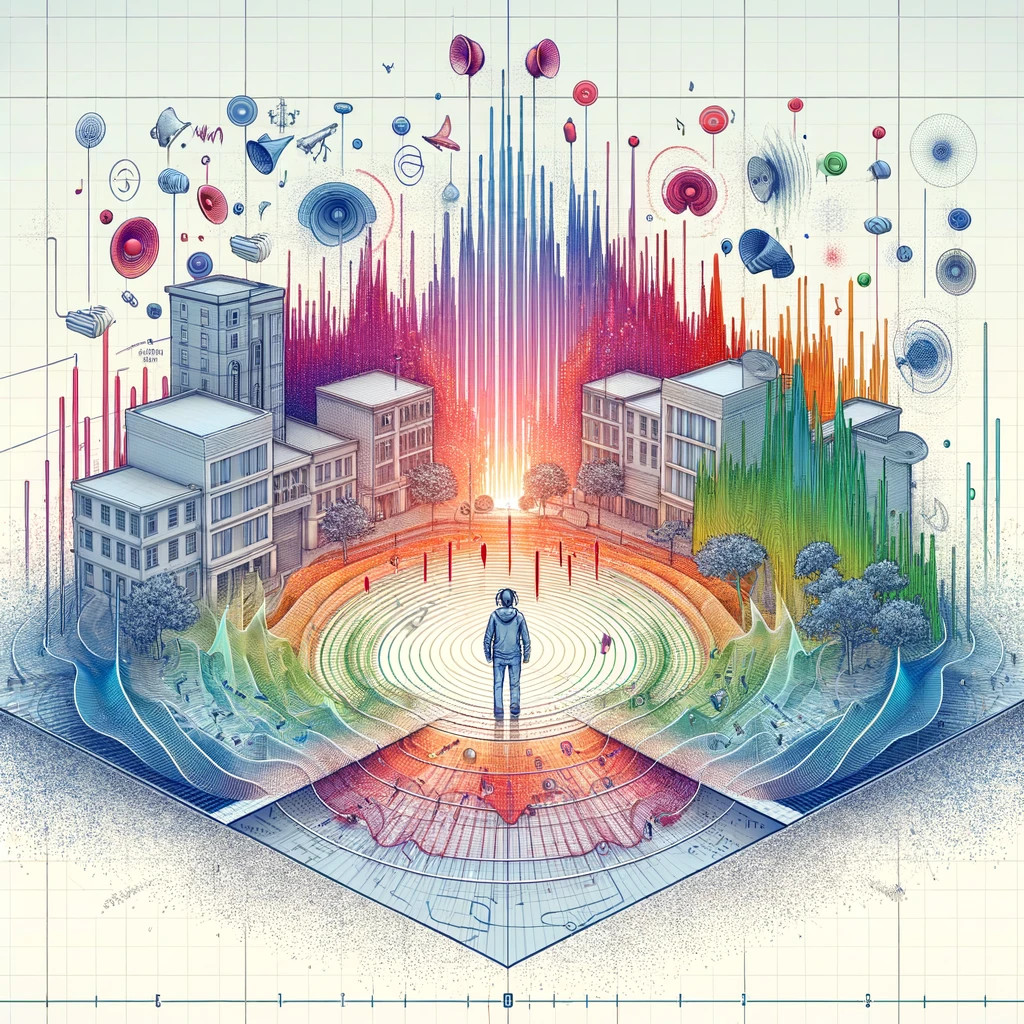
\includegraphics[width=.8\linewidth]{thesis_art}
    \caption[A visualisation of a hypothetical virtual environment where a user is immersed in a rich soundscape perceiving many sound-emitting entities.]{A visualisation of a hypothetical virtual environment where a user is immersed in a rich soundscape perceiving many sound-emitting entities. This visualisation is envisioned and produced by the DALL-E text-to-image model (\url{https://openai.com/dall-e-3})}
\end{figure}

Since the first experiments by~\cite{sutherland1968head} in engineering systems to present users with stimuli to convey three-dimensional virtual objects, research domains around immersive virtual environments have only risen in popularity and become central topics in the major journals and scientific venues in computing.
\acrfull{ve} constantly improve their ability to express virtual worlds in multimodal platforms \citep{rubio2017immersive}. Their applications range from computer games, including serious and educational games, to digital museums, cultural preservation, and architectural design, which have raised the need for realistic and compelling representations of \acrshortpl{ve}. Realism is achieved by emulating the physics of the real world, improving user engagement and performance in tasks in immersive applications. Realism and presence in the audiovisual domains are strongly related to the interaction with scene elements via perception of stimuli \citep{zimmons2003influence, lokki2005navigation}. Sound cues alone, for instance, are sufficient to enable users in \acrshortpl{ve} to pinpoint locations of sound-emitting entities in a scene by using auditory sound localisation, a natural ability associated with the human auditory system.\par
Creating compelling and realistic auditory displays is problematic, providing many challenges in the acoustics and computer graphics research communities due to the complex nature of sound in the real world. As the acoustic principles that govern how sound propagates in space are difficult to reproduce in digital systems, many methods exist, providing variable orders of approximations, depending on the application. Such approaches emulate the wavefield of an environment, simulating how sound interacts with boundaries and scene objects. A subset of these can reproduce phenomena of sound, such as diffraction, reflection, and refraction, which are determinants of realism as they emulate how waves bend around obstacles. Such phenomena make the simulated wavefield dependent on the accuracy of scene geometry and materials represented in a \acrshort{ve} \citep{kuttruff2016room}.\par

Graphics and visual rendering systems are responsible for representing geometry and objects of an environment, defining a relationship between the appearance of materials and the simulated wavefield. This relationship determines realism and presence evoked due to the subjective aspect of auditory and visual perception.
Representation of auditory and visual information varies depending on the human sensory system. The perception of geometry and material in a complex scene is subjective, requiring rendering methods to consider aspects of human perception. 

% intro to audio rendering
Auditory information is paramount to human perception in natural and virtual environments, helping in orientation and navigation, increasing immersion and aiding in task performance \citep{lokki2005navigation, bork2015auditory, shivappa2016efficient}. The sound field perceived by a listener is a function of the shape, dimensions, boundaries and transmission mediums of the surrounding environment. Even though the physics of sound propagation makes realistic audio rendering a challenging task, many proposed approaches allow realistic simulations of sound fields in virtual environments (VEs). Computer games, compelling simulations and digital tourism benefit from realistic audio rendering and improved auditory presence evoked in virtual environments \cite{lokki2002creating, selmanovic2020vr}.

The realism of digital media has increased in recent years thanks to recent advances in computer games technology \cite{rubio2017immersive}. Sound describes entities with respect to the acoustic environment they exist in. As a listener in a sound transmission, the human auditory system is aware of acoustic characteristics manifesting in auditory cues, which enable spatial hearing abilities, such as sound localisation, aiding interaction tasks with objects in the world. Intrinsic acoustic characteristics are dependent on the sound transmission's wavefield, dictated by structural properties of the environment, associated with boundaries and materials, as they interact with sound propagating to the listener's ears. Acoustic rendering methods simulate real or virtual auditory environments by deriving from sound propagation algorithms that discretise the geometrical representation of an environment to synthesise a wavefield. They render spatialised sound adopting signal processing chains to reproduce realistic sound transmission in the simulated wavefield, considering the listener's position, orientation and their physical characteristics, described by Head-Related Transfer Function (HRTF) \cite{hulusic2012acoustic}. \par

% Intro to Audio in XR
AR platforms are suited for a range of use cases within areas of training, digital tourism, or games, thanks to the enhanced interactions with the physical world surrounding the user. An AR platform is a set of technologies interfacing with the user via audio-visual and holographic displays, gesture, eye, and body tracking, and with the physical world via computer vision, scene understanding, space reconstruction, and spatial mapping techniques. This broad range of sensing technologies opens avenues for addressing tasks within research domains where users interact with entities in AR space. Accessibility, for instance, is a research domain benefitting from the development of this platform by helping users with disabilities navigate and understand their surrounding scene, leveraging the sensing data provided by the platform and performing speech recognition or scene understanding techniques \citep{mehra2020potential}.


The increasing popularity of immersive media proliferating within an increasing number of industry and research domains \citep{park2022metaverse}, enabling HMDs to support applications ranging from training scenarios, education, social learning, operation learning \citep{harris2020effect, ahir2020application} to entertainment or gaming \citep{yuen2011augmented, ke2018virtual} or to digital tourism and cultural preservation use cases \citep{schofield2018viking, selmanovic2020cultural}. AR applications in modern HMDs, e.g. the Microsoft Hololens 2\footnote{\url{https://www.microsoft.com/en-gb/hololens}\label{note:ms-hl2}}, can provide real-time space reconstruction, spatial mapping, and scene understanding features\footnote{\url{https://learn.microsoft.com/en-us/hololens/hololens2-hardware}\label{note:ms-hl2-hw}}. Such features have unlocked crucial potential in the sound rendering subdomain, as emerging novel pipelines allow acoustic simulation techniques to be deployed to AR HMDs, as discussed in Chapter~\ref{ch:ar-pipeline}. As a result, users experiencing holographic content projected onto their surroundings can perceive realistic sound propagation from holograms. Experiencing realistic sound rendering in AR directly impacts the above-mentioned industry domains and research as HMDs become more ubiquitous and accessible. \par
These example applications and use cases of AR with modern HMDs rely on auditory stimuli for conducting activities or completing tasks in VEs, such as navigation, locomotion, or entity localisation. As discussed in Chapter~\ref{ch:Background}, the hearing sense relies on acoustic information encoded in auditory stimuli to predict or triangulate the position of sound-emitting objects within the hearing range.


\section{Significance}
A novel aspect of the proposed work is the application of computer vision methods to infer acoustic data associated with materials and boundaries in environments to enable sound rendering systems such as acoustic simulation methods, to adapt to unseen complex scenes in materials.
Potential contributions of this novelty include Augmented Reality (AR) applications \citep{liu2018technical}, where users can control interactions between virtual objects and the real world. A possible outcome from the proposed work would allow AR applications to render sounds emitted from virtual objects considering acoustic aspects of real environments. \par
The system would apply to computer games technology, contributing to computer games, serious games, architectural acoustics and digital tourism. 
Architectural acoustic applications would benefit from automated reconstructions of auditory spaces from real environments, allowing designers to create and test acoustic models with AR applications or game engines \citep{berardi2016acoustic}. Digital tourism, besides, would benefit from improvements in sound rendering pipelines to let users experience and interact with reconstructions of places of cultural interest \citep{schofield2018viking}. \par
The need for realistic audio in computer games is of growing importance as it allows players to immerse in virtual worlds. Spatialising sound in three-dimensional worlds, reflecting acoustic features of space, improves the performance of tasks associated with auditory cues, enhancing the overall experience and quality in games. 
Activities in VEs using auditory cues, such as navigation in space and sound localisation are fundamental in simulations and training applications \citep{lokki2005navigation}. Hence, sound rendering systems are of crucial importance in these fields.

\section{Research Aim}
\begin{figure}[htbp]
    \centering
    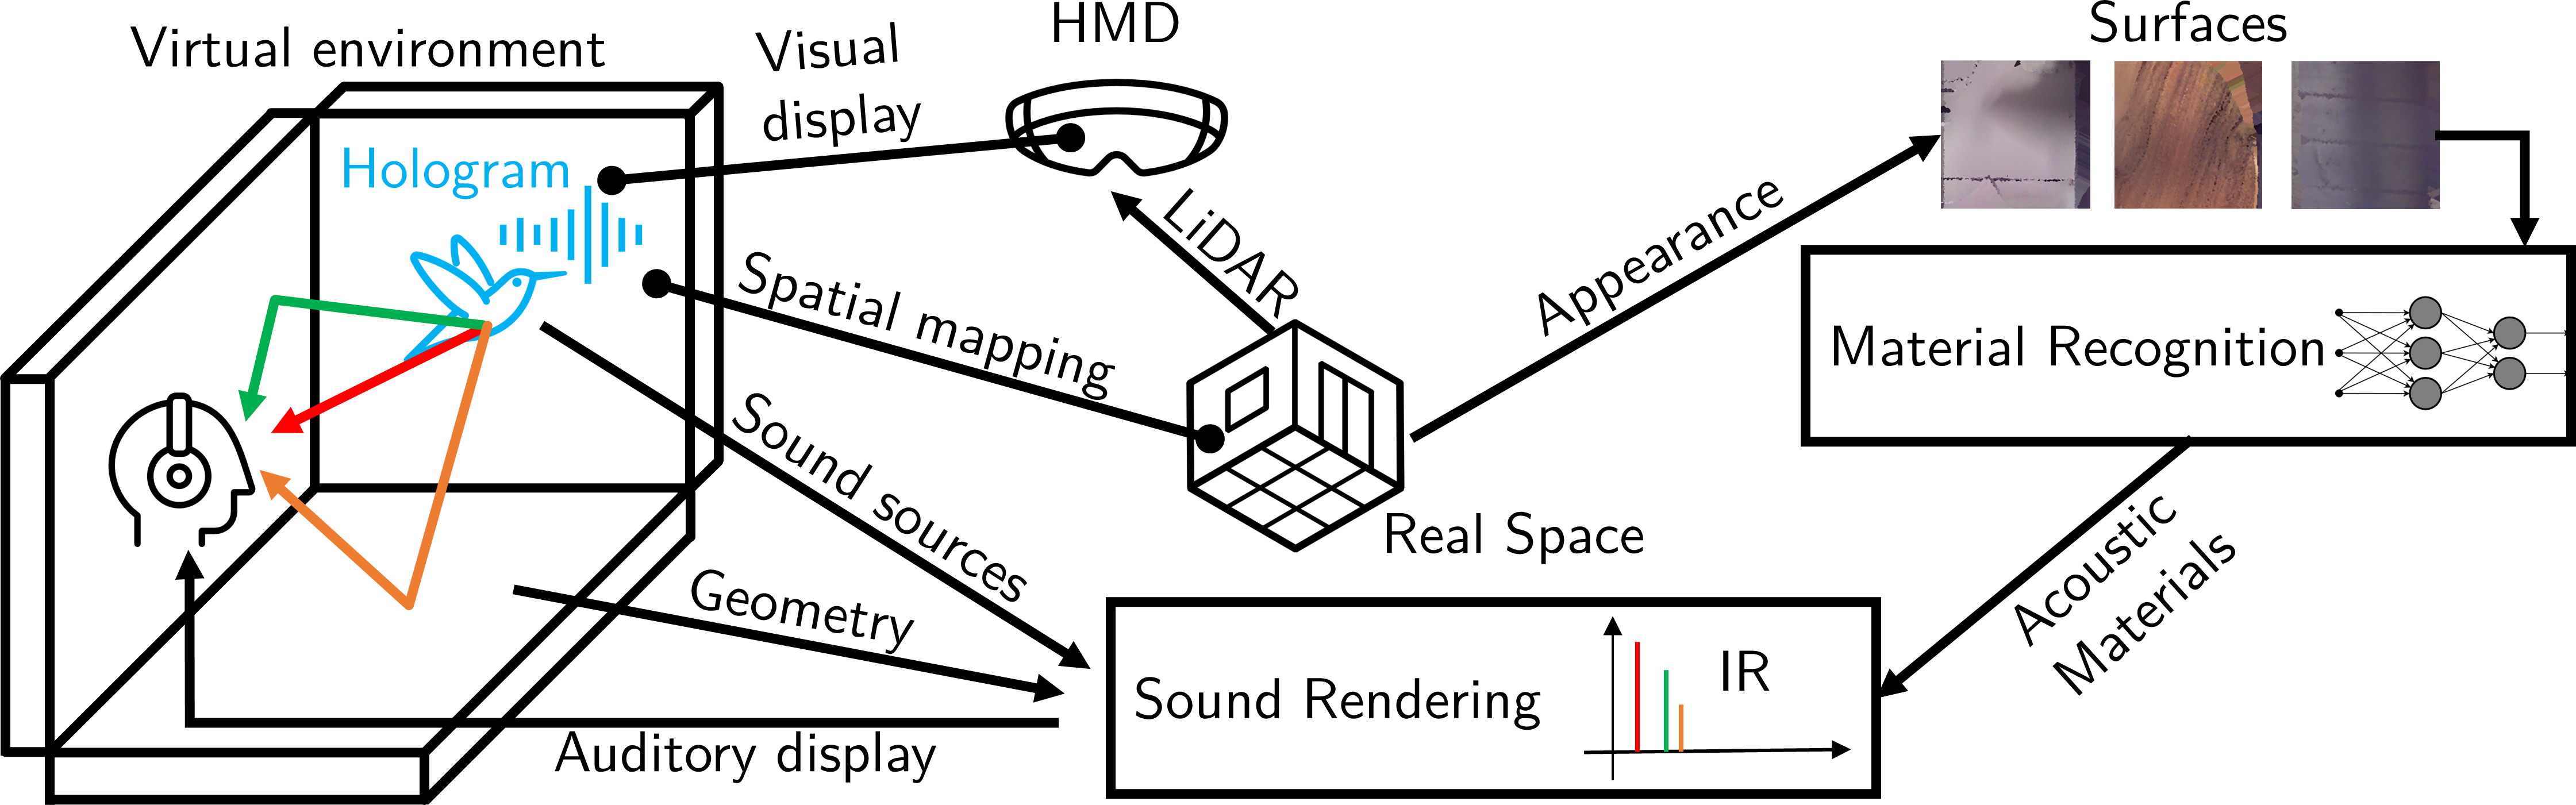
\includegraphics[width=1\linewidth]{phd_functional_diagram}
    \caption{Overview of the interactive acoustic rendering system for AR proposed as part of the thesis work.}
    \label{fig:proposed-system-diagram}
\end{figure}
The proposed work aims to explore rendering pipelines with respect to sound propagation in VEs, studying the relationship between the perceived wavefield and the environment’s visual representation: materials, structural geometry and physicals characteristics of objects in complex scenes.


\section{Objectives}\label{sec:thesis-objectives}
\begin{itemize}
    \item To review the current state of audio rendering in virtual environments, assessing their limitations, realism and computational requirements to  investigate their applications in real-time acoustic simulations for complex scenes.
    \item To explore how, in modern approaches to acoustic simulations, visual representations of materials relate to simulated soundfields.
    \item To design and test systems to automatically attribute acoustic materials to scene geometry in virtual environments, recognising and distinguishing between materials in the acoustic and visual domains.
    \item To study and evaluate the application of sound rendering methods with acoustic material recognition.
    \item To design and propose a novel pipeline for acoustic rendering applied to augmented reality platforms.
    \item To investigate psychoacoustic and human factors in auditory displays created by the proposed pipeline by testing an augmented reality prototype.
\end{itemize}

\section{Thesis Structure}

\begin{figure}[htbp]
    \centering
    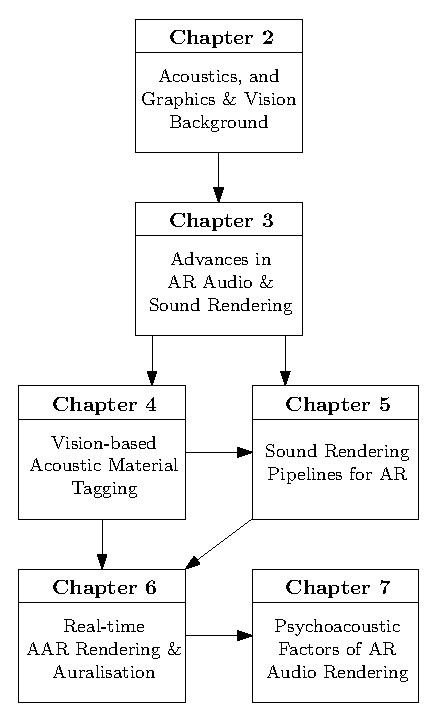
\includegraphics[width=0.6\linewidth]{thesis-structure}
    \caption{Structure and dependency graph of Chapters of this thesis. Introductory and conclusive Chapters, \ref{ch:introduction} and \ref{ch:Conclusion} respectively, omitted for simplicity.}
    \label{fig:thesis-structure}
\end{figure}

\section{Chapter List}
\textbf{Chapter~\ref{ch:introduction}} ``Introduction'' presents the goal and objectives to the reader, starting from the rationale and factors motivating this research, providing background on research domains of interest, and illustrating the contributions and how these are structured throughout the Chapters.

\textbf{Chapter~\ref{ch:Background}} ``Background Research'' provides the reader with foundations on wave physics, sound propagation, acoustic data in digital systems, as well as computer graphics in the context of handling and representing virtual environments. The reader is also introduced to elements of machine learning to provide grounding for vision-based scene understanding systems designed as part of the thesis aim.

\textbf{Chapter~\ref{ch:litReview}} ``Advances in Visual-Acoustic Mapping and Sound Rendering Pipelines'' reports relevant bodies of literature relevant to research and industry domains overlapped by the proposed overarching system. Limitations of the current state of industry and research on these domains are reviewed alongside visions and research directions identified by authors, defining the contributions discussed across the thesis.

\textbf{Chapter~\ref{ch:Materials}} ``Methods for Acoustic Characteristics Retrieval from Complex Virtual Environments'' introduces the design and application of computer vision methods for extracting acoustic characteristics from virtual environments, which constitute building blocks for the proposed pipeline and address acoustic material tagging, a crucial problem in the domain of sound propagation for virtual environments.

\textbf{Chapter~\ref{ch:acousticrendering}} ``Geometrical Acoustics Rendering Pipelines for Augmented Acoustics'' integrates acoustic material tagging systems with standard acoustic rendering techniques based on approximating acoustic waves with geometrical primitives. This Chapter aims to provide a baseline acoustic renderer for designing the interactive AR pipeline proposed in the following Chapter.

\textbf{Chapter~\ref{ch:ar-pipeline}} ``Towards Scene-Aware Acoustic Rendering Pipelines for Augmented Audio Reality'' demonstrates the design of the proposed pipeline, expressed by the overarching research aim, as an end-to-end system for Augmented Reality Head-Mounted Displays, illustrating technical components and workflows for achieving real-time interactions. Considering related work reviewed by Chapter\ref{ch:litReview}, visions, impact, and future research are discussed, indicating avenues for expansions.

\textbf{Chapter~\ref{ch:ar-pipeline}} ``Psychoacoustic Characterisation of Rendering Pipelines for Augmented Acoustics'' deploys a prototype to an augmented reality platform in order to conduct a set of psychoacoustic tests on the pipeline illustrated by the previous Chapter. Here, a novel methodology and framework for testing the characterisation of sound rendering pipelines are evaluated and discussed.

\textbf{Chapter~\ref{ch:Conclusion}} ``Conclusions'' provides a high-level discussion on the results gathered from objective and subjective experiments gathered by testing components of the proposed system, reflecting on broader impact, detailing potential use cases, and recommending future expansion avenues.

\section{Contributions}
The main contributions of this thesis are the proposal, design, prototyping, and testing of a novel pipeline for generating realistic auditory displays in augmented reality platforms, leveraging the potential that modern hardware for holographic rendering has unveiled over the last decades. These contributions represent a stepping stone towards realistic and physically-based auditory interactions in immersive applications, allowing users to understand, reason, and act within a virtual environment from acoustic information conveyed by the augmented reality platform.
These contributions stem from components of the pipeline developed and tested, addressing research questions associated with the design of an end-to-end system. Chapters~\ref{ch:Materials},~\ref{ch:acousticrendering}, and~\ref{ch:Evaluation} present novel systems to address such research questions adopting bespoke methodologies and evaluations. The following list briefly summarises the contributions of this work:
\begin{itemize}
    \item a novel pipeline for realistic acoustic displays for augmented reality platforms;
    \item two novel systems for retrieving acoustic characteristics from virtual environments;
    \item novel testing methodologies for evaluating system for acoustic characteristics retrieval, comparing simulated against real soundfields;
    \item two sound rendering systems integrating methods for acoustic characteristics retrieval;
    \item a study evaluating the proposed sound rendering methods;
    \item a perceptual evaluation investigating psychoacoustic factors of a prototype of the proposed system.
\end{itemize}

% \fullcite{colombo2021texture}
% \chapter{Background}\label{ch:Background}

The following Sections introduce a body of knowledge from domains intersecting the overarching aim of this work, providing the reader with the necessary tools to dissect the components presented throughout the thesis. This Chapter begins by introducing basic sound physics, wave theory, and human perception as they define basic concepts of auditory interactions in the physical and virtual worlds.\par
Since a human listener is a link in the chain of the system proposed as part of this work, this Chapter will introduce basic psychoacoustic concepts linking the objective and technical aspects of sound rendering systems to human factors and subjective perception.

\section{Background on Human Hearing}
\subsection{Characteristics of the Human Hearing System}
The \acrfull{has} generally comprises two ears on either side of the human head, and each ear is a system that can be divided into three main parts: the outer ear, commonly referred to as the ear; the middle ear; and the inner ear. The outer ear, also referred to as the pinna, is shaped like a shell, is made of cartilage and skin, and serves both as protection for the system of receptors, ossicles, and nerves within the middle and the inner ear and a funnel that collects sound energy and transmits it to the middle ear via the outer ear canal. The outer ear canals are largely responsible for the frequency response of the \acrshort{has}. 
Auditory stimuli are sent to the brain via sensory cells that are surrounded by fluids displacing according to the received sound pressure. The middle ear converts sound pressure from the ear canal to displacement to these fluids, which send signals to the brain. This part of the ear is able to withstand variations of air pressure arriving at the outer ear and is responsible for matching different impedance magnitudes between the air or the medium in which sound is arriving at the apparatus and the impedance of the fluids in the inner ear.
The inner ear comprehends the vestibular system, a sensory system that allows humans to sense their spatial position, perceive rotation or displacement, and achieve balance and the cochlea. The cochlea, shaped like a snail, is embedded in the hard temporal bone, part of the skull \citep{zwicker2013psychoacoustics}.
\begin{figure}
    \centering
    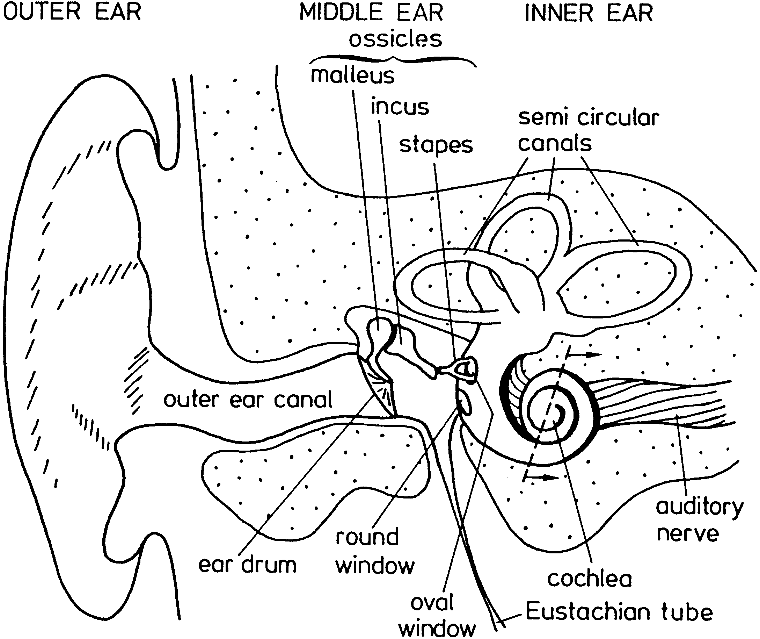
\includegraphics[width=1\linewidth]{human_ear}
    \caption[Overview of the human hearing system]{Overview of the human hearing system \citep{zwicker2013psychoacoustics}}
    \label{fig:human_hearing_system}
\end{figure}

\subsection{Introduction to Psychoacoustics}\label{sec:bg-psychoacoustics}
The \acrshort{has} enables one of the fundamental functions of perception of surrounding space. In humans and species of the animal kingdom, hearing is the basis of many mechanisms, such as communication or survival instincts. Such mechanisms are neural processing applied to auditory stimuli arriving at the hearing system in order to compute tasks or solve problems, such as communicating using acoustical data or pinpointing the location of a sound-emitting entity relying on auditory stimuli. These are example applications or problems that can be solved by processing acoustical data interpreted by the \acrshort{has}.
Psychoacoustics investigates how the \acrshort{has} responds to auditory stimuli and investigates applications like loudness perception, localisation, lateralisation, or room volume estimation. The understanding of psychophysical responses of the \acrshort{has} to acoustical data in environments influences everyday activities that involve communicating, listening to musical instruments, or delivering messages to an audience of multiple listeners. The design process of built environments, infrastructure, or concert halls takes into account psychoacoustic factors to facilitate or improve human perception in specific environments during specific activities.

\subsection{Sound Localisation}
\begin{figure}
    \centering
    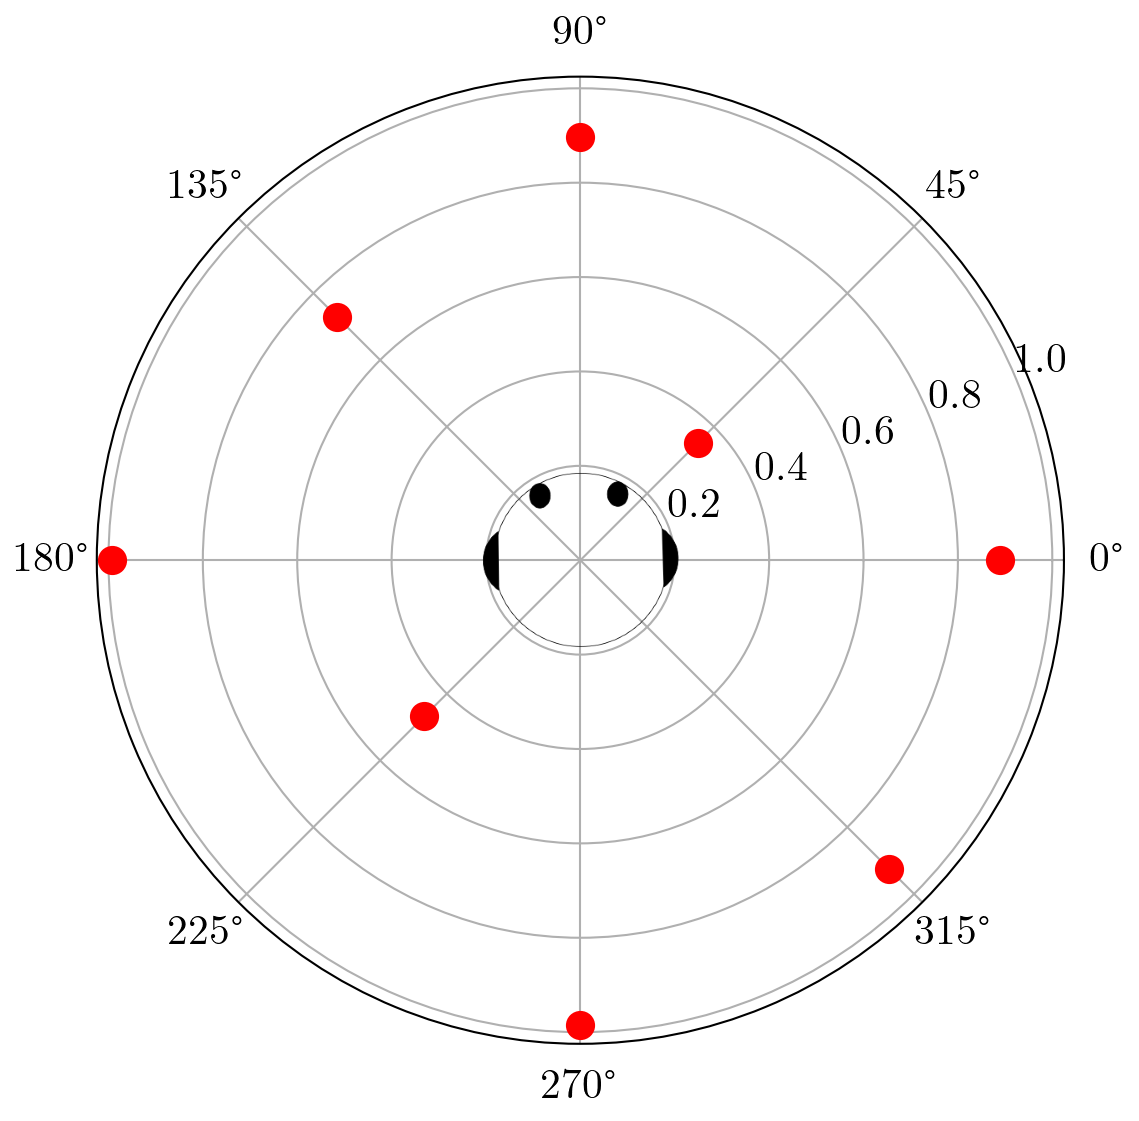
\includegraphics[width=1\linewidth]{localisation_example}
    \caption[Sound localisation visualised]{Sound localisation is the ability of the \acrshort{has} to pinpoint the position and direction of sound sources, red dots, at different directions and distances around the listener, centre.}
    \label{fig:localisation-listener}
\end{figure}

\subsection{Masking}
types of Masking

\subsection{Just-Noticeable Differences}

\section{Acoustic Theory}
\subsection{Sound Propagation in Real and Virtual Environments}
Sound propagation is a transmission of energy in a sound field, which can be thought of as a superposition of sound waves travelling in a medium. In this work, we consider air as the sound propagation medium, which is assumed to be homogeneous, i.e., determining a constant velocity of sound $c$ expressed as: 
\begin{equation}
c = (331.4 + 0.6\Theta)~\frac{m}{s}   
\end{equation}
where $\Theta$ is the temperature in centigrade.
A vibrating object in a sound field causes air particles to move, initiating the transmission of energy in the field. Such an object is defined as a sound source, and if the intensity and frequency of the vibrations are within the perceptible range of the human hearing system, a listener may experience sound emitted by the said sound source.
In everyday sound transmissions, the air within sound fields is not at rest and features many inhomogeneities caused by external factors affecting the state of its particles, such as windows or air conditioning systems. However, according to \citep{kuttruff2016room}, such inhomogeneities are imperceptible, and generally, the air temperature has a perceptual effect on sound transmissions, especially in large concert halls and open spaces. Air temperature effects can be neglected in indoor sound propagation.

\subsection{Sound Transmissions}
Energy in the sound field, transferring from a vibrating sound source to the hearing system of a listener, is perceived as an acoustic signal characterised by varying intensity and frequency. 
The intensity of 
Sound pressure, amplitude, sampling 

\subsection{Acoustics in Real Environments}
\begin{itemize}
    \item Definition of a sound field
    \item Characterisation of sound fields
    \item Objective metrics describing sound fields; Farina's descriptors.
    
\end{itemize}


\section{Digital Representation of Audiovisual Information}
\label{sec:DSP-background}
The following section will introduce background knowledge on Digital Signal Processing relevant to the representation of acoustic signals in digital systems and the manipulation of auditory stimuli in virtual environments. Digital Signal Processing methods and techniques provide building blocks for the construction of realistic 3D auditory displays in immersive technology.

\subsection{Digital Signal Processing for Acoustic Rendering}
Digital Signal Processing (DSP) is the science of analysing time-dependent physical processes. The acoustics realm deals with analogue signals and digital signals, terms used to indicate a continuous variation of amplitude values in a physical process. Electricity utilised to drive loudspeakers is an example of an analogue signal, expressing continuous changes in voltage applied to magnets to displace the position of a cone. The cone displacement causes pressure differences in air particles, transforming such changes in voltage to changes in air pressure, which the human auditory system interprets as sound. Acoustic signals consist of one or multiple sound waves oscillating, where each wave is an oscillation of energy at regular intervals; the duration of each interval determines the wavelength $\lambda$, and oscillations are measured as frequency in Hertz (Hz). \par
On the other hand, a digital signal is a discrete representation of a continuous physical process, resulting in a sequence of measurement samples of an analogue signal expressed as amplitude values over time. Figure 1 shows the difference between a continuous signal and a discrete signal: digital signal is represented with stems to indicate its nature of quantised measurements over time, abscissa, as opposed to a continuous change in amplitude, ordinate. The discrete nature of a digital signal has inherent problems and advantages that relate to the time interval between measurements: a digital signal representing an analogue one will always be an approximation of the continuous process as the system may change its state between measurement intervals. The approximated nature of digital signals causes information loss, which is counteracted by theories shown later, but allows digital systems to store and process acoustical data efficiently.\par
DSP applies to both, but in this book chapter, we will only focus on the branch of DSP that deals with digital signals. Digital systems like computers are used to process stored acoustical signals for several reasons, such as storing recordings of anechoic acoustic signals that simulation software can then process to generate realistic acoustic simulations, expressed as a processed digital signal. \par
\begin{figure}
    \centering
    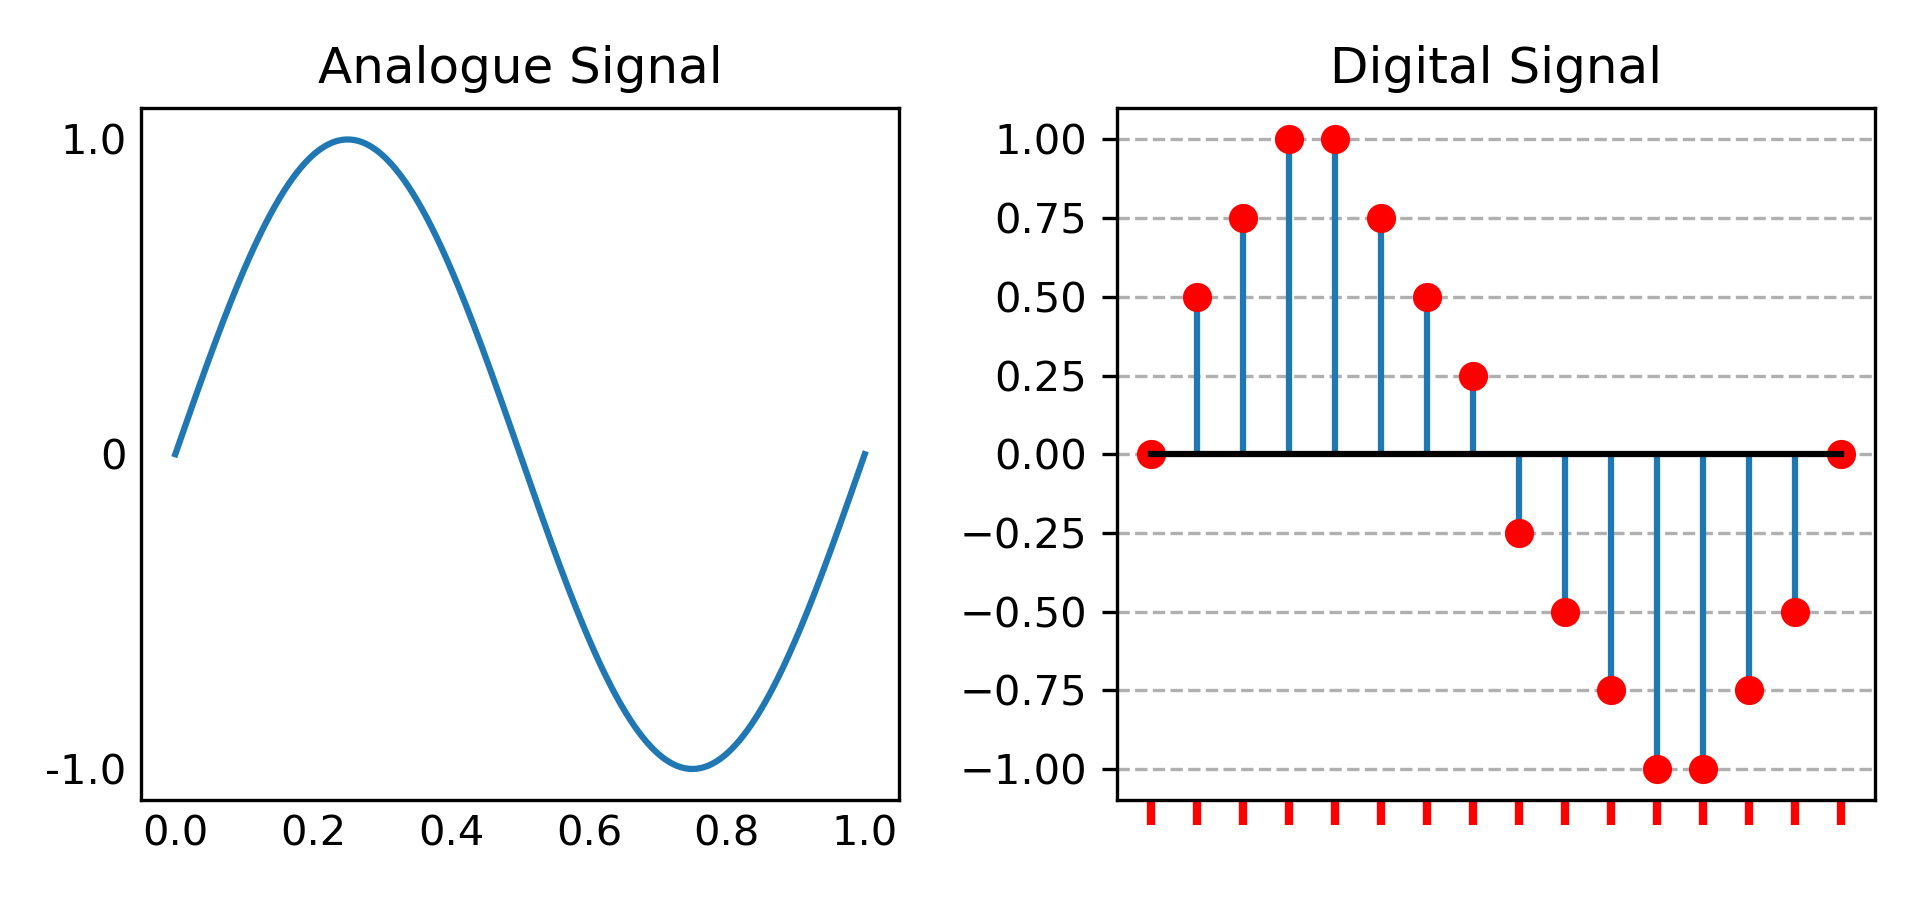
\includegraphics[width=1\linewidth]{analogue_digital}
    \caption{Analogue and digital signal: the left axes show a continuous signal, and the right axes show a discrete sampled representation.}
    \label{fig:analogue-digital-signal}
\end{figure}

The process of converting continuous signals to digital information involves taking measurements of the amplitude of a continuous signal at regular time intervals. There are two dimensions in which the analogue signal is measured during this process, the amplitude and time, respectively, the abscissa and the ordinate of Figure~\ref{fig:analogue-digital-signal}.\par
Due to the physical limitations of digital technology, A/D converters can only take a finite number of measurements between time intervals, and they have limited accuracy in representing amplitude levels. In Figure \ref{fig:analogue-digital-signal}-b, it is possible to see how an A/D converter sees analogue signals: given an acoustic continuous signal as input, it takes amplitude samples at every time step, marked with by red ticks, and measures using the available amplitude levels (the dotted horizontal lines). As a result, the process outputs a series of data points, the red dots, approximating the input, and the resolution and fidelity of the approximation depend on the time elapsed between time steps and the available amplitude level points. There are standards to ensure the reproduction and manipulation of acoustical signals in digital systems with an appropriate fidelity, such as the ``Red Book'' IEC 60908 standard, adopted for the Compact Disc music format, determining that digital signals must be represented by 44.100 measurement samples per second, at 16bit amplitude resolution. 16-bit refers to the binary representation adopted by digital systems to store amplitude values, allowing $2\textsuperscript{16}=65,535$ possible amplitude levels. The sampling frequency, the number of measurements per second, is calculated in Hertz (Hz), and it is a fundamental property of digital signals that must be taken into account for almost all types of audio manipulation and analysis involved in acoustical applications and it paramount to correct reconstructions of any acoustic information in any digital system. \par
The Nyquist-Shannon sampling theorem is used to ensure a digital system reconstructs an analogue signal correctly. The theorem proves that a wave must be sampled at least twice during each oscillation period. A periodic wave oscillating at $20kHz$, which is around the maximum perceivable frequency in the human hearing range, would need to be sampled at least $40,000$ per second; hence, the standard $44.1kHz$ sampling rate. In Figure~\ref{fig:aliasing}, for instance, a $50Hz$ signal is sampled at $90Hz$, below the $100Hz$ Nyquist sampling frequency, causing aliasing, an incorrectly reconstructed signal that will be able to oscillate at a maximum frequency of $45Hz$.\par

\begin{figure}
    \centering
    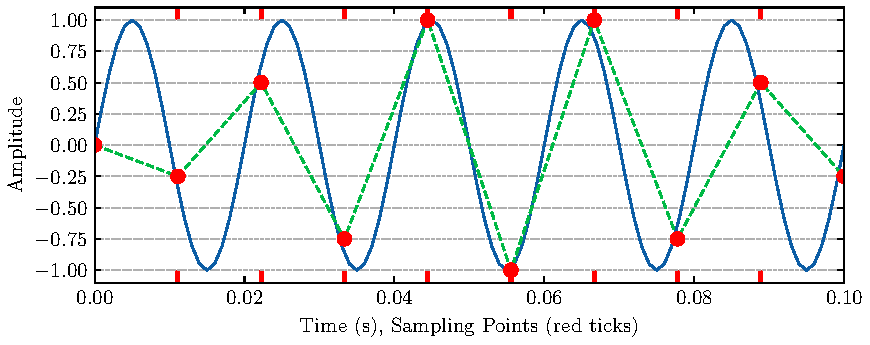
\includegraphics[width=1\linewidth]{aliasing}
    \caption{The blue signal is being sampled at a sampling frequency lower than the Nyquist frequency, causing aliasing, an incorrect reconstruction of the digital signal, as opposed to Figure~\ref{fig:analogue-digital-signal} that shows a correctly reconstructed signal. As a result, the dotted green signal is created instead, having a frequency between $0Hz$ and the sampling frequency.}
\label{fig:aliasing}
\end{figure}

\subsubsection{Analysis of Digital Signals}
Acoustical signals are often analysed in the time domain, as varying sound pressure levels over time, or in the frequency domain. By considering acoustical signals as a Fourier series, a function composed of sine or cosine primitives, the frequency domain representation determines how the power of an acoustical signal is distributed in a range of sine and cosine functions with wavelengths usually ranging from the minimum to the maximum perceivable frequencies of the human auditory system - low to high frequencies. Time- and frequency-domain representations are often used for both analysis and manipulation of acoustical signals, often adopted in tasks like determining the effects of an environment in the perception of sound emitted by an object and arriving to a listener in said environment \cite{ballou2013handbook}. \par 
In acoustics for interactive applications, engineers often adopt the Discrete-Time Fourier Transform (DTFT), a Fourier series for digital signals, which is one of the fundamental concepts in DSP. It takes a sequence, such as the signal represented in Figure\ref{fig:analogue-digital-signal}-b and generates $N$ complex numbers, representing power across $N$ sinusoids. The DTFT, as defined by classic DSP theory \cite{shenoi2005introduction}, transforms a signal $x_n$ containing samples $x_0, x_1,~\dots, x_{N-1}$ into a series $X_k$ of complex numbers $X_0, X_1,~\dots, X_{N-1}$. $X_k$ is defined by:
\begin{equation}
    X_k = \sum_{n=0}^{N-1} x_n~\cdot~e^{-\frac{i2\pi}{N}kn}
\end{equation}

\begin{figure}[htb]
    \centering
    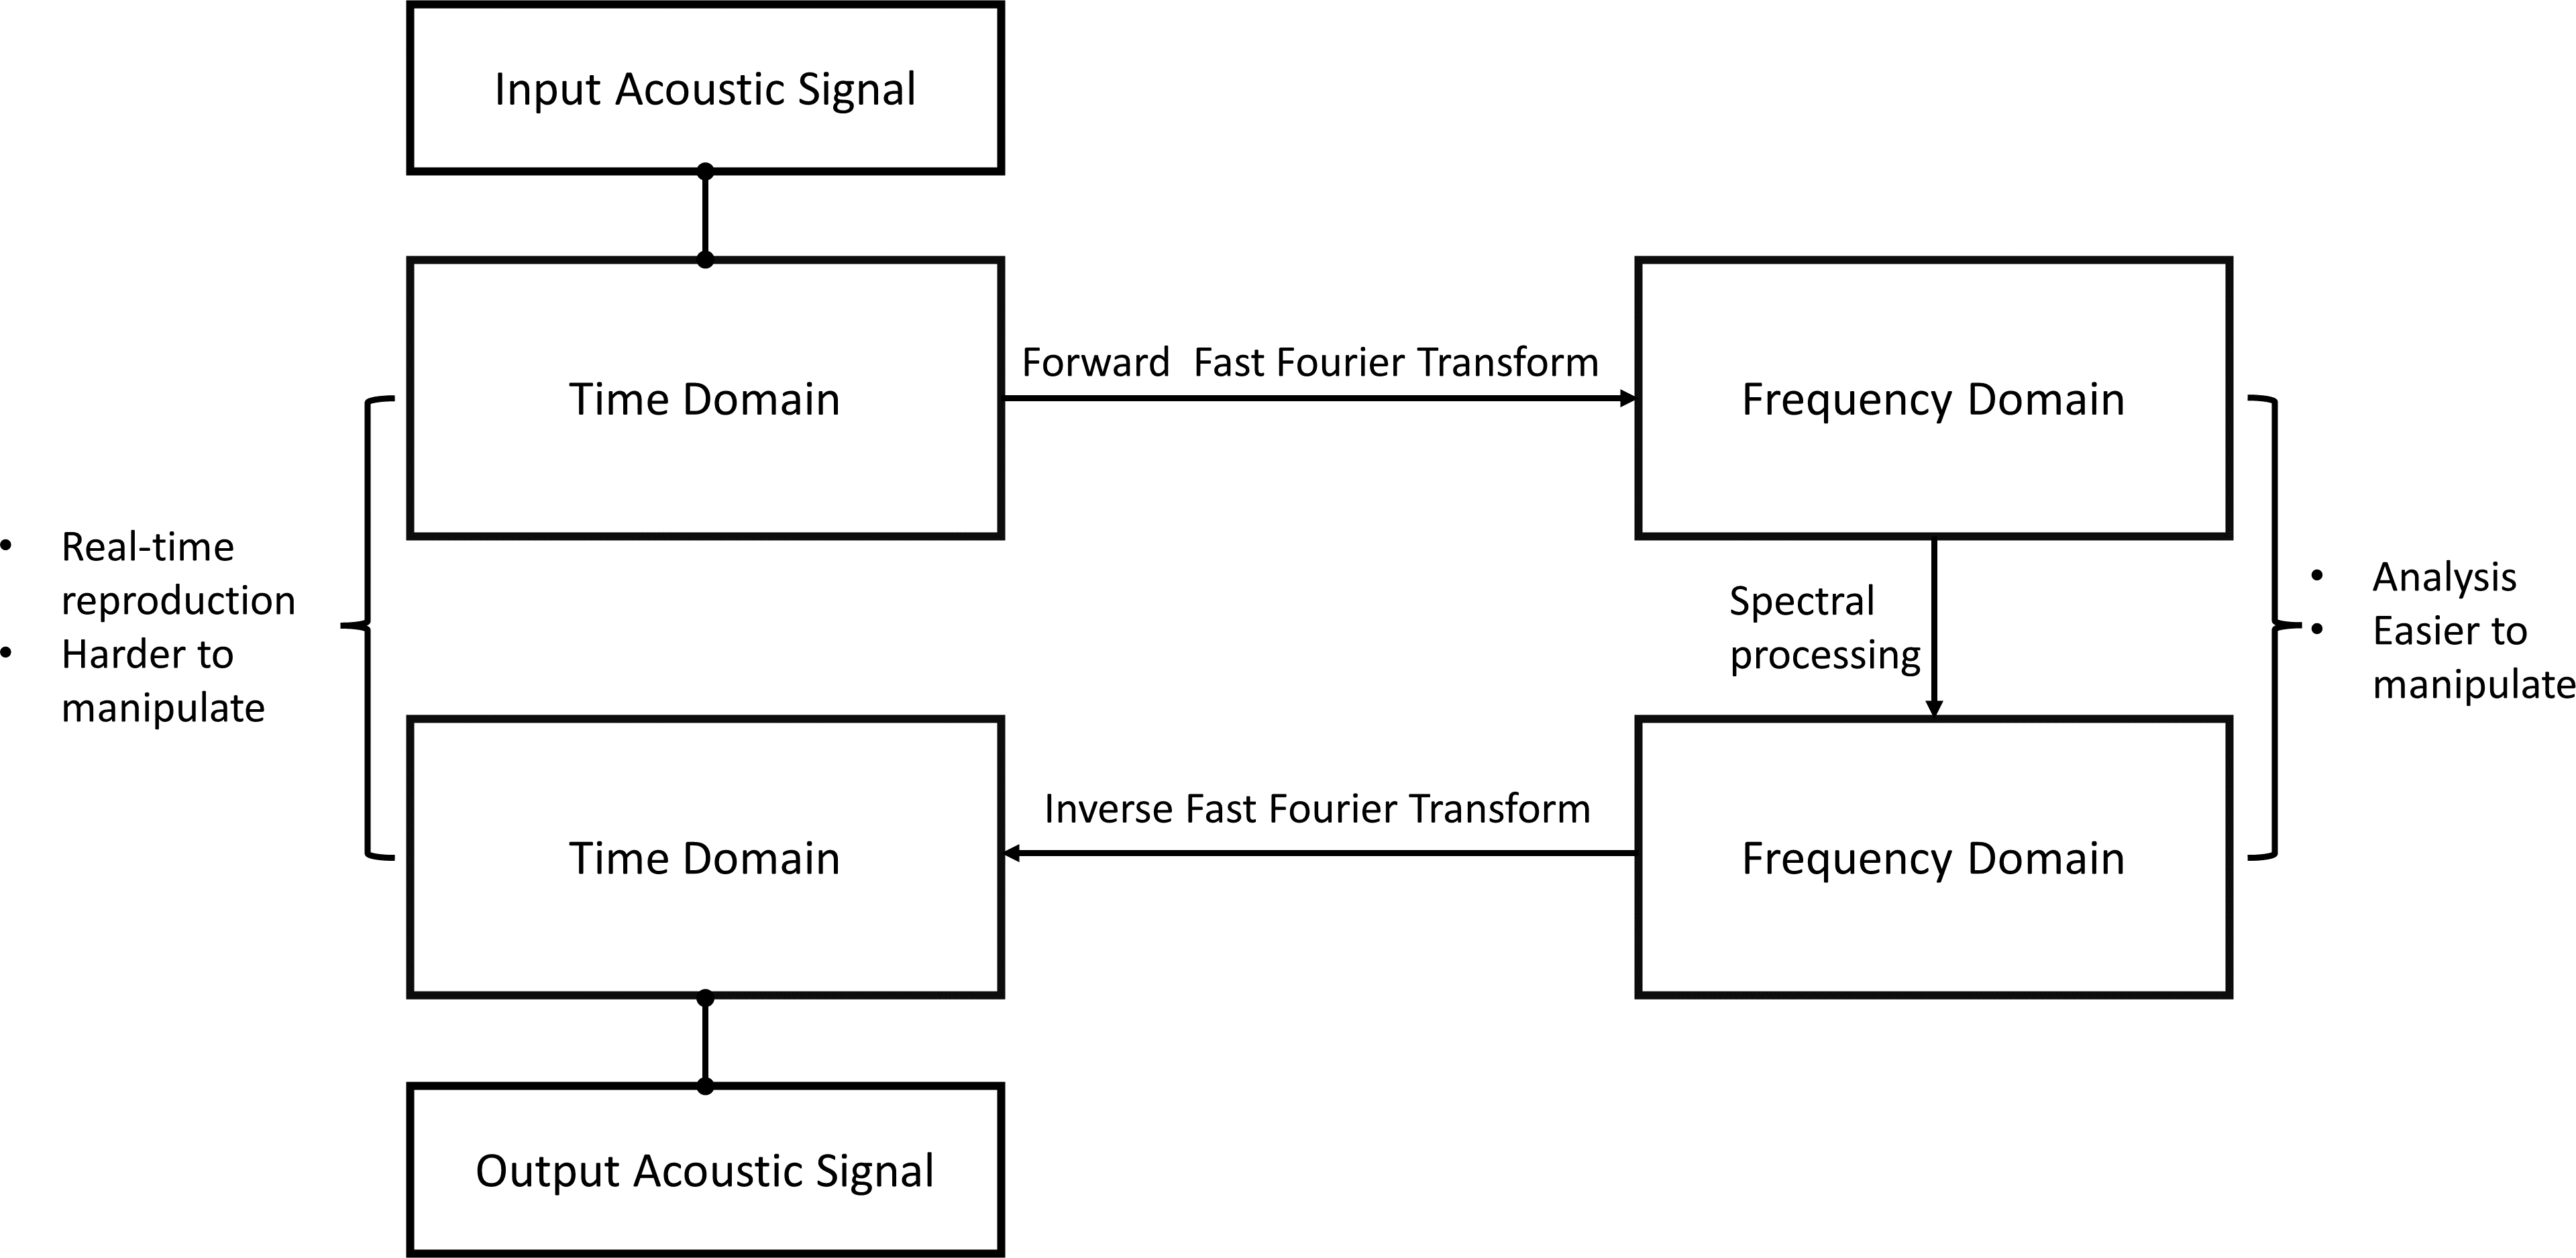
\includegraphics[width=1\textwidth]{DFT}
    \caption{A basic chain for signal processing aimed at analysing or manipulating signal in auralisation, visualisation, or interactive applications. Analysis and processing of digital signals in the time domain is generally a hard task due to the complex nature of the function representing audio. The frequency-domain representation eases analysis and manipulation problems even with the added computational load of transforming between the two domains.}
    \label{fig:DFT}
\end{figure}

\subsection{Image Processing Fundamentals}\label{sec:image-processing}
\begin{itemize}
    \item digital images
    \item basic imge processing techniques
    \item filters
\end{itemize}

\subsubsection{Binaural Room Impulse Responses}\label{sec:ir-definition}
Common approaches to acoustic simulations involve the approximation of acoustic phenomena affecting a sound transmission occurring within a given environment between a sound source and a listener. To represent the result of such a simulation as a measurable process, where the environment is thought of as a dynamic system, Impulse Responses (IR) are used. IRs describe the effect that a system has on a sound transmission as a function of time. From DSP theory, there are several variations of IRs that the fields of immersive acoustics borrow to model several dynamic systems that affect how the human auditory system perceives soundscapes. Figure~\ref{fig:audio_rendering_chain} shows how the auditory display is affected by interconnected systems associated with aspects of the soundscape. Time invariance is the fundamental property of these systems, making it possible to model their effect as an IR by observing their response to a Dirac-Delta function, which is a function whose value is zero except at the origin, where it is infinite. In practical terms, the Diract-Delta function is an infinitely narrow energy spike often used to excite the system and obtain a response across the frequency spectrum over time. In DSP terms, the function is simply represented as a finite sequence of numbers, the Finite Impulse Response (FIR), representing amplitude levels of the output of the system over time, given an input, commonly used to measure the effects of time-invariant linear systems like amplifiers or loudspeakers.\par
In the acoustic domain, the FIR adapts to several tasks, like modelling the acoustic fingerprint of a space with respect to a source and listener by observing, at the listener, a Dirac-Delta-like signal being emitted by the source. Such IR is differentiated from standard IRs and referred to as a Room Impulse Response (RIR); such distinction has emerged from the ongoing research in techniques and methods for measuring responses from real spaces, also due to the chaotic nature of room acoustics and real soundfields \citep{farina07}. 
IRs, as well as measuring the acoustic fingerprint of spaces, can extend as far as measuring the effect of the human auditory system on the perception of the soundscape, and there are methods for modelling how anthropometric characteristics of the human body affect sounds arriving at both ears. Such IRs are defined as Binaural Room Impulse Responses: they extend RIRs by providing individual responses for both ears. BRIRs are a representation of Head-Related Transfer Functions (HRTFs), a function that describes how the anatomic features, rotation, and position with respect to a sound source affect the arrival of sound to the ears. Figure~\ref{fig:rir-spectrum} is an example of a monaural RIR, shown both in the time and frequency domain. 
\begin{figure}
    \centering
    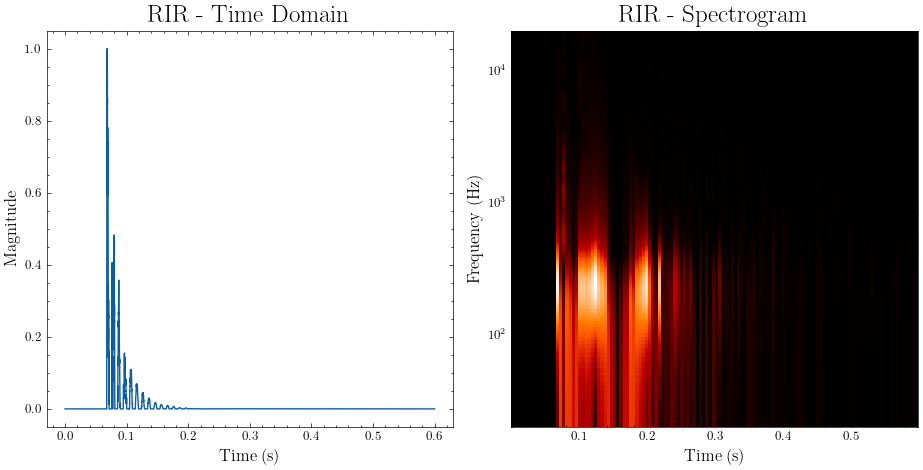
\includegraphics[width=1\linewidth]{rir_spectrum}
    \caption{Both time and frequency-domain, left and right respectively, representations of a Room Impulse Response (RIR). The time domain representation shows the magnitude of sound paths from a sound source to a receiver over time. The frequency domain representation shows how the energy of sound paths is distributed across the frequency spectrum over time, which is visualised with an infrared colour map.}
    \label{fig:rir-spectrum}
\end{figure}

\section{Common Approaches to Immersive Acoustics}
Achieving a convincing immersive acoustic experience is no trivial task, and various techniques and methodologies have been developed to address this complex challenge. These approaches must consider sound's spatial, temporal, and perceptual aspects and the HAS's intricate response to auditory stimuli.

\subsection{3D Sound Reproduction Techniques}
Sound reproduction for immersive acoustics can be defined as a rendering problem concerning providing a listener with synthetic believable auditory stimuli perceived as belonging to a specific space. The rendering is often engineered by adopting a system that has complex scenes and scene elements as input and an acoustic signal as output. 
\begin{figure}
    \centering
    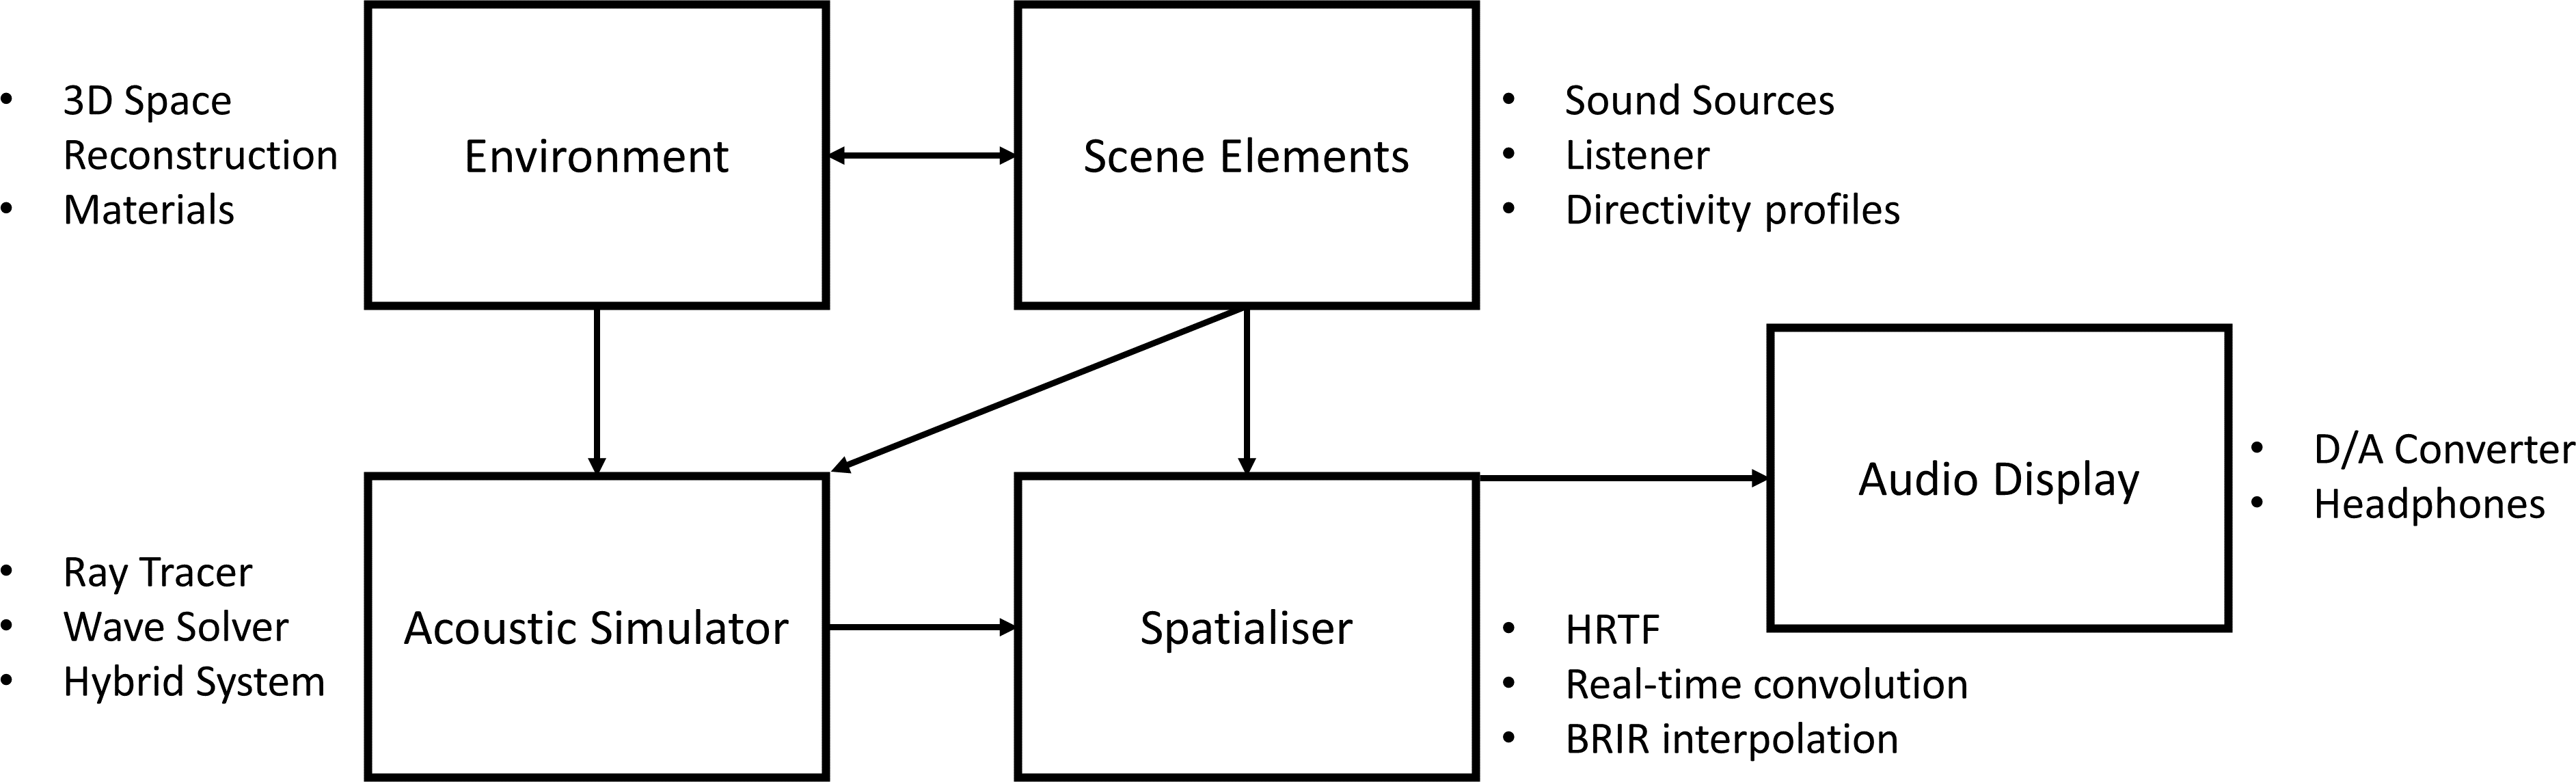
\includegraphics[width=1\textwidth]{spatialiser_system_overview}
    \caption{An example chain of 3D reproduction based on acoustic simulators: an environment is fed into acoustic simulators to produce BRIRs. A spatialiser system consumes these to generate an audio signal considering the listener and scene elements.}
    \label{fig:spatialiser-overview}
\end{figure}

\subsection{Spatial Audio Rendering Algorithms}
\label{sec:real-time-conv}
Audio rendering refers to the process of affecting anechoic audio with acoustic phenomena approximated by simulations. It utilises generated IRs and takes into account the characteristics of a human listener from the perspectives of a sound-perceiving object in a virtual environment and a human receiver with psychoacoustic abilities.

One of the fundamental operations in audio rendering is the manipulation of anechoic audio with a filter encapsulating the acoustic effect of an environment to a sound transmission, expressed as an IR. Given anechoic audio expressed as a digital sequence $x$ containing $x_0, x_1,~\dots,x_n$ elements, and an IR expressed as a digital sequence $h$ containing $h_0, h_1,~\dots,h_n$, through the convolution operation $*$ we can obtain the resulting sequence $y$ containing $y_0, y_1,~\dots, y_n$ samples, expressing the resulting signal with the applied IR. The following mathematical notation shows how a new function is created as a result of the convolution operation:
\begin{equation}
    y[n] = x[n] * h[n].
\label{eq:1d-convolution}
\end{equation}
In audio rendering terms, these functions will often represent an anechoic acoustic signal that is convolved with an IR to apply to create an auralised resulting signal. Given a signal $x$ as a sample sequence of $N$ points and a filter $h$ as a sample sequence of $M$ points, the resulting full convolution $y$ will be a sample sequence of $N + M - 1$ points. Each sample of the resulting $y$ sequence is the sum of the products of both sequences: 
\begin{equation}
    (x * h)[n] = \sum_{m=0}^{M}x[n-m]h[m].
\end{equation}
As shown in Figure~\ref{fig:DFT}, frequency-domain representation makes specific problems easier to solve compared to the time-domain, and convolution is one example because of the summation required in the convolution process. This summation determines the computational complexity of the operation and grows with increasing $M$ filter lengths. One key property of the convolution is that the product of the frequency-domain representation of a signal with the frequency-domain representation of a filter is the frequency-domain of their convolution. Essentially, the added complexity of summation is removed in the frequency domain at the cost of transforming the signals using the DTFT. Hence, audio rendering algorithms use the much faster \acrfull{fft} Convolution, commonly defined as:
\begin{equation}
    (x * h)[n] = IDTFT_N( DTFT_N(x[n]) \cdot DTFT_N(h[n]) ),
    \label{eq:fft_convolution}
\end{equation}
where $DTFT_N$ and $IDTFT_N$ are, respectively, the DTFT and the inverse DTFT of both the signal and the filter calculated over $N$ frequency points.
The Overlap-Add or the Overlap-Save are examples of real-time convolution algorithms often adopted in DSP to implement a wide range of audio effects. They are solutions to the problem of applying BRIR to long signals or to implementing interactive systems, where the listener is displayed rendered audio from a dynamic virtual environment. Thanks to the advances in such algorithms, it is now computationally feasible to manipulate anechoic audio signals with simulated acoustics on the fly, evoking a sense of immersion in the listener due to the auditory stimuli responding to changes in the dynamic environment at interactive rates. \par
The Overlap-Add algorithm adopts the divide-and-conquer approach towards an acoustic signal by segmenting an input digital sequence into multiple parts, processing the individual parts, and assembling the resulting sequence to produce a whole manipulated sequence. The goal is to evaluate Equation~\ref{eq:fft_convolution} over small chunks of audio, storing resulting convolved chunks into a queue from which samples are summed together into an output sequence. \par
Interactive audio rendering algorithms benefit from such systems as they enable on-the-fly convolution with live audio streams, which are generally implemented as a circular audio buffer. In the case of an immersive application, such audio buffers may be storing audio propagating from sound-emitting objects that interact with the user. As illustrated in Figure~\ref{fig:audio_rendering_chain}, spatialiser systems or acoustic simulation systems provide filters in the forms of IRs that can be applied to audio chunks from the audio buffer.
\begin{figure}
    \centering
    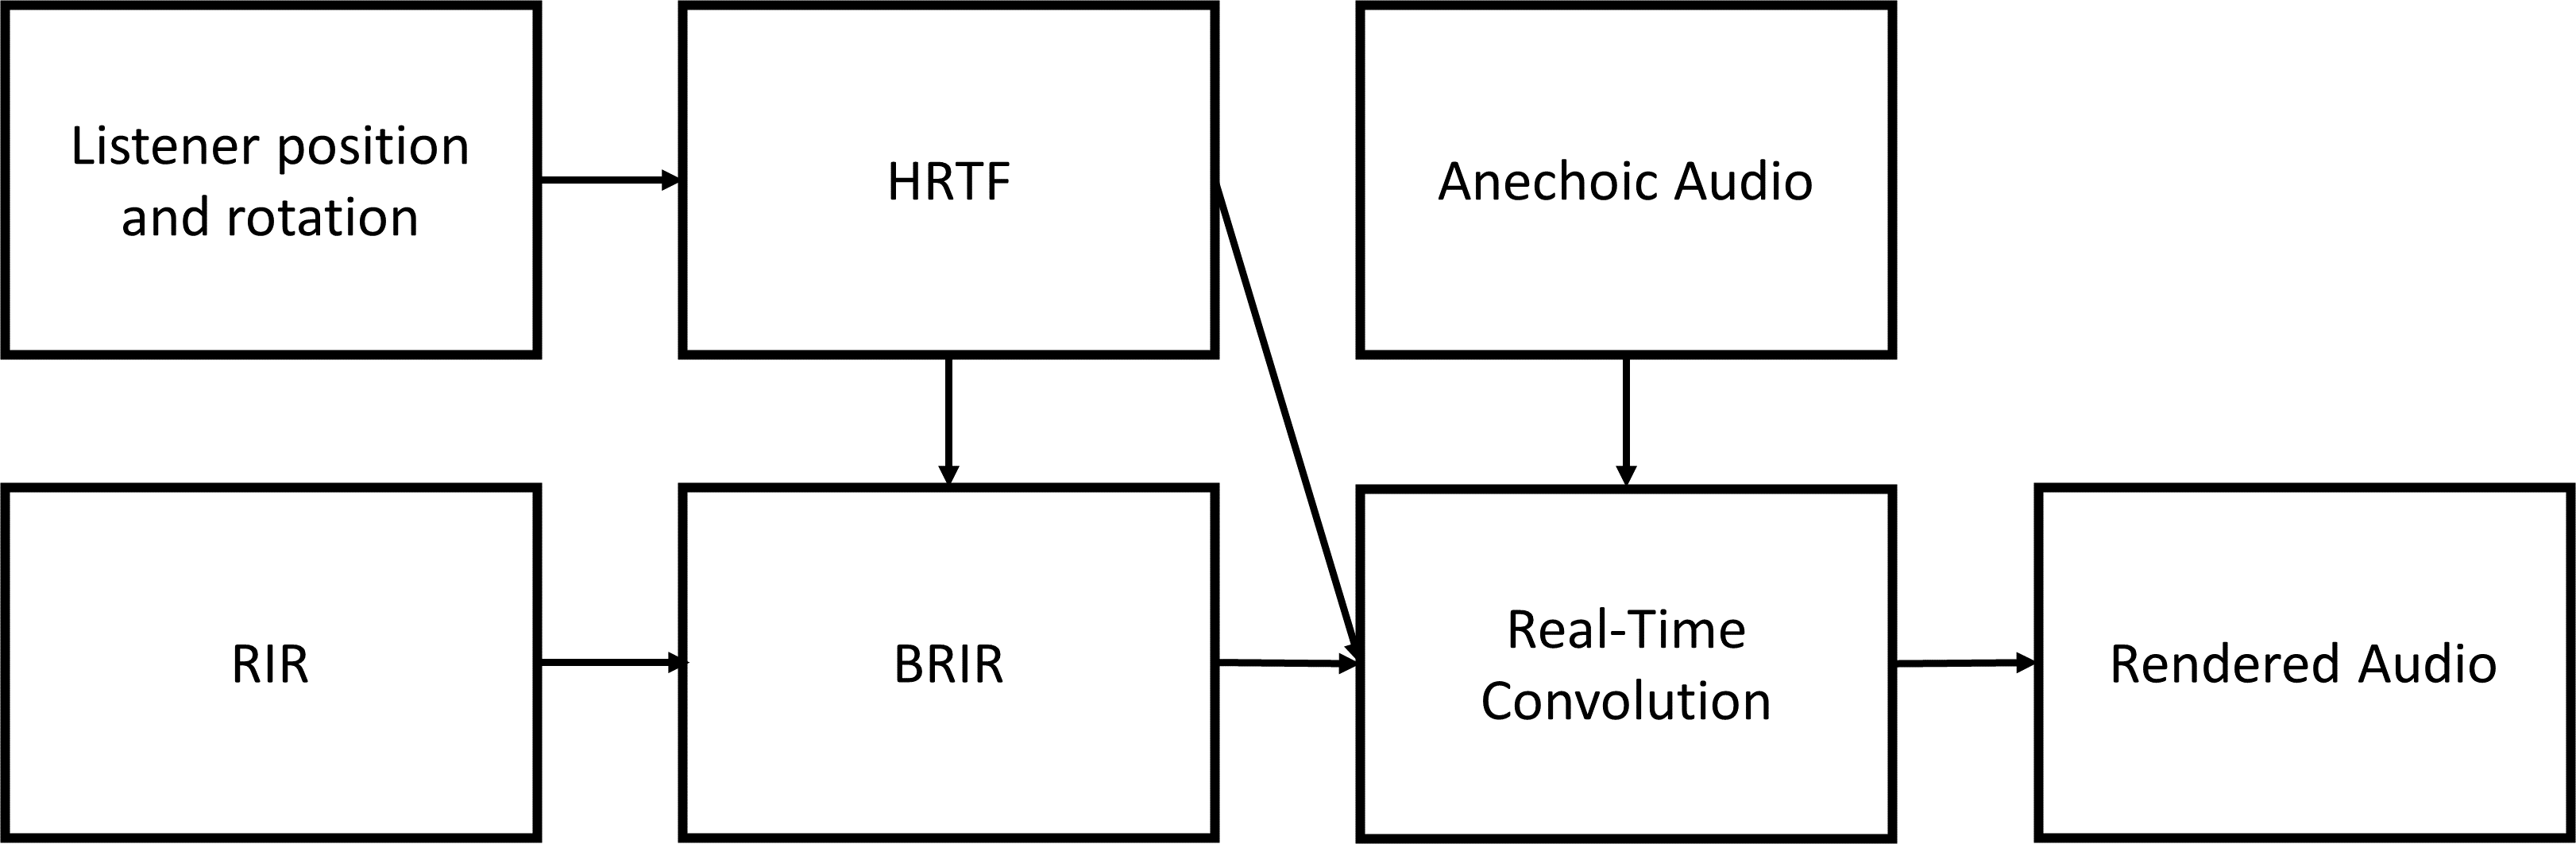
\includegraphics[width=1\textwidth]{audio_rendering}
    \caption{Common spatial audio pipeline: the listener's position and rotation in the scene is used to sample an interpolated HRTF from the currently loaded bank, combined with the generated IR, the real-time convolution algorithm applies the BRIR to an anechoic audio signal. The result is an audio signal arriving at the listener, taking into account their position and rotation with respect to the sound-emitting object in the virtual environment.}
    \label{fig:audio_rendering_chain}
\end{figure}

\section{Auralisations}
The ability to auralising anechoic acoustic signals is one of the fundamental objectives in the domains of acoustics for surveying techniques, acoustics for interactive applications, and acoustics in extended reality. As seen in Section~\ref{sec:DSP-background}, there are DSP techniques that allow the application of acoustic fingerprints onto audio recordings by treating the acoustics phenomena as measurable functions that can be convolved to digital signals, see Equation \ref{eq:1d-convolution}. In higher-level terms, auralisation is the process of experiencing audio stimuli in a simulated soundscape, which can be perceiving an orchestra in a digital representation of a church, approximating how room acoustics affect the sound transmission between the orchestra and the listener in the virtual space. There are factors associated with this process that determine how well the resulting signal is able to fool the listener's auditory system into believing that the auralisation is real. Realism and presence are often a function of the performance of the components in the chain of the 3D audio reproduction system; see Figure~\ref{fig:audio_rendering_chain}.

\subsection{Common methods for Auralisations}
Methods for producing auralisation start from the creation of an environment, which is the first component of the system in Figure~\ref{fig:audio_rendering_chain} hosting the virtual sound-emitting objects, e.g. an orchestra, and the virtual sound-receiving objects, e.g. the listener. In computers, environments are generally represented using a broad range of computer graphics techniques, from simplistic Computer-Aided Design (CAD) to fully-featured virtual worlds engineered in modern game engines. Such a statement blurs the definition of a virtual environment, as one could represent a room by creating a photorealistic 3D model or by simply drawing a cuboid. Research on acoustic simulations conducted over the last decades has expanded towards defining what is required from a virtual environment to produce a believable simulation. The representation of the environment geometry is a determinant of the resolution and perceptual quality of the acoustics simulation results, and, as a general rule, the higher the level of details expressed by the geometry, the more accurate the acoustic simulator is able to simulate how sound interacts with the environment. However, beyond certain levels of details, the increase in resolution does not have a significant perceptual response \cite{pelzer2010frequency}.\par
Combined with advances in real-space scanning technology and user-friendly 3D reconstruction software, it is now possible to create appropriate virtual environments for acoustic simulations without requiring expert computer graphics engineering knowledge.\par

\subsubsection{Geometrical Acoustics Modelling Techniques}\label{sec:bg-raytracing}
Geometrical acoustics is a family of acoustic modelling methods based on representing propagating sound waves with geometrical primitives, such as rays or cones. The foundations of these methods have sound propagating as straight lines, as opposed to moving particles, approximating the complex nature of acoustic energy transfer but neglecting phenomena related to the wave phenomena.

\citep{savioja2015overview}.

Ray-based techniques, wave-ray hybrid techniques, and wave-based techniques have emerged as prominent methods to generate impulse responses in the field of acoustics, each contributing to understanding how sound propagates within a given space. Ray-based techniques, rooted in geometric acoustics, simulate sound by tracing rays that emanate from a source and bounce off various surfaces within a space. This method creates echoes and reverberations, contributing to the overall impulse response. Notably, it offers efficiency as it is computationally less demanding than wave-based techniques, making it suitable for real-time applications or large-scale spaces often found in cultural heritage contexts. The geometrical nature of ray-based methods allows for easier integration with virtual reconstructions of space and dynamic geometry, and the method's inherent flexibility makes it easily adjustable to different acoustic scenarios. \cite{vorlander2008simulation}

\subsubsection{Hybrid Modelling Techniques}
On the other hand, wave-ray hybrid techniques present a more complex picture, combining aspects of ray-based and wave-based methods. Rays are utilised to model the high-frequency components of the sound, while wave equations handle the low-frequency behaviour, attempting to capture the best attributes of both methods. However, the hybrid nature often means more computational resources are needed, and it might not always be the most suitable choice for fast applications where platforms offer limited computational resources. \cite{hulusic2012acoustic}

\subsubsection{Wave-based Modelling Techniques}
Wave-based techniques stand out for their precision, solving the wave equation to simulate how sound waves propagate through space, accurately modelling diffraction, scattering, and other complex wave phenomena. While highly accurate, wave-based techniques often require substantial computational resources, making them less suited for real-time or large-scale applications. \cite{hamilton2017fdtd, raghuvanshi2014parametric}.\par

\subsubsection{Summary}
Ray-based techniques offer a compelling option for interactive applications. Their computational efficiency, relative simplicity, and adaptability in handling various scenarios effectively capture the essential acoustic characteristics of sounscapes. Unlike wave-based or hybrid methods, ray-based techniques can easily adapt to dynamic environments, aligning with the objectives of this work and constraints often found in \acrshort{ar} platforms. Therefore, while the high accuracy of wave-based methods or the comprehensive nature of hybrid methods may have specific applications in areas of high-fidelity and complex propagation effects, it is the ray-based techniques (such as those employed by acoustic simulation software such as ODEON) that generally stand out as the most appropriate choice for fast and efficient acoustic simulation in immersive applications.

% ---------------------------------------------------------------------------------
% * Virtual Environments
% ---------------------------------------------------------------------------------
\section{Virtual Environments}
Room acoustics simulations may involve the concept of virtual environments to represent sound-emitting objects, receivers, and space where these exist. Computer games technology has shaped the definition of virtual environments over decades of development and progress.

\subsection{Representation of Virtual Environments}
Graphics rendering pipelines display objects of a complex scene to viewers, determining the appearance of materials and geometry of the environment. In VEs, meshes are composed of triangles enabling game engines to organise geometry based on the semantics of scene objects. For E.g. a mug can be represented by triangles grouped in a mesh. They are essentially a network of triangles that connect, having adjacent vertices, to form objects. They are responsible for transforming the scene geometry and applying further processing, such as rasterisation, which generates fragments from geometry combined to create frames. A series of frames generated at interactive rates compose a frame buffer that allows users to experience scenes in real-time. Graphics pipelines describe geometry as vertices and triangles, applying shading techniques to control the appearance of surfaces depending on their lighting conditions and the viewer’s spatial position. Here, texture images can also define the appearance of objects' geometry by painting their surfaces and controlling transparency \citep{mcallister2002efficient, marschner2015fundamentals}.\par
Textures can determine the appearance of material composing objects in a scene adopting two-dimensional images. Texture mapping uses colour and transparency information contained in these images to paint triangles forming the geometry. Texture coordinates provide graphics pipelines with enough information to paint meshes.

\subsection{Handling of Complex Scene Geometry}\label{sec:bg-geometry-handling}
Implementing multimodal interactions in \ACRshortpl{ve} often requires handling and performing operations on the scene geometry, including searching interactions between entities and the environment. In computer games, physics systems are often fundamental components enabling game mechanics and interactions, which often involve computing intersections between scene entities and the environment. With the growing density of environment geometry and complexity of the scene elements, the computational requirements associated with evaluating these geometry searches have grown, demanding optimal solutions across the space and time domains.\par
The goal of geometry handling systems is to allow searching intersections between volumes or primitives, such as rays or frustums, and the scene geometry and the engineering design of such systems are closely related to data structures and algorithm design. Data structures space and time complexity
\begin{figure}
    \centering
    \begin{subfigure}[t]{0.3\textwidth}
       \centering
       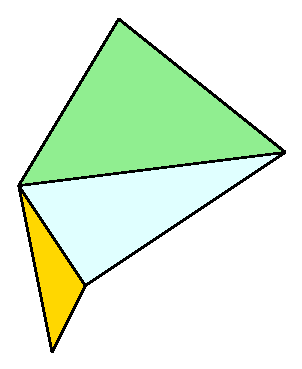
\includegraphics[width=\textwidth]{bvh1}
       \caption{Triangulated Mesh}\label{fig:sub_bvh1}
    \end{subfigure}
    \hfill
    \begin{subfigure}[t]{0.3\textwidth}
       \centering
       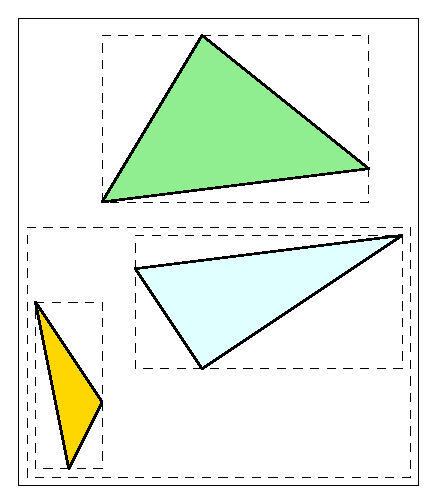
\includegraphics[width=\textwidth]{bvh2}
       \caption{Bounding Volumes}\label{fig:sub_bvh2}
    \end{subfigure}

    \begin{subfigure}[t]{0.8\textwidth}
        \centering
        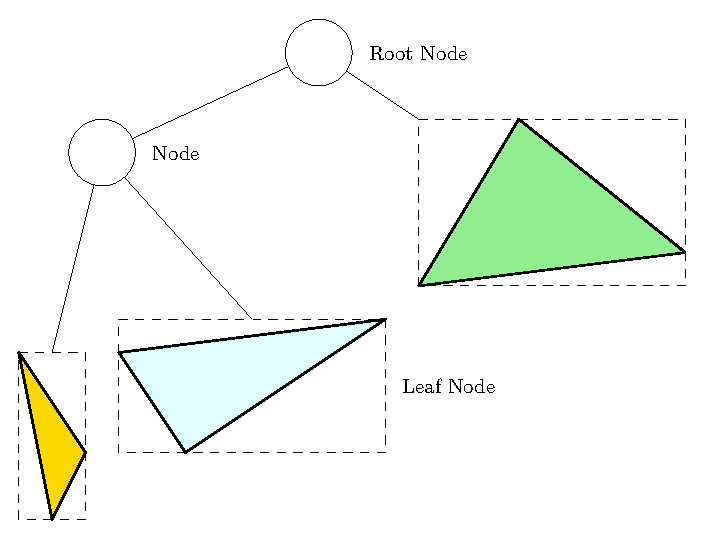
\includegraphics[width=\textwidth]{bvh3}
        \caption{Tree}\label{fig:sub_bvh3}
    \end{subfigure}
    \caption{A bounding volume hierarchy constructed on a given input scene represented as a triangulated mesh (a). Bounding volumes encapsulate mesh primitives, (b), which then represent nodes of the tree, (c).}\label{fig:bvh-diagram}
\end{figure}


\subsubsection{Binary Space Partitioning}
One of the first approaches in handling and indexing scene geometry in \acrshortpl{ve} is \acrfull{bsp}, which, motivated by performance aspects and limited computational resources available during the early developments of rendering pipelines in the field of computer graphics \citep{fuchs_bsp}. \acrshortpl{bsp} allow graphics pipelines to organise the order of scene elements before drawing them or to determine the visibility of surfaces.\par
The goal of \acrshortpl{bsp} is to index and search scene elements or geometry primitives, part of a given input scene. The technique works by subdividing the Euclidean space in which scene elements exist. The space is divided by partitioning planes, separating scene elements based on which side of the plane they exist. The process repeats recursively, subdividing space with further partitioning planes. Several criteria can determine the number of further subdivisions, such as the minimum size of regions generated by space subdivisions or the indexing complexity and granularity required for indexing and searching operations.\par
With subdivided regions obtained with partitioning planes, a binary tree, similar to the diagram shown in Figure~\ref{fig:bvh-diagram}, where a root node refers to the entire scene and branches into the first space subdivision, which recursively branches into further subdivisions, until a ``leaf'' region. A leaf region can hold a scene element, a geometry primitive, or a subset of primitives from the set of primitives representing the input scene.\par

\subsubsection{Bounding Volume Hierarchies}
A \acrfull{bvh} is a method closely related to \acrshort{bsp} for handling scene geometry that optimises intersections between rays and the scene by adopting a binary tree to subdivide primitives that compose the scene geometry. A \acrshort{bvh} can represent a scene by constructing a binary tree partitioning geometry primitives into a hierarchy of disjoint sets. In physically-based rendering applications, mesh triangles are often the primitives indexed by the constructed tree; see Figure~\ref{fig:bvh-diagram} \citep{pharr2023physically}.\par
In a tree, bounding volumes are generated to fit primitives from a given triangulated mesh (Figure~\ref{fig:sub_bvh1}) and aggregated based on proximity (Figure~\ref{fig:sub_bvh2}). Bounding volumes encapsulating multiple primitives generate branches, and recursively, branches are encapsulated in volume until a root volume fits the entire input scene. A constructed tree (Figure~\ref{fig:sub_bvh3}) can be queried and traversed by navigating branches from the root node to primitives within leaf nodes.\par
Thanks to branch subdivisions, ray-volume intersection tests performed on nodes allow filtering out entire segments of the scene, reducing the set of primitives that potentially intersect the ray to a subset of the input scene triangle set and improving the space complexity of the operation, much like in \acrshort{bsp} techniques. Recent research trends are exploring tree rotations and balancing of branches in real-time, optimising search operations even further, and allowing the tree to reflect dynamic changes to the scene geometry \citep{kopta2012fast}.
 
\subsection{Sound Sources in Virtual Environments}
Representing space in virtual environments, capturing real space and synthetic scenes.
- Game Engine architecture book                             

\subsection{Materials}
\begin{figure}
    \centering
    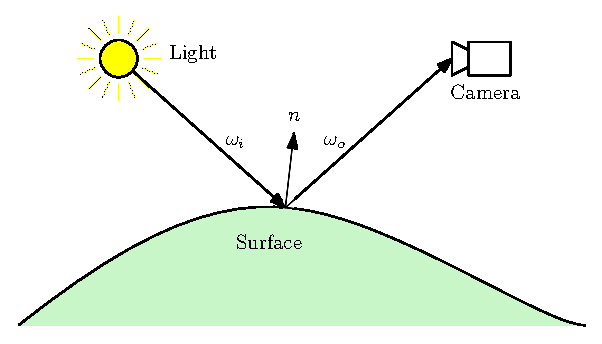
\includegraphics[width=1\textwidth]{brdf1}
    \caption{A simplistic material system visualised as a ray of light emitted by a source and colliding with a surface. The ray reflects around a surface normal and is detected by a virtual camera.}\label{fig:material-vis}
\end{figure}
In computer graphics and multi-modal rendering, assigning physical properties to surfaces of the scene geometry has been addressed with the definition of materials. The definition of materials is often intrinsic to the rendering technique and to the engineering design of the rendering apparatus. In physically-based graphics rendering techniques,~\cite{pharr2023physically} define materials as a
\begin{quotation}
    ``description of its appearance properties at each point on the surface''.
\end{quotation}
\subsubsection{Materials in Rendering Pipelines}
Rendering pipelines often model how surfaces in complex scenes reflect and respond to propagating energy by employing \acrfullpl{brdf}. In the light domain, rendering techniques often model reflected energy as a function $f_r(p, \omega_i, \omega_o)$ of a $p$ \acrshort{brdf}, an incoming direction $\omega_i$ and an outgoing direction $\omega_o$. A simplified diagram in Figure~\ref{fig:material-vis} shows how energy transmits from a light source and is sampled by a virtual camera, with a surface reflecting the light ray around the surface normal at the collision point. Though, materials in the real world have unique physical properties affecting reflectance, absorptions, or diffusion of incidental light, deviating from the idealised model shown in the Figure.\par
A material using a reflectance function can model realistic behaviour, allowing surfaces to express varying physical attributes like roughness or metallic characteristics. Figure~\ref{fig:brdf-vis} shows example functions simulating a rough and a glossy material, Figure~\ref{fig:brdf1}~and~\ref{fig:brdf2} respectively. These examples show \acrshortpl{brdf} modelling the scattering of energy caused by the rough surface and the glossy reflections caused by a mirror-like surface.\par
\subsubsection{Materials in Sound Rendering}
Defining materials translates to the acoustics domain, applying closely related principles defined in the visual domain. \ACRshort{ga} methods often share the same approach shown in Figure~\ref{fig:material-vis} by considering sound in \acrshortpl{ve} as propagating rays (or other geometry primitives) colliding with surfaces that reflect energy based on attributes assigned to the surface.\par
In real soundfields, acousticians and architects often plan the presence of certain materials to control aspects of sound propagation within a given environment. Studies show that strategic placements of surfaces with high acoustic absorption characteristics can have a positive subjective influence on perception in environments, improving the clarity of acoustic information transmitted within the space \citep{arvidsson2021subjective}. Absorption panels, diffusers, or bass traps are some example materials and surfaces that acousticians use to control how acoustic energy reflects around the environment, controlling parameters like $T_{30}$ or $T_{60}$ reverberation metrics or $C_{50}$ and $D_{50}$ clarity and definition metrics, respectively.\par
Modern game engines and acoustic simulation software aim to replicate the behaviour of these surfaces by encoding acoustic characteristics to scene geometry representing an environment. In \acrshort{ga} simulation methods, material characteristics like absorption or scattering coefficients can influence of geometry primitive simulating propagating sound and interact with the environment, similarly to \acrshortpl{brdf} \citep{rindel2000use}. Finally, acoustic material can encode frequency-dependent acoustic information, often expressed around \acrfull{erb} frequency region, to consider aspects of the \acrshort{has}. Chapters~\ref{ch:Materials}~and~\ref{ch:acousticrendering} will discuss the use of materials in the context of the overarching aim of this thesis.

\begin{figure}
  \centering
    \begin{subfigure}[t]{0.49\textwidth}
       \centering
       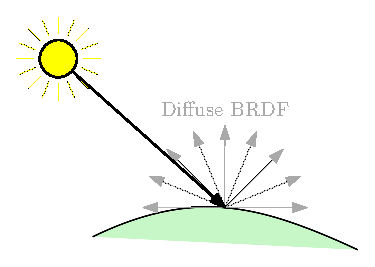
\includegraphics[width=\textwidth]{brdf2}
       \caption{Rough Material}\label{fig:brdf1}
    \end{subfigure}
  \hfill
    \begin{subfigure}[t]{0.49\textwidth}
       \centering
       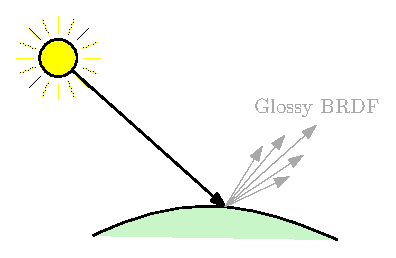
\includegraphics[width=\textwidth]{brdf3}
       \caption{Glossy Material}\label{fig:brdf2}
    \end{subfigure}
  \caption{Example \acrshortpl{brdf} applied to a surface, defining a rough material (a) and glossy material (b). These functions emulate how properties of real surfaces respond to colliding light: glossy materials will reflect energy specularly, whereas uneven rough surfaces will cause diffuse scattering.}\label{fig:brdf-vis}
\end{figure}

% Absorption, diffusion, scattering, and physical properties of materials.

\section{Deep Learning}
Subsequent chapters of this thesis will leverage deep learning techniques to solve a subset of problems associated with developing a system targeting the overarching aim. Specifically, acoustic materials are central to applying the system to realistic, complex scenes, as they contribute towards the perceived quality and realism evoked by the auditory display. The problem arises from the complexity of mapping the appearance of surfaces within the complex scene to acoustic materials. Many factors in complex virtual environments influence the appearance of surfaces, making it hard to distinguish surfaces and map them against acoustic materials automatically.\par
Deep learning is a subset of machine learning comprising techniques and pipelines to address such mapping problems by learning from examples and providing a generalised model for unseen cases. The potential of deep learning lies in the feature extraction process, allowing models to learn from examples influenced by many factors. The term deep learning is associated with the feature extraction process, delegated to layered feature extraction components composing the model.\par
The goal of a model is to provide inference on unseen data based on training on a set of representative examples, emulating basic human abilities that are hard to programmatically engineer in computers.

\begin{figure}
    \centering
    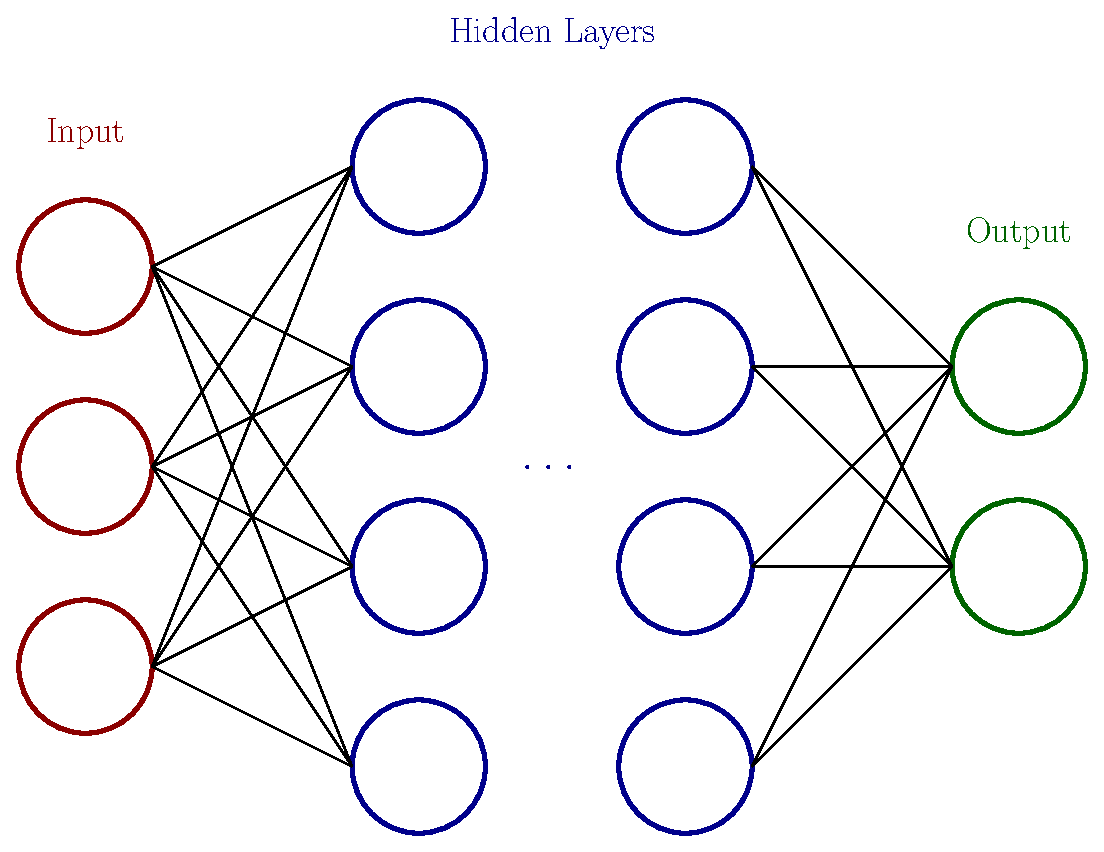
\includegraphics[width=1\textwidth]{nn}
    \caption{A visualisation of a basic neural network with fully-connected hidden layers.}\label{fig:nn}
\end{figure}

\cite{goodfellow2016deep}
General Machine Learning Tasks

\begin{itemize}
    \item classification
    \item regression
    \item synthesis and sampling
    \item extrapolation
\end{itemize}

TPUs and specialised hardware for neural nets.

\subsection{Applications Within Immersive Media}
Deep learning techniques are becoming increasingly popular in virtual environment pipelines due to the flexibility and potential to adapt to various tasks. 

\subsection{Object Detection and Segmentation}
Detecting the presence of certain objects in an image represents a milestone in the development of \acrshortpl{cnn} and computer vision techniques as it emulates a basic task of the human visual system. Due to the nature of image representations in computers, as described in Section~\ref{sec:image-processing}, recognising entities depicted by images is a central problem in computer vision \citep{szeliski2022computer}. Classic computer vision algorithms have approached the problem by providing algorithms to recognise patterns programmatically by filtering the image or scanning for certain features. Thanks to advances in \acrshortpl{cnn}, object detection was addressed by extracting features using deep layers and learning from annotated examples expressing a set of classes captured in various contexts.\par
Pioneering large-scale labelled datasets, such as the work by~\cite{deng2009imagenet} on ImageNet, enabled object detection networks to improve their efficiency and abilities of recognising classes. Of pioneering importance is~\cite{Redmon_2016_CVPR}'s You Only Look Once (YOLO) network that introduced a state-of-the-art solution able to recognise thousands of classes with high accuracy and precision.

Similarly to object detection, the problem of image segmentation \cite{minae_segmentation} (review of techniques)


\begin{itemize}
    \item 3D scene segmentation and recognition \cite{kalogerakis20173d}
    \item pose estimation \cite{andriluka20142d}
    \item scene reconstruction \cite{patow2003survey}
    \item sound source separation \cite{virtanen2006sound}
    \item audio scene understanding \cite{abesser2020review}
    \item sound propagation \cite{liu2022sound}
    \item perceptual similarity \cite{Dolhasz_2020_CVPR}
    \item agency in games \cite{yannakakis2018artificial}
\end{itemize}

\subsection{Audio Scene Understanding and Source Separation}
Reasoning and performing tasks on auditory information are analogous to computer vision problems due to the same nature of digital representations.

Sound source separation, also known as audio source separation or audio source separation, is a process in audio signal processing that aims to separate individual sound sources from a mixture of sounds. It is the task of isolating and extracting specific audio sources from a recording where multiple sound sources are present. In many real-world scenarios, such as music recordings, conversations, or environmental recordings, multiple sound sources contribute to the overall audio signal. Sound source separation techniques are employed to enhance the clarity and quality of individual sources, making it easier to analyze, process, or manipulate specific elements within the audio.

\section{Conclusions}

The current state of interactive sound rendering allows for fast acoustic simulations, even on platforms with limited computational budgets, approximating the soundfield of any given environment, where a listener can experience realistic auditory interactions with virtual sound sources \citep{lakka2018spatial, hulusic2012acoustic}. Sound rendering can be considered a fundamental component of computer games technology, responsible for reproducing everyday sound emitted by objects or agents in a virtual scene and perceived by a listener. This poses the challenging task of reflecting basic acoustic principles to render such auditory interactions realistic. In the real world, sound propagates from a sound source to a listener and interacts with objects in the environment and with the environment itself arriving at the listener's ears \citep{kuttruff2016room}. Sound cues alone are sufficient to enable users in Virtual Environments (VEs) to pinpoint locations of sound-emitting entities in a scene by using auditory sound localisation, a natural ability associated with the human auditory system \citep{lokki2005navigation, rubio2017immersive}. \par
As the acoustic principles that govern how sound propagates in space are difficult to reproduce in digital systems, many methods exist, providing variable orders of approximations, depending on the application. Such approaches emulate the wavefield of an environment, simulating how sound interacts with boundaries and scene objects. A subset of these can reproduce phenomena of sound, such as diffraction, reflection, and refraction, which are determinants of realism as they emulate how waves bend around obstacles. Such phenomena make the simulated wavefield dependent on the accuracy of scene geometry and materials represented in a VE. \par
There is a large tree of techniques and methods to simulate sound propagation, reflecting acoustic properties to any given sound source in a VE, adapting to perceptual requirements and computational budgets available \cite{doukakis2019audio}. As a general rule, the more computational budget available, the more complex techniques can be employed, allowing realistic sound rendering. Finite-difference Time Domain (FDTD) approaches shown by \cite{hamilton2017fdtd}, or wave-based by~\cite{raghuvanshi2014parametric} methods, on this end of the spectrum, obtain high degrees of accuracy and realism, but often require pre-computation stages or GPU implementations to produce acoustic simulations at interactive rates. On the other end of the spectrum, there are fast geometrical acoustics methods, widely adopted in real-time applications due to their low computational requirements and highly parallelisable implementations \citep{cowan2010gpu}, which reduce simulated sound waves to rays or beams, that are much simpler to compute. Finally, hybrid methods also exist to combine the strengths of the main families. \par
Acousticians and engineers have always employed classic sound rendering to solve practical problems as it requires the work of experts to adjust parameters and define the acoustic characteristics of a virtual scene. A constant here is the requirement of an accurate description of the environment, detailing the geometry of architectural components and objects contained within with acoustic information such as acoustic energy absorption, reflection, or scattering --- this is essential to model the behaviour of sound waves interacting with the environment. \par
Only recently, with the increase of processing power available in computers, it has gained popularity in computer games and immersive technology for entertainment and serious applications \citep{zhang18}. Augmented Reality (AR) technology can particularly benefit from this as the increase in processing allows sound rendering on mobile devices, enabling listeners to experience virtual sound sources propagating in the reconstruction of real geometry, which is the main avenue that the planned thesis work aims to explore. \par

% Acoustic materials
% Deep learning for acoustic materials
% Next up: lit review





% \chapter{Literature Review}\label{ch:litReview}% TODO Introduce each area properly
In light of the grounding provided around the domains of wave theory, digital signal processing, acoustics and soundfield simulations, as well as domains of computer graphics and vision, virtual environments, and immersive displays, this Chapter reviews the current state of research overlapping the primary aim of the thesis. Throughout this work, the thesis objectives may be reiterated to provide the reader with context relative to the Chapter or Section at hand. The overarching goal of this work is to explore the potential of computer vision within acoustic rendering pipelines for realistic sound transmissions between virtual sound-emitting objects perceived by a user in a virtual environment.\par
This Chapter gathers pioneering work, state-of-the-art, and experimental methods to address problems or tasks associated with each component of the thesis aim. Methods and experiments are reviewed, considering limitations and expansion points to inform design choices in engineering systems proposed throughout the following Chapters. Discussions around existing work aim at both orienting the reader towards the goal of each domain associated with the thesis component and defining the value of the contributions stemming from this work.\par

\section{Introduction}
The vision for augmented reality, ISMAR keynote.
The current state of interactive sound rendering
Emerging technology of space sensing
\cite{yang2022audio} audio interactions, removing unwanted noises from the augmented scene. Research towards multi-modal interactions has seen decades of advances INCLUDE REFS The field of Audio Augmented Reality (AAR) 
% Introduce virtual environments


\section{AAR: Audio Augmented Reality}
ref: Spatialised Audio Rendering for Immersive Virtual Environment]
The authors present a novel architecture for spatialised audio rendering for virtual environments experienced through immersive headsets. They define 3D sound localisation, room simulation, live audio input and efficiency as the main requirements the architecture should feature. The architecture draws from low-level rendering pipelines, such as graphic sub-systems, to integrate sound rendering procedures into existing scene-handling systems adopted by these pipelines. 


\section{Visual-Acoustic Mappings}\label{sec:lr-visual-acoustic-mapping}

Methods have been proposed to map visual representations of environments to their acoustic features. Sound rendering in virtual environments can leverage such mapping for producing audio stimuli conveying spatial information to the user. Recent work solves tasks within sound rendering for virtual environments, such as propagating audio within virtual environments. 
Spatial sound has been shown to be influential in having a significant effect on the sense of presence and immersion for a user in a VE \cite{poeschl13}. Factors of accurate and plausible acoustic rendering include geometry, material definitions and a room impulse response which describes the attenuation of sound from a sound source to a listener, and there exist approaches that tackle varying aspects of these factors.
A common denominator in the sound rendering methods mentioned is the problem of mapping visual representation of environments to corresponding acoustic materials, which intersects image processing and computer vision domains aimed at modelling how human vision recognise materials.\par%

\subsection{Modern Sound Rendering}
In Virtual Environments (VEs), acoustic rendering can reproduce spatial hearing abilities \cite{lokki2005navigation}, supporting architectural acoustics, cultural heritage \cite{berardi2016acoustic, vorlander2015virtual}, and computer games \cite{raghuvanshi2014parametric, mehra2015wave} to build compelling, realistic acoustic simulations. Recent advances in wavefield synthesis have made it easier and computationally feasible to apply to VEs~\cite{raghuvanshi2014parametric}. They draw on geometrical acoustics, wave-based or hybrid sound propagation algorithms, simulating sound propagation by tracing rays or beams \cite{hulusic2012acoustic}; solving the wave equations at discretised junctures of the representation of the environment or by a combination of the former techniques. They enable game designers to apply realistic, spatialised audio to games.

In acoustics, it is common to capture an environment adopting measurement techniques such as the sine sweep, usually consisting of reproducing a logarithm sine chirp or a short burst, e.g. a gunshot,  emulating a Dirac-delta function to excite frequencies in the audible spectrum and recording how the environment influenced the propagated sound at the listener position \cite{reilly1995convolution}. Such measurements can determine a Room Impulse Response (RIR), a series of reflection paths over time, recreating the acoustic space for a given source-listener position pair. Wave-based acoustic simulations achieve the highest degrees of realism in generating acoustic fields as they compute sound propagation via simulations of high-dimensional pressure fields \cite{raghuvanshi2014parametric} or solving the wave equation with Finite-Difference Time-Domain schemes \cite{hamilton2017fdtd}. Their inherently complex nature require solving the wave equation to produce acoustic simulations for a given scene, and despite recent GPU-based solvers optimising complexity by orders of magnitude \cite{mehra2012efficient}. Their computational requirements are often impractical for real-time applications due to the nature of the wave equation, resulting in numerical complexity increases with frequency. On the other end of the spectrum, Geometrical Acoustics (GA) provide methods for fast approximations of acoustic space; they have gained popularity among extended reality platforms due to their highly parallelisable implementations \cite{savioja2015overview}.\par
Schissler and Manocha \cite{schissler2016interactive} introduced an acoustic rendering system based on ray-tracing, adapting to large complex scenes. Among their contributions is overcoming the problem of handling many sound sources in large-scale environments by clustering them based on the distance from the listener. Based on an octree representation of space, with respect to the listener position, their clustering aggregates increasing numbers of sources as their distance from the listener increases. Their approach highlights the need for dissecting the acoustic space for efficient selective rendering, resulting in rendering of fine perceptual details within the listener's close proximity and coarse approximations otherwise. \par

Schissler \textit{et al.} \cite{schissler2021fast} recently presented a novel method for computing acoustic diffraction in real-time, which can adapt to GA frameworks. They target complex scenes typical of virtual and augmented reality applications. Their approach can overcome the inability of GA techniques to simulate phenomena intrinsic to waves.\par

\subsection{Experimental Methods for Sound Rendering}
Tang \textit{et al.} \cite{manocha2020differentiable} present a model for simulating sound fields using neural networks without pre-computing the wave field of an acoustic environment, predicting unseen objects with arbitrary shapes in a VE for sound propagation at interactive rates. They train a geometrical neural network on annotated meshes to infer acoustic data associated with the represented object.
\cite{chen2022visual} introduce a novel task dependant on this mapping, \textit{visual/acoustic matching}, which produces acoustic stimuli responding to a target space depicted in an image, given an input audio excerpt and an image of the environment in which excerpt propagated. The rapid development in DNN for multi-modal applications has opened new avenues in the field of sound propagation modelling, one of which tapped into visual-acoustic mapping, the process of determining relationships between visual and auditory features in audio-visual or immersive media.\par
One pioneering experiment,~\cite{Singh_2021_ICCV}'s Image2Reverb, towards this unexplored avenue used a DNN to define mappings between images and reverberation, expressed as an RIR. By observing photographs of real or virtual environments, our visual system is generally able to infer acoustic characteristics of the space; from a photograph of a cathedral, for instance, we can imagine its reverberant aural footprint. The authors aimed to leverage CNNs and GANs to explore automated mappings between deep visual features extracted from a given input image, representing an environment, and an output spectrogram of an RIR. Since many reverb metrics like the $T_{60}$ are linearly correlated to the energy decay in RIRs, their network encodes reverb by representing a spectrogram with variable energy decay. The authors train and evaluate the network by comparing results to ground truths pairs of photographs and measured responses, achieving around $0.87s$ mean error in $T_{60}$ estimations.\par
Improvements and new approaches to solving the task are being explored at increasing rates, such as~\cite{somayazulu2023self}'s network presenting a self-supervised visual-acoustic matching system. With an input audio excerpt and a target image representing an environment, their system re-synthesises the audio excerpt to reflect the acoustic features of the target environment. A key novel aspect of their method is the handling of reverberant audio by leveraging a state-of-the-art network for audio dereverberation (which is a well-established task in the field of acoustic signal processing). The de-reverberated audio is passed to a GAN, which optimises the output audio until it acoustically matches the extracted visual features.\par

\cite{liang2023neural} present a method that improves on the adoption of Neural Radiance Fields for sound propagation. The authors present a method that allows a neural field to be learned on a real soundscape by providing emitter and receiver position input, a ground truth RIR, and acoustic context representations. The neural field fit on the input environment allows the generation of novel RIRs based on given emitter-receiver position pairs. The neural field learns from multimodal representations of the environment, expressed as visual information by RGB + depth images and acoustic data by emitter-receiver position information.\par

\cite{tang2020scene} present a novel scene-aware sound rendering system aimed at rendering audio considering acoustic characteristics of a given room, providing real-time audio effects applied to novel signal matching the soundscape of the input room. The system uses a neural network to infer reverberation time and estimate resonance interferences caused by the room architecture using a recorded signal and 3D representation of the environment where the recording is generated. Their method uses the inferred acoustic properties as input to an acoustic simulator that generates and optimises acoustic materials by measuring simulation errors against the estimated room features. Once the acoustic simulator optimises materials, it convolves IRs with novel audio signals to emulate a sound source propagating in the input environment. As part of the testing procedures, the authors provide a benchmark for the material optimisation pipeline, outlining the error in estimated materials across rooms of increasing reverberation times; it increases with the size of the input room. Their system provides realistic acoustic stimuli as subjective tests show that the simulation error is not perceptually significant.\par

\cite{chen2023everywhere} use Audio-Visual receivers to sample reference features, generating joint audio-visual representations of input scenes to synthesise novel binaural audio. Their system takes visual information and uses a Joint Audio-Visual Representation to extract audio-visual features from space, which feed into an Integrated Rendering Head. The rendering head uses a ground-truth binaural waveform to optimise output binaural audio generated given a listener position. Their rendering pipeline improves state-of-the-art methods, such as few-shots learning-based techniques for sound rendering, by evaluating simulations on standard acoustic scenes and indoor space reconstruction datasets.\par

\cite{ratnarajah2022mesh2ir} present the first approach to neural networks for sound rendering.

Yang \textit{et al.} \cite{yang2020fast} present a method for synthesising Room Impulse Responses (RIRs), reproducing perceptually-convincing acoustics of real environments based on a small number of ultrasonic measurements.\par
Li \textit{et al.} \cite{li2018scene} identify a novel method for acoustic simulations using convolutional neural networks to perform acoustic analysis on videos, veering away from more formal 3D scene definition. This approach synthesises RIRs for environments' representations from audio-visual scenes. Their system extracts high-level acoustic properties such as reverberation time T\textsubscript{60} and frequency-dependent amplitude level (EQ).\par

% Please add the following required packages to your document preamble:
% \usepackage{booktabs}
\begin{table}[]
\centering
\begin{tabular}{@{}llllll@{}}
\toprule
Method                       & Task                 & Architecture & Inputs              & Requirements        & Notes                                                          \\ \midrule
\cite{Singh_2021_ICCV}       & Reverb apprx.        & GAN          & RGB image           & DNN forward pass   & Efficient. No consideration for source-emitter receiver.       \\
\cite{ratnarajah2022mesh2ir} & RIR estimation       & Graph NN     & S-R, 3D Mesh        & DNN forward pass   & 10.000 IR per second. Limited control over acoustic materials. \\
\cite{liang2023neural}       & RIR query            & NAF          & S-R, RGBD data      & NAF query          & Fast and highly generalisable.                                 \\ \bottomrule
\end{tabular}
\caption{Summary of cutting-edge visual-acoustic mapping methods for sound propagation tasks in virtual environments. Glossary: GAN $\leftarrow$ Generative Adversarial Network; S-R pos. $\leftarrow$ source-receiver position information;  NAF $\leftarrow$ Neural Acoustic Field.}
\label{tab:visual-acoustic-mapping}
\end{table}

\section{Material Recognition for Rendering Tasks}
\cite{schissler2017acoustic} present a two-stage system for sound rendering based on scene understanding performance on scans of physical space, requiring reconstruction of physical space and acoustic measurements as input and, leveraging recent advances in semantic segmentation for audio-visual rendering tasks. The first stage of the system uses multiple camera viewpoints to reconstruct a dense 3D triangle mesh representing the environment and generate input to a CNN to classify acoustic materials from camera renders. A Least Square Solver algorithm uses real measurements to optimise the inferred materials by calculating the distance from estimated IRs to the ground-truth IRs.\par
Semantic segmentation tasks aim to assign a semantic class label to every pixel in the input image. Examples of applications in scene understanding include PixelNet \cite{bansal2016pixelnet}, which performs semantic segmentation and edge detection; EdgeNet \cite{dourado2019edgenet}, which combines depth information with semantic scene completion, using RGB-D input data. For synthetic data generation, UnrealCV provides a pipeline that generates images from VEs providing semantic segmentations \cite{qiu2016unrealcv}, allowing for easy generation of training data.
Large-scale datasets, including semantic and 3D information, have been released, e.g. the Matterport3D dataset \cite{chang2017matterport3d}, which provides panoramic images generated across real environments. 
Various domain-specific applications of these methods have been proposed, e.g. in mixed and augmented reality \cite{chen2018context}, where semantic information about surfaces can guide contextual interactions between virtual elements and real-world structures; or surveillance \cite{mao2018aic2018}, where the semantics of objects in the scene determine its subsequent processing. 
However, few examples of applying computer vision to realistic audio rendering exist. One approach \cite{kim2019immersive} uses $360^{\circ}$ photographs and depth estimates to generate 3D geometry and semantic information, which is then used for physically-based audio rendering and can also adapt to VEs. In this context, even approximate semantic information could allow for gains in efficiency and a decrease in the costs of applying physically-based audio rendering to VEs.

Recent developments in deep learning techniques have contributed to a dramatic increase in accuracy in tasks such as image classification. Specifically, convolutional neural networks have been broadly adopted to learning functions mapping between image data and various semantic descriptors, such as local object classes \cite{long2015fully}, perceptual sensitivity \cite{Dolhasz_2020_CVPR}, or subjective quality \cite{bosse2017deep}. For example, Lagunas \textit{et al.} \cite{lagunas2019similarity}, present a method to learn similarities between materials based on their appearance and distinguish them in a feature space, informed by human perception. They describe mappings between subjective perception and physical material parameters. This is a challenging task due to the impact of low-level properties, such as illumination and reflectance on the appearance of materials. The authors address this problem using deep features learned by a neural network trained on a bespoke dataset, annotated with around about 100 classes of materials, captured under different conditions, including surface shape, illuminance and reflectance, expressed by environment maps and bidirectional reflectance distribution functions. In a subjective study they encode materials in a perceptually-informed feature space, allowing for calculation of perceptual distances.\par
Schwartz and Nishino \cite{schwartz2019recognizing}, address the problem of material recognition from local visual information of materials to better model human interaction. They aim to reduce manual supervision in the process of encoding material characteristics, explaining visual attributes such as shiny or metallic and material properties that may not be visually or locally discoverable such as softness. They present a novel method for material recognition consisting of perceptually-informed distances between materials and attribute spaces based on the distances.
Semi-supervised approaches have also been adopted in tackling such problems. For example, Gaur and Manjunath \cite{gaur2019superpixel} propose a novel deep learning architecture to cluster materials from a given dataset, improving state-of-the-art superpixel algorithms by combining segmentation of images into perceptually meaningful pixel clusters with a novel unsupervised clustering method based on superpixel embeddings. A novel loss function uses a variable-margin that compensates the limitations of classic superpixel algorithms in segmenting texture patterns, allowing the convolutional neural network to cluster superpixel labels based on their embeddings requiring no manual supervision or annotations.\par%

Approaches like these have demonstrated the efficacy of deep learning techniques for learning complex nonlinear mappings directly from annotated image data. This work leverages and adapts such techniques for the purpose of local material classification, allowing for the first step in mapping from image features to acoustic absorption coefficients.

\subsection{Findings and Limitations}
CNNs are becoming optimised enough that can be embedded in real-time systems. Generalising on surfaces is still an open problem in the research domain.
A crucial finding within this area derives from \cite{schissler2017acoustic}, who pioneered the field of scene understanding systems for sound rendering, projecting these into use cases for multi-modal AR and identifying limitations that future work should address to be around improved material recognition and inference on outdoor scenes. In general, the problem of recognising materials both in physical and virtual environments remains an open research question within these domains due to the challenging task of associating semantics to the visual appearance of surfaces in complex scenes, which depends on factors associated with the physical properties of surfaces or lighting conditions.  

\section{Perceptually-informed Rendering and Human Factors in Audio-Visual Rendering}
\cite{bonneel2010bimodal}'s pioneering study investigates the influence of audio-visual stimuli, as well as the interaction of graphics and audio, on material perception. They designed an experiment testing whether graphics and audio have significant effects on the subjective perception of material qualities. Their 

\cite{slater2009visual} Realistic rendering affects presence and interactions

\subsection{Findings and Limitations}
Cross-modal interactions within VEs are generated from representations of entities that are consumed by rendering algorithms to produce audio-visual stimuli. 


\section{Psychoacoustic Factors in Sound Rendering}
\cite{gonzalez2023binaural}

\subsection{Perception of Audio Quality}
\cite{rummukainen2018audio} pioneered the field of audio quality evaluation in immersive technology by porting MUSHRA-like testing to VR platforms, evaluating the impact of audio engines in interactive multi-modal VEs. The MUlti-Stimulus ranking test with Hidden Reference and Anchor (MUSHRA), described in the International Standard ITU-R BS.1534, is a standard approach for evaluating the perceived audio quality of a system, often employed to evaluate coding, compression or processing tasks in the audio domain \cite{series2014method}. Thanks to \cite{waet2015}'s web implementations, MUSHRA methods have been providing an essential tool for A/B comparisons or audio effects or algorithms and can be used to evaluate the quality of acoustic phenomena simulated with rendering techniques, such as reverberation, echo, diffraction or other soundscape characteristics that can be encoded in RIRs.\par
\cite{rummukainen2018audio}'s framework gives MUSHRA methods new dimensions in VR scenarios, enabling the evaluation of renderer or spatialiser systems such as HRTF spatialisers. The VR nature of the framework can provide a wide breadth of metrics associated with the interaction between the listener, sound-emitting entities, the environment and tasks or procedures. The user study the authors conducted demonstrates how these metrics can provide further insights into perceptive aspects, for instance, showing how participants dwelled around testing areas during the execution of the procedure. With modern HMDs providing more and better interaction and sensing technology, researchers have access to eye, head or hand-tracking data, as well as more information regarding scene elements of the VE. Such data is generally unexplored, and investigation should explore how acoustic renderers affect subjective responses to audio stimuli.\par

\subsection{Psychoacoustic Characterisation of Sound Propagation Methods}
With the human listener as the central and final link in the chain of a sound rendering system, it is essential to consider how the audio display presented to the listener is affected by aspects related to human perception and psychoacoustic abilities performed by the HAS. Due to the applications of sound rendering in VEs within serious and entertainment domains, researchers often base subjective evaluations of sound rendering techniques on task performance, studying how sound rendering techniques affect interactions, navigation, localisation or other activities influenced by the hearing sense. \par
\cite{mehra2015wave} presented a novel, wave-based sound rendering technique aimed at VR applications, advancing the domain of particle simulations for interactive sound rendering. One of the key contributions of their approach is providing a system offering realistic sound propagation between moving sound sources and listeners and can adapt to large, complex scenes. Their system offers spatial audio reproduction based on head tracking features of HMDs and position information of the listener in the VE. The inherent limitation of their approach is the required pre-computation stage for evaluating acoustic energy transfers between geometry and objects in order to solve particle equations and generate the wave propagation field that can then be solved at runtime using general-purpose GPUs. Here, the need for an evaluation of psychoacoustic factors arises for considering whether the perceived quality, subjective and psychoacoustic benefits outweigh the limitation of the pre-computation phase. They gathered 30 participants for their between-subjects experiment, 13 of whom had prior experience with VR technology, and the procedure they were asked to follow was the localisation of a sound-emitting object. The authors delegated a group for the navigation procedure using their renderer and a group using a geometrical acoustics renderer. They show that their wave-based sound renderer allowed a $27\%$ increase in localisation abilities in participants. Some of the limitations of this evaluation lie in the employment of an outdated image source-based renderer with edge diffraction as a comparison, altering the fairness of the study and the singular procedure used, as opposed to a range of different psychoacoustic-based activities that could be tested. \par
\cite{hacihabiboglu2017perceptual} Psychoacoustic factors in audio engine design

\subsection{Findings and Limitations}
There is a lack of research on the application of psychoacoustic abilities applied to tasks in XR environments.

\section{Conclusions}

The main conclusions of the chapter.


% \chapter{Methods for Acoustic Characteristics Retrieval from Complex Virtual Environments} % If you're changing this, update Section 1.6
\label{ch:Materials}
The following Chapter introduces two systems to retrieve acoustic characteristics from space surrounding users in AR, providing fundamental building blocks for subsequent acoustic rendering techniques to simulate sound transmissions between an entity in AR space and the user. The acoustic characteristics extracted from the physical and virtual scene experienced by the user allow context-aware rendering, enabling the acoustic renderers discussed in Chapter~\ref{ch:acousticrendering} to approximate sound waves with geometrical primitives and compute propagation paths from sources to a listener, i.e. the user. Propagation paths, calculated by intersecting rays (or other primitives) with the environment, can respond to the physical properties of surfaces or scene entities, attributing characteristics to portions of the scene geometry. This allows propagation paths to model how acoustic energy propagating from an emitter in AR space is affected by diverse surfaces in space, enabling context-aware auditory interactions. \par
The following Chapter is structured around two main sections presenting novel workflows for acoustic information retrieval:
\begin{enumerate}
    \item a \textbf{camera-based} system to understand complex scenes and project acoustic information based on visual renders,
    \item and a \textbf{texture-based} extension that improves the above by abstracting away from camera render and analyses texture data from scene geometry.
\end{enumerate}
The two methods predict acoustic characteristics of space from their visual representations to inform sound rendering and produce believable acoustic stimuli in interactive applications. The methods are tested on various complex scenes, ranging from authored virtual scenes to reconstructions of physical space with LiDAR scanners, emulating input environments that are typically available to AR HMDs. The methods presented demonstrate applications of scene understanding techniques to virtual environments and digital reconstructions of real space to determine acoustic properties of scene geometry for automating realistic sound rendering, and they are evaluated on state-of-the-art acoustic rendering systems, measuring objective and subjective metrics relating to simulated soundfields. \par

\section{Introduction}
% Camera-based approach
Modern approaches to audio rendering can be broadly categorised into geometrical acoustics (GA) methods \cite{savioja2015overview} or finite or boundary element methods (FEM/BEM) \cite{hulusic2012acoustic}. Finite elements methods, such as wave-based audio renderers, often require the positions of sound sources and listeners, as well as the scene geometry and associated materials, tagged with acoustic absorption coefficients for each material \cite{deines2006comparative, raghuvanshi2014parametric}. 

This process is commonly performed manually, often at significant cost, due to the human-in-the-loop. Our work proposes a first step towards creating an automatic process for the generation of such input data for pre-computed audio rendering pipelines in the absence of knowledge of geometry and material information of a complex scene. Specifically, we propose a proof-of-concept system for vision-based material information retrieval, which allows for near-real-time tagging of an object's acoustic properties based on its image features, which are then mapped to frequency-dependent absorption coefficients. 
The system tags meshes in VEs representing boundaries in sound propagation paths having a noticeable perceptual impact, facilitating the use of GA or FEM/BEM-based acoustic renderers on complex scenes.
Our contributions are: 1) a system for material-based tagging of VEs; 2) a methodology for fine-tuning material-based semantic segmentation models; 3) an approach to reprojection of semantic labels back into the VE using level-of-detail.
% Superpixel Introduction
However, the accuracy of the acoustic simulation depends on material information assigned to the scene geometry. The scene geometry, tagged with frequency-dependent absorption and scattering information, determines how sound behaves in space and affects the resulting wavefield. In games development, the process of tagging materials with appropriate acoustic data often requires the work of experts, raising costs and resources needs for large scenes.\par
Advances in acoustic modelling propose automatic tagging of acoustic data to scene geometry using convolutional neural networks to tag acoustic materials from stereo photographs of real environments \cite{li2018scene}. Alternatively, using a recent camera-based material tagging system tags geometry in VEs, applying scene understanding algorithms and filtering complex geometry based on its perceptual impact on the resulting acoustic model. At the core of these methods lies the problem of scene segmentation. In computer games, often, a set of meshes composes a scene, where each mesh represents an object in the scene. Acoustic materials are often assigned to all triangles composing a given mesh, allowing audio engineers to group scene geometry when assigning acoustic data. Hence, the resulting acoustic model's accuracy depends on the separation of the geometry, where ideal conditions would have each triangle mapped to its specific acoustic data. A naive approach would have the entire geometry mapping to a single acoustic material. Besides, the representation of materials in real and virtual environments adds further dimensions to the material tagging problem due to complex links between the visual representation of materials of an object and its perceptual effects on the soundscape of the environments in which it exists.\par

\section{Camera-based Acoustic Material Tagging}\label{sec:camera-tagging}
\subsection{System Overview}
The camera-based acoustic material tagging pipeline is the first approach to attribute physical properties to portions of scene geometry representing a virtual environment. At a high-level overview, the pipeline adopts a Convolutional Neural Network to understand the scene features of the environment, expressed as pixel-wise semantic information predicted from camera renders obtained by a perspective camera within the virtual environment. The network generates a prediction map where pixel-wise semantic information maps to acoustic absorption information, e.g. a pixel belonging to a wooden table in the virtual scene may be attributed with ``wood'' semantics, which maps to absorption data related to the semantic material. Using camera transformation matrices, semantic information is projected onto the scene from camera space. The system has two phases: \emph{training} and \emph{inference}.
\begin{figure}[htbp]
    \centering
    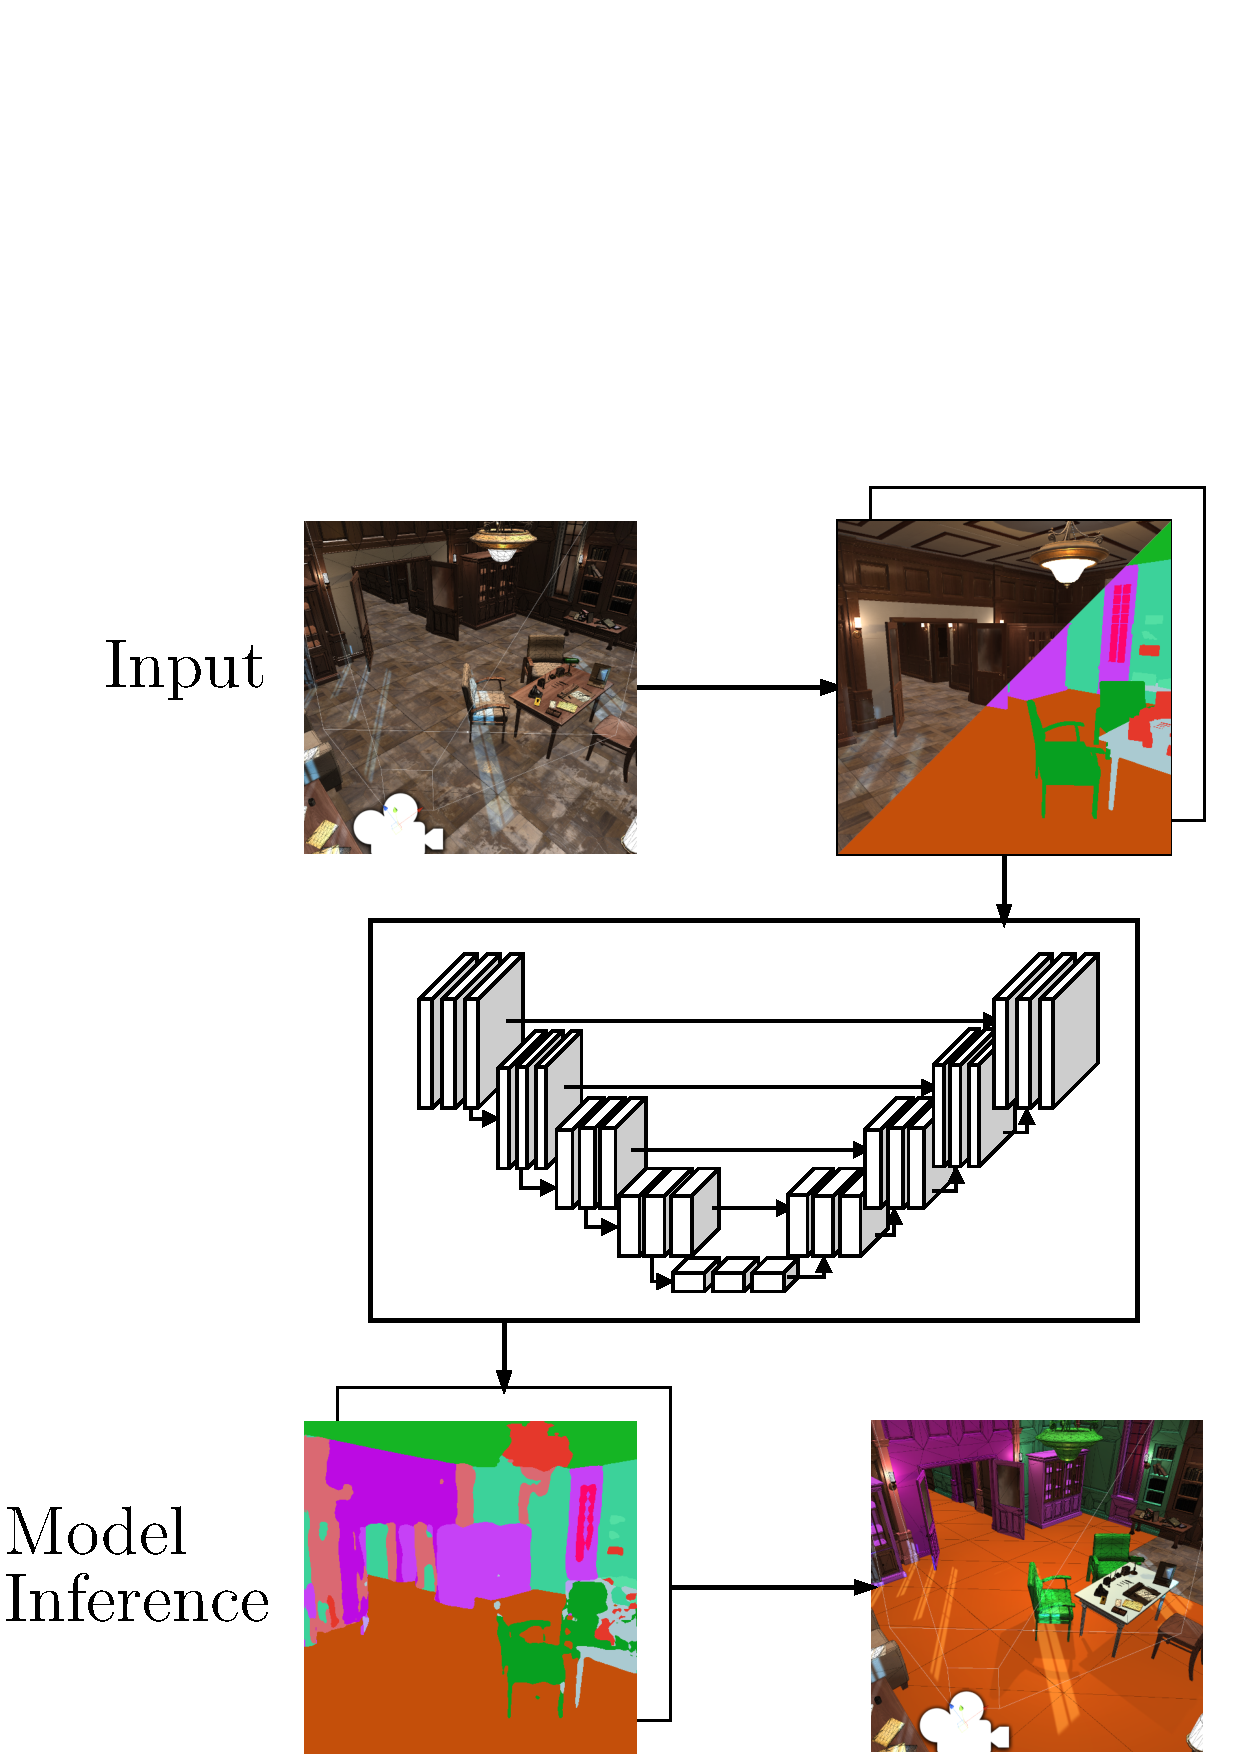
\includegraphics[width=1\linewidth]{camera-pipeline}
    \caption{Overview of the proposed system: given a set of views captured in a VE, a convolutional neural network trained on samples from our scenes performs semantic segmentation. The predicted semantic maps are then reprojected onto objects in the virtual scene, associating predicted semantic classes with acoustic profiles that are attributed to the scene geometry. Tagged scene geometry provides input to acoustic renderers or physically-based audio engines for sound propagation or synthesis tasks.}
    \label{fig:cog-pipeline}
\end{figure}

\paragraph{Training Phase}
The training phase used an environment with scene geometry tagged with ground truth acoustic materials, reproducing the workflow of audio engineers authoring virtual complex scenes by assigning acoustic properties to scene elements. The system is trained on these scenes by generating a set of camera renders with associated segmentation mapping to the correct pixel-wise category.
\begin{figure}[htbp]
    \centering
    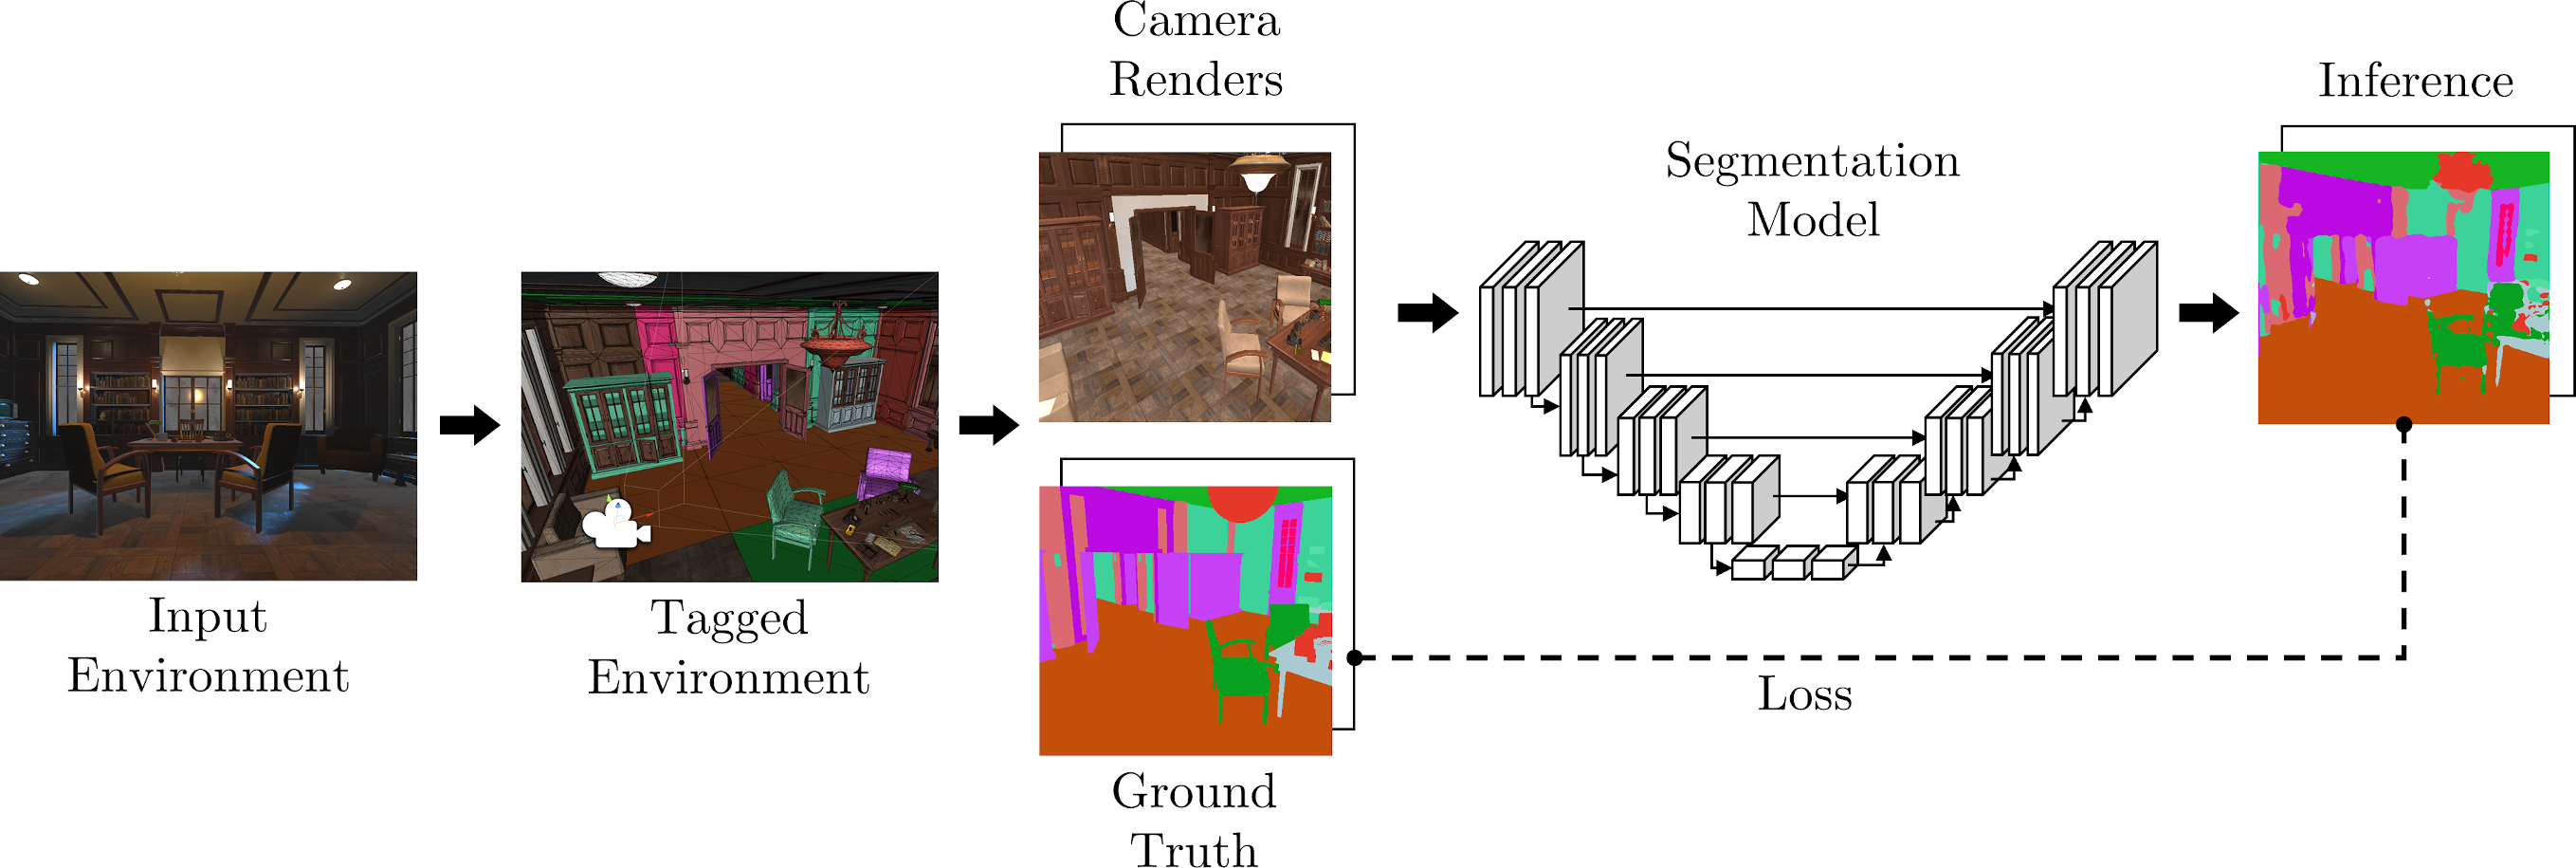
\includegraphics[width=1\linewidth]{cog-pipeline-training}
    \caption{Training phase of the system pipeline: manual acoustic material tagging is performed on an input environment, generating pairs of camera renders and segmentation maps via ray casting, which are then used to train and evaluate the convolutional neural network.}
    \label{fig:cog-training}
\end{figure}

\paragraph{Inference Phase}
Once the network is fit on the ground truth set, it is deployed to a set of test scenes with no material tags, obtaining camera renders across uniformly spaced camera probes scattered around the walkable space of each scene. The scene is then tagged by predicting segmentation maps and reprojecting acoustic material to virtual geometry.
\begin{figure}[htbp]
    \centering
    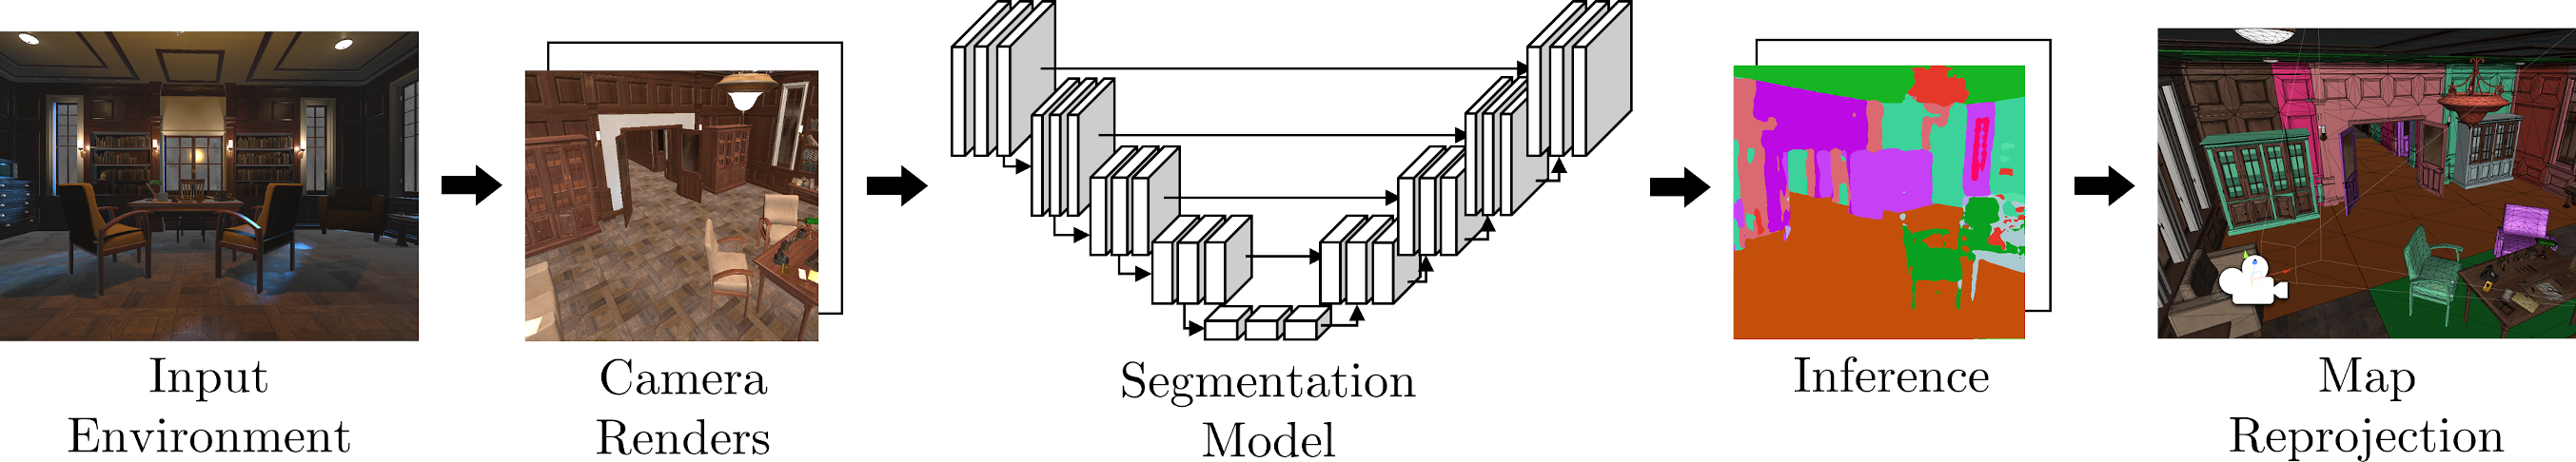
\includegraphics[width=1\linewidth]{cog-pipeline-inference}
    \caption{Inference phase of the system pipeline: camera renders are generated from an input environment, providing input to the convolutional neural network. With camera transformations, segmentation maps generated by the network are used to attribute acoustic properties via semantic class mapping to scene geometry.}
    \label{fig:cog-inference}
\end{figure}



\subsection{Method}
\label{sec:mat-method}
Based on advances in scene understanding and the current state of wave-based audio renderers, we design an architecture that enables the process of semantic mesh labelling in complex scenes and associating every category with a frequency-dependent acoustic absorption function. Methods based on perceptual metrics should consider only meshes that are relevant to the acoustic environment. Scene understanding methods and inference should be optimised depending on the scene geometry.

\subsubsection{Input}
We demonstrate the usage of the pipeline in two scenes: an open, urban environment, \emph{City}, and an indoor wooden room, \emph{Office}. City has $6.3M$ triangles and $8.6M$ vertices. Office has $3.3M$ triangles and $3.8M$ vertices. 
We define a set of classes using tables of measured acoustic absorption of construction materials, where materials are grouped in categories specifying a vector $\alpha$ of absorption coefficient values across an approximated equivalent rectangular bandwidth frequency scale ranging from $125Hz$ to $4kHz$. For every major material category that exists in our material database, we define two levels, representing the low and high bounds of mass density $\rho$ in that category. Mass density is a physical property allowing for the acoustic properties of two objects made of the same material to be perceptually distinguishable \cite{giordano2006material}. 
We define 23 material classes constituted by the two density levels for each of the 11 material categories and an additional class representing ``air'', see Table.

\subsubsection{Data Generation}
We implement the core material tagging system in Unity using a camera located across probe points of a complex scene. Segmentation masks associated with each view are generated by ray-casting through each point of $C_n$, the \emph{near} camera clipping plane, to $\infty$. For this case, we exclude wavelength-based strides to maximise segmentation accuracy. The areas where rays intersect with $C_f$, the \emph{far} camera clipping plane, are labelled as air; objects that are hit by a ray determine the pixel value of the mask, which points to the corresponding material. The dataset consists of 3500 labelled images with $512\times512$ pixel resolution, split into 3000 training images and 500 validation images. 
In City and Office, rendered views are generated in different regions of the environments. The different regions delimit spaces for the collection of training and validation data. For each delimited region, sets of points are scattered to cover the walkable space. The camera position is interpolated across points in these sets and rotated between 0 and $2\pi$ along the azimuth and between 0 and $\pi$ along the elevation.

\subsubsection{Semantic Segmentation Model}
A convolutional neural network is used to discriminate materials of objects represented in the camera-rendered views. This task is performed with pixel-level semantic segmentation using a ResNet-34-based UNet \cite{ronneberger2015u}. The ResNet backbone offers a topology that is easy to train and has excellent generalisation performance. It also provides a compromise between accuracy and the number of parameters \cite{he2016deep}.
The model, pre-trained on the ImageNet dataset, is fine-tuned for 70 epochs minimising focal loss \cite{lin2017focal}. Table \ref{table:model} shows the information on the networks trained, including the total number of parameters, $F_{1}$\hyp{}score, intersection-over-union (IOU) and the number of epochs.
\begin{table}[htbp]
\caption{CNNs used to produce segmentation maps with the camera-based system, detailing architecture type and performance metrics.}
\centering
\begin{tabular}{lllllll}
\toprule
\textbf{Architecture} & \textbf{Backbone}  & \textbf{Capacity} & \textbf{$\mathbf{F_{1}}$\hyp{}score}   & \textbf{IOU}  & \textbf{Epochs} & \textbf{Loss} \\
\midrule
Unet                  & ResNet-34          & $24.5M$           & $0.51$                                 & $0.58$         & $70$           & $2*10^{-3}$   \\
Unet                  & ResNet-50          & $32.6M$           & $0.54$                                 & $0.47$         & $70$           & $7*10^{-4}$   \\
\bottomrule
\end{tabular}
\label{tab:cog-model}
\end{table}

\subsubsection{Model Inference}
The output of the model is an $m \times n \times k$ matrix $M$, where $m$ and $n$ are the input image resolution and $k$ is the number of classes. For each pixel, the $k$ channels encode a probability distribution across the classes. Per-pixel classes are determined with the member having the highest presence probability, reducing $M$ to an $m \times n$ matrix where entries encode the semantic class (see Table \ref{tab:absorption-coeffs}). 
In addition, counts of unique entries in $M$ determine the number of pixels describing the associated material. With scaling based on the distance between a target object and $C_n$, this allows material exclusion below a threshold.

\subsubsection{Map Reprojection}
Using the segmented images, meshes are labelled by raycasting through $C_n$ divided in strides. Based on the distance of every Mesh Renderer Unity object inside the camera frustum, the stride size is determined by the lowest structural dimension of each mesh, scaled according to its distance to $C_n$. This allows consideration of filtering objects by wavelength, $\lambda = 0.7m$, from the reprojection process. This is because some objects are too small to have a significant impact on the human perception of the soundscape \cite{pelzer2010frequency}. Through this level of detail (LOD) graduation, we reduce the analysed scene geometry, excluding structures having smaller perceptual impacts on the resulting acoustic model. Among the factors affecting the performance and accuracy of acoustical simulation methods is the polygon count of the acoustic VE, dependent on the complexity of a scene and the presence of detail and small objects. 
In acoustic environments, smaller structures on surfaces tend to induce scattering of incidental high-frequency waves reflected, and they are neglected by lower frequencies whose wavelength is greater than the structure dimensions. As a consequence, the amplitude of lower frequencies is more likely to be affected by first-order room modes, given by walls and large boundaries, affecting the frequency response of the sound field resulting in a more noticeable perceptual effect. As opposed to frequencies higher than the Schroeder Frequency, which tend to scatter chaotically \cite{kuttruff2016room, blauert1997spatial}.
A pilot study of this perceptual optimisation demonstrates up to 123\% of performance gains in offline and real-time acoustic modelling implementations. Small structures on surfaces can therefore be excluded from modelling processes. Results of this process can be seen in Fig. \ref{fig:results} where smaller objects than this $\lambda$ of 0.7m do not receive a material tag. Considering meshes inside the camera frustum, marching cubes algorithms should enable the geometry reduction considering the size of cubes dependent on the wavelength of the lowest frequency \cite{pelzer2010frequency}.
\begin{figure}
    \centering
    \begin{subfigure}[t]{0.49\textwidth}
       \centering
       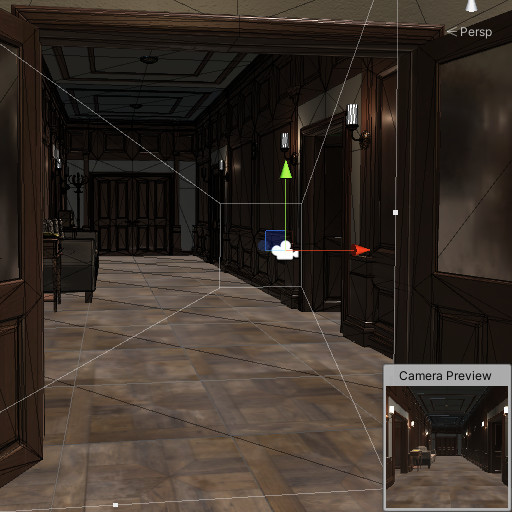
\includegraphics[width=\textwidth]{cog-reproj-a}
       \caption{Input Camera Render}
       \label{fig:cog-reproj-a}
    \end{subfigure}
    \begin{subfigure}[t]{0.49\textwidth}
       \centering
       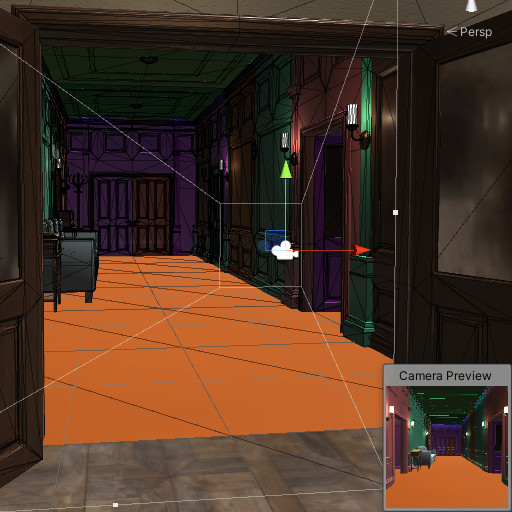
\includegraphics[width=\textwidth]{cog-reproj-b}
       \caption{Re-projected Acoustic Materials}
       \label{fig:cog-reproj-b}
    \end{subfigure}
\caption{Map Reprojection performed on an input camera render: based on a predicted segmentation map, acoustic materials determined by pixel-wise semantic information is re-projected onto scene objects captured by the camera.}
\label{fig:cog-reprojection}
\end{figure}

CASE WHERE MULTIPLE PIXELS PROJECT ONTO THE SAME OBJECT

\subsection{Acoustic Materials}

\begin{table}
    \def\widthspark{120pt}
    \centering
    \caption[Acoustic material definitions]{Common acoustic absorption coefficients with ranges (low-high) of $\alpha$ absorption characteristics across the frequency bands for those material types. It should be noted that these are regressions and averages of generally adopted materials and existing measurement tables; realistic or surveying acoustic simulations should adopt absorption measurements of real materials.}
    \begin{tabular}{lll}
    \toprule
    \textbf{Material}                  & \textbf{Low $\alpha$}                                                              & \textbf{High $\alpha$}                                                               \\ \midrule
    Glass and glazing                  & 
\includegraphics[width=\widthspark]{sparklines/glass and glazing_low}               & 
\includegraphics[width=\widthspark]{sparklines/glass and glazing_high}               \\ 
    Masonry walls                      & 
\includegraphics[width=\widthspark]{sparklines/masonry walls_low}                   & 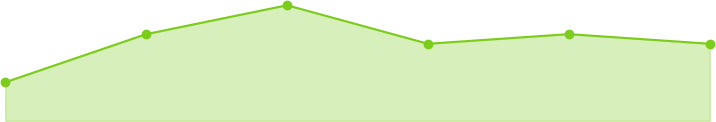
\includegraphics[width=\widthspark]{sparklines/masonry walls_high}                   \\ 
    Stud-work \& lightweight walls     & 
\includegraphics[width=\widthspark]{sparklines/studwork and lightweight walls_low}  & 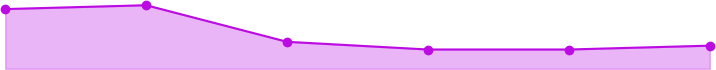
\includegraphics[width=\widthspark]{sparklines/studwork and lightweight walls_high}  \\ 
    Wood \& wood panelling             & 
\includegraphics[width=\widthspark]{sparklines/wood and wood panelling_low}         & 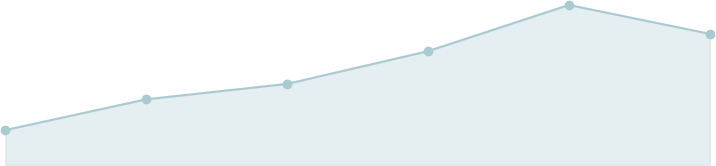
\includegraphics[width=\widthspark]{sparklines/wood and wood panelling_high}         \\ 
    Floors                             & 
\includegraphics[width=\widthspark]{sparklines/floors_low}                          & 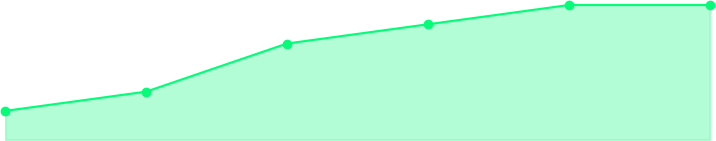
\includegraphics[width=\widthspark]{sparklines/floors_high}                          \\ 
    Panels \& doors                    & 
\includegraphics[width=\widthspark]{sparklines/panels and doors_low}                & 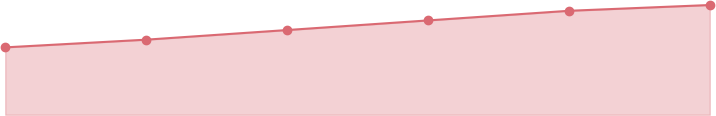
\includegraphics[width=\widthspark]{sparklines/panels and doors_high}                \\ 
    Other                              & 
\includegraphics[width=\widthspark]{sparklines/other_low}                           & 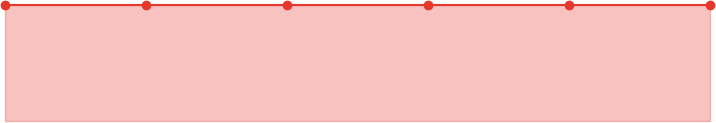
\includegraphics[width=\widthspark]{sparklines/other_high}                           \\ 
    Wall treatments \& construction    & 
\includegraphics[width=\widthspark]{sparklines/wall treatments & constructions_low} & 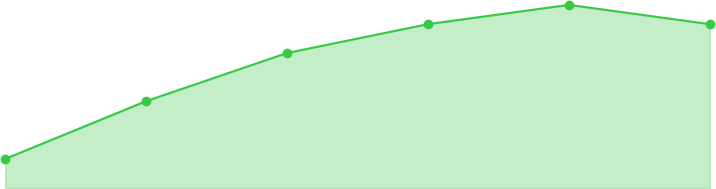
\includegraphics[width=\widthspark]{sparklines/wall treatments & constructions_high} \\ 
    Ceilings                           & 
\includegraphics[width=\widthspark]{sparklines/ceilings_low}                        & 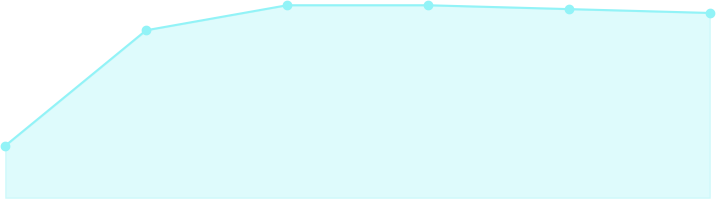
\includegraphics[width=\widthspark]{sparklines/ceilings_high}                        \\ 
    Mineral wool \& foams              & 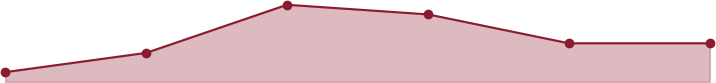
\includegraphics[width=\widthspark]{sparklines/mineral wool and foams_low}          & 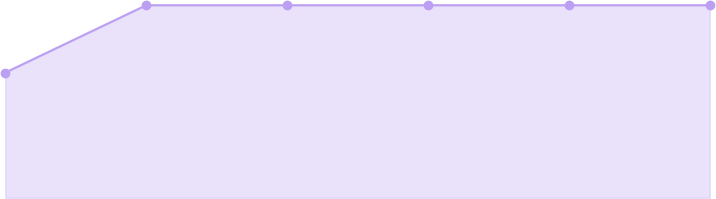
\includegraphics[width=\widthspark]{sparklines/mineral wool and foams_high}          \\ 
    Audience \& seating                & 
\includegraphics[width=\widthspark]{sparklines/audience and seating_low}            & 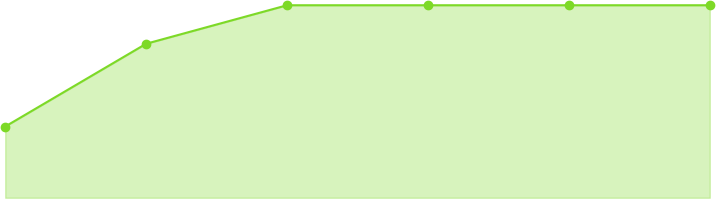
\includegraphics[width=\widthspark]{sparklines/audience and seating_high}            \\ 
    \bottomrule
    \end{tabular}\label{tab:absorption-coeffs}
\end{table}

\subsubsection{Preliminary Evaluation}
An acoustic renderer is used to test the validity of this method by producing auralisations of Office. City is excluded because of its computationally-expensive scene complexity. We employ a state-of-the-art acoustic renderer \cite{raghuvanshi2014parametric}, integrated into Unity, to generate a model of the acoustic environment in which all meshes having a potential impact on the VE are included. The renderer determines per-mesh absorption information based on the texture meta-data as per Default behaviour. A sound source and listener are placed at human height in the scene; the listener captures a $30s$ chirp signal sweeping logarithmically from $20Hz$ to $20kHz$ emitted by the sound source to measure an IR. Maintaining the same settings and positions of source and listener, we repeat the procedure supplying meshes and absorption information inferred by our system, Tagged. We compare the two IRs generated by the former (Default) and the latter acoustic model (Tagged) through comparisons of their deconvolved frequency responses, see Fig.

\subsection{Results}
The model inference takes an average of $400 ms$ and the re-projection process takes an average of $96ms$. These figures are quoted per camera probe that is used to generate acoustic labels for surfaces in the scene. Images to be inferred are of a fixed size from the scene frame buffer, $512 \times 512$ pixels. The time taken for inference is largely invariant to typical scene complexities such as shape, polygon count, materials etc. The Office scene requires 12 probes to completely tag the environment, requiring $\sim$6s to complete the tagging process. The City scene shown, has extra complexity and requires use of solutions to the Art Gallery problem to deduce the minimum number of probes to cover the space and tag all objects. 
As shown in Fig. \ref{fig:results}, acoustic properties can be associated with geometry in the scene, and can be tagged from camera probes. These materials are used in an acoustic rendering process, either directly in game audio engines or external offline acoustic renderers. This can result in more realistic aural spatialisation, using IRs to encode early and late reflections. An example of this offline rendering is shown in Fig. \ref{fig:fft}. 
Currently our approach works by providing inference for camera views within the scene. These camera views are manually placed and would need to be placed in many positions in order to tag materials accurately for the entire scene. This process still requires a human-in-the-loop and needs to be addressed to ensure the goal of having this system as an end-to-end autonomous vision based material tagging system. 
To extrapolate materials tagged to the entire scene, solutions to the Art Gallery problem would optimise the number of predictions required \cite{devadoss2011discrete, bajuelos2008optimizing}. Considering the polygons encapsulating the walkable space $W$ of a scene, minimum vertex guard algorithms suggest that $\floor*{n/3}$, where $n$ indicates the total vertices of $W$, is the least number of positions from where the entire scene can be seen. Based on the depth of the camera, additional intermediate positions $\textbf{p}$ might be needed to accurately represent objects, this also depends on the number of pixels per object allowing the the neural network to infer materials from the set of camera views that facilitate the whole scene to be visible. For each camera probe position, rotation steps are needed to ensure that all points of $W$ are inside the camera frustum. For an omni-directional camera probe, these rotation steps $\textbf{r}_\theta$ for azimuthal steps and $\textbf{r}_\phi$ for elevation steps should cover the space in $2\pi$ azimuth and $\pi$ elevation. The resulting complexity of the material tagging process for the scene would then be determined by $O(\floor*{n/3} + \textbf{p} + \textbf{r}_\theta + \textbf{r}_\phi)$.

\begin{landscape}
\begin{table}[]
\def\cogimsw{0.19\textwidth}
\centering
\caption{Results from tests conducted on the City and Office complex scenes by applied the camera-based acoustic material tagging system.}
\begin{tabular}{@{}lllllll@{}}
\toprule
Render & Input & Segmented & Tagged & Render & Input & Segmented \\ \midrule
\multicolumn{1}{c}{}  & \multicolumn{3}{c}{Office} & \multicolumn{3}{c}{City} \\
\multicolumn{1}{c}{A} &  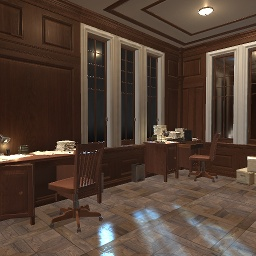
\includegraphics[width=\cogimsw]{Office_A_original} & 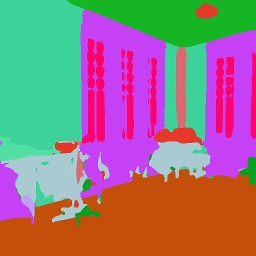
\includegraphics[width=\cogimsw]{Office_A_segmented} & 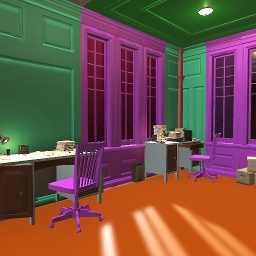
\includegraphics[width=\cogimsw]{Office_A_tagged} & 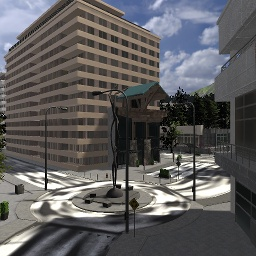
\includegraphics[width=\cogimsw]{City_A_original} & 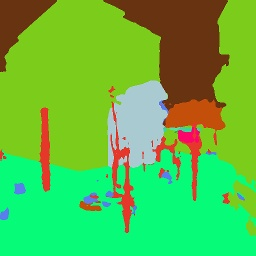
\includegraphics[width=\cogimsw]{City_A_segmented} & \includegraphics[width=\cogimsw]{City_A_tagged} \\
B & \includegraphics[width=\cogimsw]{Office_B_original} & \includegraphics[width=\cogimsw]{Office_B_segmented} & \includegraphics[width=\cogimsw]{Office_B_tagged} & \includegraphics[width=\cogimsw]{City_B_original} & \includegraphics[width=\cogimsw]{City_B_segmented} & \includegraphics[width=\cogimsw]{City_B_tagged} \\
C & \includegraphics[width=\cogimsw]{Office_C_original} & \includegraphics[width=\cogimsw]{Office_C_segmented} & \includegraphics[width=\cogimsw]{Office_C_tagged} & \includegraphics[width=\cogimsw]{City_C_original} & \includegraphics[width=\cogimsw]{City_C_segmented} & \includegraphics[width=\cogimsw]{City_C_tagged} \\
D & \includegraphics[width=\cogimsw]{Office_D_original} & \includegraphics[width=\cogimsw]{Office_D_segmented} & \includegraphics[width=\cogimsw]{Office_D_tagged} & \includegraphics[width=\cogimsw]{City_D_original} & \includegraphics[width=\cogimsw]{City_D_segmented} & \includegraphics[width=\cogimsw]{City_D_tagged} \\
\multicolumn{1}{l}{legend} & \multicolumn{6}{c}{legend}
\end{tabular}
\label{tab:cog-preliminary-results}
\end{table}
\end{landscape}


\subsection{Discussion}
Acoustic modelling and audio rendering methods can benefit from research and development of computer vision methods. 
The current status of this work does not eliminate the human-in-the-loop; however, it can generalise and operate on large sets of complex scenes. As a result, artistic and creative workflows for level design can benefit from automated material tagging system that is agnostic of scene complexity and allow for easy integration of wave-based acoustic renderers.
The next steps planned for this work include the development of a generalised system to perform material tagging in complex scenes. This will consider optimisation methods to allow the inference of entire scenes automatically with the minimal set of camera probes to consistently tag every acoustically congruent object that is contributory to the VE.\par
One crucial advantage of a camera-based acoustic material recognition system is the potential to tailor the recognition of materials based on their appearance to a defined ecosystem of material appearances expressed by a set of virtual environments. Although this aspect contrasts the goal of CNN of providing generalisable models, it addresses the problem of the large variance found in visual features of materials by constraining the network within a range of material appearances that interest VE designers. Resembling workflows common in Neural Radiance Fields \citep{mildenhall2020nerf}, game designers or VE artists would need to provide exemplary scenes tagged with a customisable set of acoustic and semantic materials to the camera-based system, enabling acoustic material tagging of unseen or novel scenes sharing the same nature. With the rising availability of computational resources allocated to rendering VEs, performing a forward pass with a ResNet50 CNN \citep{he2016deep} is becoming feasible at runtime, unlocking the potential for online sound propagation on dynamic scenes.\par

% Case for tailoring material recognition to ecosystems of materials
Case for artistic material tags


\section{Texture-based Acoustic Material Tagging}\label{sec:texture-tagging}
Here, we propose a novel architecture for tagging acoustic material in virtual environments, which improves upon recent work by abstracting away from camera-based systems and tests vision-based material recognition methods in real environments. By working on virtual reconstructions of complex scenes, the approach is agnostic of the technology and architecture of the target platform. Despite the significant progress made in sound propagation over the last decades, there are still many limitations in simulations for indoor and outdoor environments due to the complexity of the factors that describe a wavefield \cite{liu2020sound}. This improved system expands from the camera-based methods by contributing towards:
\begin{itemize}
    \item a more efficient application of acoustic rendering to virtual environments;
    \item a novel architecture for recognising materials from textured meshes in complex scenes, reducing the need for manual tagging of acoustic materials and eliminating the needs for camera-based workflows; 
    \item an objective evaluation of the architecture conducted on a virtual reconstruction of a real conference room.
\end{itemize}

\subsection{Method}
We present a method for processing scene geometry generating acoustic models by predicting materials of objects composing complex scenes. A breakdown of the system shown in Figure~\ref{fig:pipeline_overview} illustrates how visual representations of the environment map to acoustic data used by sound renderers to model sound propagation in a scene. The unwrapped texture of each mesh in the scene geometry provides representations of their materials, which provide input for a convolutional neural network. The network, based on features extracted from textures, recognises different material labels in textures and maps them to acoustic data from a database, expressed as acoustic materials.

\subsubsection{Material Recognition}
According to \cite{schwartz2019recognizing}, small image patches contain enough information to distinguish materials and hence, we decompose input image textures into small image patches.
\subsubsection{Training}
\begin{figure}[htbp]
    \centering
    \includegraphics[width=1\linewidth]{chi-training}
    \caption{}
    \label{fig:chi-inference}
\end{figure}
We determine the visual material space by applying transfer learning to the OpenSurfaces dataset \cite{bell2013opensurfaces}, which comprises 36 classes of surface photographs. 
The SLIC algorithm \cite{slic6205760} segments input surface photographs into a set of superpixel labels, which determine regions correlated with boundaries of objects. From these resulting superpixel labels, we then generate rectified image patches encapsulating their contours through edge detection \cite{ding2001canny}.
The rectified image patches are fed through a ResNet50 \cite{he2016deep}, used as a feature extractor for a classification network using a standard fully connected layer to predict class labels based on embeddings of 32x32 pixel resolution input patches. We train the network on 13677819 input patches, composing a train set of about 9.1M images and an evaluation set of about 4.5M, adopting the standard Adam optimiser \cite{kingma2014adam} to update the weights initialised from the ImageNet dataset \cite{deng2009imagenet}. The model usually converges in 45 epochs with a training and validation accuracy of about 0.94 and 0.83 respectively. 

\subsubsection{Inference}
\begin{figure}[htbp]
    \centering
    \includegraphics[width=1\linewidth]{chi-inference}
    \caption{}
    \label{fig:chi-inference}
\end{figure}
Given the set of textured meshes in a scene, we unwrap textures as images to predict materials represented. The trained ResNet50 extracts features from input image textures in complex scenes, whose embeddings enable the classifier to predict class labels associated with each input superpixels. The most frequent prediction maps to an acoustic measurement database, defining the output acoustic material. On average, the classifier takes $11.2s$ to determine the acoustic material for a given texture, see Figure~\ref{fig:superpixel_labels}, divided in $3.8s$ for generating rectified patches and $7.3s$ to extract features and compute the mapping.%

\subsubsection{Acoustic Material Mapping}
Material labels inferred from textures are associated with acoustic measurements of absorption coefficients. For every label, a one-to-many mapping groups measurements of the given material. Following the methodology in \cite{kim2020acoustic}, we use median frequency-dependent values to determine acoustic absorption, defining acoustic materials. A single acoustic material maps to each given mesh, associating a vector of acoustic absorption coefficients to its triangles, determining the overall acoustic mapping accuracy to depend upon the mesh separation of the scene geometry. In the example texture shown in Figure~\ref{fig:superpixel_labels}, ``Tile'' defines the acoustic material, as per predictions shown in Figure~\ref{fig:hist}.
\begin{figure}
    \centering
    \begin{subfigure}[t]{0.49\textwidth}
       \centering
       \includegraphics[width=\textwidth]{slic-input-texture}
       \caption{Input Texture}
       \label{fig:slic-input-texture}
    \end{subfigure}
    \begin{subfigure}[t]{0.49\textwidth}
       \centering
       \includegraphics[width=\textwidth]{slic-texture}
       \caption{SLIC Superpixels}
       \label{fig:slic-labels}
    \end{subfigure}
\caption{SLIC Superpixel computation on real texture from a scanned space.}
\label{fig:slic-generation}
\end{figure}

\begin{figure}[htbp]
    \centering
    \includegraphics[width=1\linewidth]{slic_labels}
    \caption{Predicted Class labels from input image patches computed from the texture shown in Figure~\ref{fig:slic-generation}.}
    \label{fig:slic-labels}
\end{figure}



\subsection{Preliminary Evaluation}
We compare acoustic models estimated with state-of-the-art wave-based audio renderers, testing whether the proposed system for the automatic tagging of scene geometry has a significant impact on the resulting acoustic model. The experimental evaluation uses a real environment as a benchmark for testing how predicted models express acoustic parameters of measurable space.

\subsubsection{Scene Geometry Reconstruction}
Wavefields are simulated from a real conference room that is $3.5346m$ deep, $2.8367m$ wide and $3.5149m$ tall. Theoretically, the dimensions determine a Schroeder frequency of $261Hz$. The room is reconstructed using the Unity game engine with $2.9M$ of triangles and $6.6M$ vertices.
We reconstruct the geometry of a conference room to deploy the proposed system in a real environment and conduct the subsequent subjective experimental evaluation. We adopt a LiDAR scanner, FARO Focus\textsuperscript{3D} X300, to capture several point clouds scans of the room across 8 positions: 4 position points for each corner of the room at about 1$m$ height and 4 additional positions at about 0.2$m$ height to capture furniture and materials from different angles and enhance the spatial resolution. We then segment the reconstructed mesh, obtained from the scanner, to ensure that every scene object is represented by a separate textured mesh.
\begin{figure}
    \centering
    \begin{subfigure}[t]{0.49\textwidth}
       \centering
       \includegraphics[width=\textwidth]{environment}
       \caption{Input Camera Render}
       \label{fig:chi-input-env}
    \end{subfigure}
    \begin{subfigure}[t]{0.49\textwidth}
       \centering
       \includegraphics[width=\textwidth]{reconstructed}
       \caption{Re-projected Acoustic Materials}
       \label{fig:chi-reconstructed-env}
    \end{subfigure}
\caption{Map Reprojection performed on an input camera render: based on a predicted segmentation map, acoustic materials determined by pixel-wise semantic information is re-projected onto scene objects captured by the camera.}
\label{fig:chi-scanning}
\end{figure}


\subsubsection{RIR Measurements}
The experimental evaluation compares simulated wavefields generated from the reconstructed environment to a sample measurement of the real counterpart's wavefield. We compare wavefields using Room Impulse Responses (RIRs) to describe acoustic properties dependent on geometry and materials surrounding a sound transmission between a source and a listener \cite{stan2002comparison}. We capture the environments' acoustic characteristics emitting and recording an exponentially swept sine, ranging from $20Hz$ to $20kHz$, from a listening to a receiving point that is consistent between the real and reconstructed environments, see Figure~\ref{fig:pipeline_overview}. Applying inverse filtering, we recover the RIRs from the captured signal \cite{holters2009impulse}. Given the single listener position, all RIRs are mono.
% \subsubsection{Real environment}
In the conference room, a public address system, the dB Technologies ES 1002, emitted the exponentially swept sine converted from a laptop using an Audient ID14 DAC and ADC, which captured the signal back through an omnidirectional measurement microphone, the Earthwork M30.
% \subsubsection{Reconstructed Environment}
With Steam Audio \cite{audio2019git}, we simulate wavefields of the reconstructed environment.  This allows synthesis of wavefields based on acoustic geometry, considering absorption coefficients expressed across three frequency bands: low, medium and high. All simulations share the same resolution of 65536 and 16384 direct and secondary rays, respectively, with 256 bounces off solid geometry. With the same setup, we synthesise three wavefields with different acoustic materials: the \emph{generic} with a single acoustic material for the entire scene geometry; the \emph{tagged}, with acoustic materials assigned through manual material tagging; and \emph{ours}, using the proposed automatic tagging.
\subsubsection{Perceptual test}
We conduct a perceptual comparison between simulated wavefields at the same positions of source and listener, see Figure~\ref{fig:reconstruction}, using an automated perceptual metric learned on subjects’ responses \cite{manocha2020differentiable}. The metric consists of a 14-layer deep neural network with filters trained on features extracted from paired input audio samples; it expresses a distance $D(x_{ref}, x_{per})$ between two input signals, where $x_{ref}$ is a reference signal, and $x_{per}$ is a perturbated signal. The function $D$ considers factors including reverb and the ratio between direct and reverberated signal. We test whether the metric expresses a closer perceptual distance between the measured ground truth and the synthesised wavefields, by convolving the RIRs to samples from the evaluation subset of a database for acoustic scene classification, which comprises 15 different acoustic environments, generating a total of 18 minutes of audio over 1620 $N$ samples \cite{mesaros2016tut}. The learned metric determines the distance between the ground truth convolutions and each of the relative simulated RIRs: for each audio sample $k$ in $N$, we determine perceptual distances $D(x_{ref, k}, x_{per_i, k}~\forall~i \in \{generic, tagged, ours\})$, where $ref$ and $per_i$ are the measured and simulated RIRs.

\subsection{Evaluation Results}
figures.

\section{Proof of Concept Demonstration}
An experimental evaluation is designed to investigate the performance of the proposed material tagging prototypes in attributing acoustic properties to segments of the scene geometry of a given environment expressed as a set of triangulated meshes. The evaluation focuses on scenes scanned with space reconstruction techniques applied to real environments, emulating space reconstruction paradigms often adopted by AR HMDs. \par
The evaluation uses standard space-sensing cameras to produce triangulated meshes from a set of real environments. These virtual reconstructions are then processed, segmenting the scene of each environment by generating portions of scene geometry into a set of semantically meaningful sub-meshes expressing elements of the scene. Submeshes are tagged with acoustic material by assigning each scene element, referred to by its sub-mesh, a semantic acoustic material drawn from a generated list of materials defined by each of the two prototypes. \par
The two prototype systems are deployed on the virtual reconstructions of the real spaces, inferring acoustic materials across all scene elements. The evaluation measures the accuracy in assigning the correct semantic information to each scene element, comparing predictions to ground truth acoustic material tags.

\subsection{Test Scenes}
The test adopts three real spaces: a small, a medium, and a large environment, see Table~\ref{tab:material-eval-scene}. These environments have diverse ecosystems of surfaces and materials that characterise and determine their respective soundscape and acoustic fingerprints.
\begin{table}[]
\centering
\begin{tabular}{@{}llllll@{}}
\toprule
Scene               & Dimensions & Volume & Triangles & $T_{60}$ & Segments \\ \midrule
Mastering Suite     & ph         & ph     & ph        & $0.00$   & $00$ \\
Recital Hall        & ph         & ph     & ph        & $0.00$   & $00$ \\
St Mary's Guildhall & ph         & ph     & ph        & $0.00$   & $00$ \\ \bottomrule
\end{tabular}
\caption{Summary of the scenes used for the testing procedure of the acoustic material tagging prototypes.}
\label{tab:material-eval-scenes}
\end{table} %tab:material-eval-scene

\begin{figure}[htbp]
    \centering
    \includegraphics[width=0.7\linewidth]{guildhall}
    \caption{St Mary's Guildhall: a Medieval-style church in Coventry, West Midlands, England. The large environment has a unique soundscape, characterised by a recorded $T_{60}$ reverberation time of over a second.}
    \label{fig:guildhall-iso-render}
\end{figure}

\begin{figure}[htbp]
    \centering
    \includegraphics[width=0.7\linewidth]{recital-hall}
    \caption{Recital Hall: a wooden space serving as a stage for musical performances. The soundscape is characterised by a recorded $T_{60}$ reverberation time within a second.}
    \label{fig:conservatoire-iso-render}
\end{figure}

\begin{figure}[htbp]
    \centering
    \includegraphics[width=0.7\linewidth]{mastering_suite}
    \caption{Mastering Suite: a small audio production studio with acoustic treatments to minimise the effect of the soundscape on the sound reproduction system within.}
    \label{fig:conservatoire-iso-render}
\end{figure}


\begin{figure}
    \centering
    \begin{subfigure}[t]{0.49\textwidth}
       \centering
       \includegraphics[width=\textwidth]{environment}
       \caption{Input Camera Render}
       \label{fig:chi-input-env}
    \end{subfigure}
    \begin{subfigure}[t]{0.49\textwidth}
       \centering
       \includegraphics[width=\textwidth]{reconstructed}
       \caption{Re-projected Acoustic Materials}
       \label{fig:chi-reconstructed-env}
    \end{subfigure}
\caption{Map Reprojection performed on an input camera render: based on a predicted segmentation map, acoustic materials determined by pixel-wise semantic information is re-projected onto scene objects captured by the camera.}
\label{fig:chi-scanning}
\end{figure}


% \begin{figure}[htp]
% \centering 
% \subfloat[St Mary's Guildhall: a Medieval-style church in Coventry, West Midlands, England. The large environment has a unique soundscape, characterised by a recorded $T_{60}$ reverberation time of over a second. ]{%
%   \includegraphics[clip,width=0.5\textwidth]{guildhall}%
% }\\
% \subfloat[Recital Hall: a wooden space serving as a stage for musical performances. The soundscape is characterised by a recorded $T_{60}$ reverberation time within a second.]{%
%   \includegraphics[clip,width=0.5\textwidth]{recital-hall}%
% }\\
% \subfloat[Mastering Suite: a small audio production studio with acoustic treatments to minimise the effect of the soundscape on the sound reproduction system within.]{%
%   \includegraphics[clip,width=0.5\textwidth]{mastering_suite}%
% }\\
% \caption{Environments used for the evaluation of the two prototype systems for acoustic material tagging.}
% \label{fig:material-testing-scenes-iso}
% \end{figure}


\subsection{Mesh Segmentation}
Manual segmentation of scene geometry via Blender.

\subsection{Manual Acoustic Material Tagging}
The segmented meshes are then manually tagged, assigning acoustic absorption coefficients to the triangles of each sub mesh.

UV Mapping of scene geometry to texture segments.

\begin{figure}
    \centering
    \begin{subfigure}{0.75\textwidth}
        \includegraphics[width=\textwidth]{floor0}
        \caption{Scene Geometry: Floor}
        \label{fig:floor}
    \end{subfigure}
    \hfill
    \begin{subfigure}{0.42\textwidth}
        \includegraphics[width=\textwidth, height=\textwidth]{uv_floor0}
        \caption{Texture Mapping 1}
        \label{fig:uv_floor}
    \end{subfigure}
    \hfill
    \begin{subfigure}{0.42\textwidth}
        \includegraphics[width=\textwidth, height=\textwidth]{uv_floor1}
        \caption{Texture Mapping 2}
        \label{fig:uv_floor2}
    \end{subfigure}
            
    \caption{UV mapping of one scene geometry segment to many texture segments.}
    \label{fig:uv_mapping_demo}
\end{figure}


\subsection{Testing methodology}
RIR comparisons across single sources. Manually tagged and automatically tagged should be close perceptually.


\section{Results}
Results from camera and superpixel.



\section{Discussion}
Both systems provide fundamental building blocks for acoustic material tagging for AAR pipelines.

\section{Conclusions}

\subsection{Contributions}
Camera-based system for acoustic material tagging.

\subsection{Future Research Directions}
% Camera-based
Acoustic modelling and audio rendering methods can benefit from research and development of computer vision methods. 
The current status of this work does not eliminate the human-in-the-loop; however, it can generalise and operate on large sets of complex scenes. As a result, artistic and creative workflows for level design can benefit from automated material tagging system that is agnostic of scene complexity and allow for easy integration of wave-based acoustic renderers.
The next steps planned for this work include the development of a generalised system to perform material tagging in complex scenes. This will consider optimisation methods to allow the inference of entire scenes automatically with the minimal set of camera probes to consistently tag every acoustically congruent object that is contributory to the VE. 
% superpixel
We addressed the problem of mapping acoustic absorption data to scene geometry in virtual environments for acoustic simulations. Methods and frameworks for material recognition have become efficient enough in recognising materials in the wild with varying factors of illumination, shape and surface characteristics. Despite their limited resolution in computer games applications, sound propagation systems benefit from acoustic material tagging. With the proposed system, we aim to integrate material recognition to wave-based methods to determine materials' acoustic properties.
The next steps of this work aims to extend the system to broader scenes with larger sets of materials as well as improving the material recognition by performing multi-scale analysis of superpixels and adopting clustering paradigms to overcome the limitations of finite material space definitions.
With the proposed system, we aim to employ these methods to eliminate the human-in-the-loop for the process of labelling materials for acoustic renderers or assist in artistic and creative processes for level design. 


% \chapter{Geometrical Acoustics Rendering Pipelines for Augmented Acoustics}\label{ch:acousticrendering} % If you're changing this, update Section 1.6

This chapter shows the prototyping of a bespoke acoustic rendering pipeline for dynamic virtual environments that integrates material recognition that can extend to immersive technology applications. The design process started with a simplistic form of acoustic rendering, using a standard method to approximate reverb, and expanded towards a bespoke ray tracing-based system that handles dynamic geometry.

\section{Image Source-Based Rendering}
The initial prototype acoustic renderer developed for this research utilises the \acrfull{ism}, a method for simulating reverberation in cuboid environments. This Chapter delves into the principles, implementation, and evaluation of several acoustic renderers, providing insights into their advantages and limitations. The \acrshort{ism} is a simple approach to rendering that approximates reverberation by simulating the reflections of sound waves off the surfaces of a cuboid environment, representing a useful choice for prototyping. By treating each reflection as an image source, the model can efficiently compute the paths that sound waves take from the source to the listener, accounting for multiple reflections. This method is particularly effective in environments with rectangular geometries, where the predictability of reflections simplifies the calculations involved. As discussed in Chapter~\ref{ch:Background}, the \acrshort{ism} technique is well-established in the sound rendering research domain, offering a balance between computational efficiency and auditory realism  \citep{savioja1999creating, allen1979image}. The technique's ability to quickly simulate reverberation makes it an attractive choice for real-time applications, such as \acrshort{ar}, where responsiveness is crucial. By leveraging the predictable nature of reflections in cuboid environments, \acrshort{ism} can generate realistic reverberation effects with relatively low computational overhead.\par
Figure~\ref{fig:image-source-pipeline} shows how the technique has been integrated into a sound rendering pipeline to compute reflection paths in a given virtual scene reconstruction. As a high-level summary, the \emph{geometry reduction} component of this pipeline decomposes the virtual scene into a simpler cuboid volume. Vision-based material recognition techniques are used to understand the acoustic characteristics of surfaces in the input scene; these characteristics are then mapped onto the appropriate surfaces of the acoustic volume representing the given virtual scene. Finally, the \acrshort{ism} is supplied with spatial information on emitters and listeners to produce RIRs from the acoustic volume.\par

\begin{figure}[htb]
    \centering
    \includegraphics[width=1\linewidth]{image-source-renderer}
    \caption[Image-Source Model-based acoustic rendering pipeline]{The Image Source Model (\acrshort{ism}) pipeline showing the four stages of the rendering process (left to right): an input scene is used as input; a geometry reduction process simplifies the complexity of the virtual environment to a cuboid volume; based on portions of the geometry dictated by the cuboid volume, materials of the input environment are determined; materials and simplified geometry provide input to the \acrshort{ism} to produce reverberation responses.}
\label{fig:image-source-pipeline}
\end{figure}

\subsection{Geometry Reduction}
The \emph{geometry reduction}, Figure~\ref{fig:image-source-pipeline}, generates a binary field, sampling from the input geometry at a given number of points. The field shapes the acoustic volume using a marching cubes algorithm, where each cell captures the appearance of surfaces from textures associated with meshes of the input geometry. A cuboid volume encapsulating the reconstructed surface determines the dimensions of the acoustic space simulated with the \acrshort{ism}. Using the vision-based techniques discussed in Chapter~\ref{ch:Materials} to analyse surface appearance, acoustic materials are inferred per image patch, effectively mapping acoustic materials to the surface of the acoustic volume.\par
Input geometry is decomposed into a binary field expressed as $\mathbf{B} = (b_{x,y,z}) \in \{ 0, 1 \}^{P}$, where $P$ is the number of points sampled across the three dimensions. The definition of $\mathbf{B}$ is relevant to the quality of the resulting acoustic simulation and determines the accuracy of the acoustic material recognition, discussed in the following section. Given the set of input meshes from the complex scenes, we define an \acrfull{aabb} encapsulating all vertices of a given scene object, normalising their coordinates to the $[-1, +1]$ range. Values in $\mathbf{B}$ equate to $1$ whenever a cell is within the coordinates of any \acrshort{aabb} defined and to $0$ otherwise. The term \acrshort{aabb} throughout this Chapter, will refer to the collection of all bounding boxes associated with scene objects throughout the rest of this Section. A multi-threaded implementation of the marching cubes algorithm \citep{bourke1994polygonising, lengyel2019foundations} shapes the binary field into a volume, representing the acoustic environment for reflection path computation. In this process, the use of the \acrshort{aabb} to probe the input scene objects introduces error in cases with concave geometry, which negatively correlates to the resolution of $\mathbf{B}$ as collision checks with AABBs increase with the number of cells. A cuboid encapsulating the reconstructed surface from the marching cubes determines the \acrshort{ism} volume for the reflection computation stage.\par

\subsubsection{Isosurface Reconstruction Error}\label{sec:marching-cubes-error}
The marching cubes algorithm is a powerful tool and a crucial step in the pipeline for reconstructing acoustic volumes by sampling complex geometries at various resolution levels. This technique is useful in acoustic rendering, where accurate representation of three-dimensional surfaces is crucial for simulating sound propagation and interaction with the environment.
One of the key strengths is its speed and efficiency, as the algorithm is highly suitable for parallel processing. This parallelisation capability allows for significant improvements in processing times, which is essential for real-time applications in acoustic rendering. By leveraging modern multi-core processors and GPU acceleration, as seen in similar acoustic rendering using parallelisable computer shaders on GPUs \citep{savioja2010use}, the algorithm can handle large scenes efficiently.\par
Despite its efficiency and adaptability, the marching cubes algorithm has inherent limitations that can affect its performance and accuracy in certain scenarios. It may oversimplify complex geometrical features, for instance, leading to a loss of important details that are crucial for accurate acoustic modeling. This can result in a less precise representation of the surface, affecting the fidelity of sound propagation simulations. The discrete nature of the algorithm can introduce artifacts, especially at lower resolution levels. These artifacts can manifest as unwanted distortions, irregularities, or floating pieces of geometry in the reconstructed acoustic volume, which can impact the accuracy of the acoustic rendering. The algorithm may struggle with accurately capturing sharp edges and corners, which are often critical for realistic sound reflections and diffractions. This limitation can lead to a smoothing effect that diminishes the realism of the acoustic model.\par


\begin{figure}[htb]
    \centering 
    \includegraphics[width=1\columnwidth]{ism-patch_generation}
    \caption[ISM Acoustic Rendering --- surface patch generation diagram]{Image patch generation: surfaces intersected by marching cubes are projected onto image patches with a camera by rasterising vertices via orthographic projections of the delimited portion of the surface. The resulting image patch is then fed to a neural network to extract features for semantic classification. Through a one-to-many mapping, semantics attributed to a patch, via embeddings classification, map to acoustic parameters.}
\label{fig:ism-patch_generation}
\end{figure}

\subsection{Camera Projection}
Image patches are generated whenever a marching cube intersects a surface by an entire side, i.e.\ four consecutive corners of each marching cube. An orthographic camera, positioned at the centre of the neighbouring cube, rasterises sub-surfaces delimited by the cube. The camera is positioned on the opposite side of the four intersected corners, facing the surface that is intersected; see Figure~\ref{fig:ism-patch_generation}. 
By using OpenGL rasterisation, surfaces are renderered orthographically from world space, defining the camera clipping space as the volume of the marching cube. Sampling image data from textures, the rasterisation stage produces an image patch representing the projection of the portion of the surface inscribed by a marching cube. Marching cubes intersecting in four consecutive corners ensure that the orthographic camera is perpendicular to the surface.\par

\subsection{Acoustic Material Classifier}
The acoustic renderer leverages material recognition techniques developed throughout Chapter~\ref{ch:Materials}, specifically adopting surface material classifiers within the context of predicting acoustic characteristics of handled scene geometry. This pipeline uses the geometry reduction component illustrated in earlier Sections to obtain a view of entities and surfaces on which material classifiers are applied.
Image patches projected from marching cubes provide input to a neural network, a ResNet50 \citep{he2016deep} backbone that operates as a feature extractor, whose output is forwarded to a densely connected layer. This last layer classifies predicted embeddings into acoustic material categories. The network was trained on the OpenSurfaces dataset \citep{bell2013opensurfaces}, learning mappings between visual appearances of surfaces from 34 material classes and semantic labels, as described in Chapter~\ref{ch:Materials}. The network, pre-trained on ImageNet \citep{deng2009imagenet}, learns on $32\times32$ pixel resolution image patches that are extracted from appearances sampled from OpenSurfaces, assembling a dataset of about 13M images, split into 9M and 4M train and evaluation sets, respectively. Via a one-to-many mapping, 34 categories from the OpenSurfaces dataset map to acoustic materials, and, given 11 acoustic materials, subdividing into two levels of mass density, the visual labels are mapped to 22 acoustic materials.\par

\subsubsection{Classification Accuracy and Precision}
The process of using visual representations of scene geometry to perform acoustic material inference can be prone to error due to the accuracy and precision of the classifier adopted. As discussed in Section~\ref{sec:texture-tagging}, one crucial problem of material tagging is matching the ecosystem of materials represented by the classifier's training data and the target scene geometry to be predicted. State-of-the-art \acrshortpl{cnn} perform around $94\%$ on in-the-wild datasets like OpenSurfaces \citep{he2016deep, bell2013opensurfaces}. Hence, the acoustic rendering pipeline design should account for misclassified scene geometry segments.\par
The subdivision parameter offered by the geometry reduction components can have control over the impact of prediction errors caused by the classifier by offering coarse or fine subdivisions of the environment. With more subdivisions and a fine subdivision of the environment, the classifier can have more views of the scene geometry. Coarse subdivisions allow fewer predictions but increase the impact of misclassifications. Furthermore, misclassifications have varying degrees of impact on the resulting acoustic simulation: a misclassification of a segment of scene geometry that has low absorption as ground truth will have a higher impact on the simulation if tagged with a high-absorption material. Using materials defined in Table~\ref{tab:absorption-coeffs} as an example, the impact of a misclassification varies depending on the distance between the classified material and the ground truth on the spectrum of acoustic absorption.


\subsection{Frequency-Dependent Reverb Approximation}
As discussed in Section~\ref{sec:intro-immersive-acoustics}, the \acrfull{ism} is a foundational technique used in acoustic rendering to simulate reverberation by modeling the reflections of sound waves within an environment. This model approximates how sound interacts with surfaces, creating virtual ``image'' sources that replicate the effect of reflections. While the \acrshort{ism} is computationally efficient and straightforward, it inherently suffers from limitations that affect its accuracy, particularly in approximating low-frequency reverberation. Techniques exist to overcome the limited representation of low-frequency information, such as wave-based acoustic simulations \citep{hamilton2017fdtd} or hybrid techniques, using wave-based but delegating high-frequency approximation to geometrical acoustics \citep{southern2013room}. However, these techniques have considerable computational resource footprints, making it difficult to integrate them into immersive applications.\par
Considering the pipeline at hand, the \acrshort{ism} offers fast and efficient reverb approximations at a trivial computational load, allowing the integration of computer vision techniques. The \acrshort{ism} estimates attenuation functions for a given listener position, with respect to a source in space, drawing from~\cite{habets2006room} implementation to estimate $h$ reverb response functions based on the spatial $[x, y, z]$ coordinates of a sound source, $\mathbf{s}$, a listener, $\mathbf{l}$, at each time step $t$ as 
\begin{equation}\label{eq:ism-base}
    h(\mathbf{l}, \mathbf{s}, t) = \sum_{\mathbf{p} \in \pazocal{P}} \sum_{\mathbf{m} \in \pazocal{M}} \beta_{-x}^{|\mathit{m_x - q}|} \beta_{+x}^{|\mathit{m_x}|} \beta_{-y}^{|\mathit{m_y - j}|} \beta_{+y}^{|\mathit{m_y}|} \beta_{-z}^{|\mathit{m_z - k}|}  \beta_{+z}^{|\mathit{m_z}|} \frac{\delta(t - \tau)}{4\pi \mathit{d}}\textrm{.}
\end{equation}
Here, $\pazocal{M} = \{(m_x, m_y, m_z): -N \leq m_x, m_y, m_z \leq +N\}$ determines the number of points per dimension based on the size of the input acoustic volume and the timestep, dependent on the desired sampling frequency, on the length of the output \acrshort{rir}, and the order of reflections $N$. $\pazocal{P} = \{ (q, j, k): q, j, k \in {0, 1} \}$ determines possible combinations of image sources mirrored in the three dimensions from every boundary in the acoustic volume to consider higher-order reflections, which are computed by $\delta (t - \tau)$, where $\tau = \frac{||\mathbf{R_p} + \mathbf{R_m}||}{c}$ indicates the reflection time delay by dividing the measured distance between mirrored image positions $\mathbf{R_p} + \mathbf{R_m}$ and the listener by the speed of sound $c$, $d$ is the distance term and is calculated as $\sqrt{(\mathbf{R_m}+\mathbf{R_p})}^2$. With combinations in $\pazocal{P}$, image positions are determined by
\begin{align*}
    &\mathbf{R_p} = [ (1 - 2q)\mathbf{s_x} - \mathbf{l_x}, (1 - 2j)\mathbf{s_y} - \mathbf{l_y}, (1 - 2k)\mathbf{s_z} - \mathbf{l_z} ] 
    \quad \textrm{and} \\
    &\mathbf{R_m} = [2 m_x l_x, 2 m_y l_y, 2 m_z l_z]\textrm{.}
\end{align*}
The \acrshort{ism} computes multiple $h$ functions across frequency-dependent reflection coefficients, increasing the accuracy of simulated reflections from boundaries of the acoustic volume. In Equation~\ref{eq:ism-base}, $\beta$ reflection coefficients determine the energy attenuation of a computed reflection, specifying a single reflection coefficient mapping to each side of the acoustic volume; namely, $-x$ to $+z$  (left, right, top, bottom, front and back side). As these coefficients imply that materials apply a constant attenuation over the frequency spectrum, they can be redefined as $\beta_{-x,f}, \beta_{+x,f},~\dots, ~\beta_{+z,f}~\forall f \in \pazocal{F}: \{125, 250, 500, 1000, 2000, 4000\} Hz$, where $f$ indicates the frequency bin mapping to a reflection coefficient, adding a further dimension to Equation~\ref{eq:ism-base}, which can be defined as:
\begin{equation}\label{eq:fd-ism}    
 h(\mathbf{l}, \mathbf{s}, f, t) = \sum_{\mathbf{p} \in \pazocal{P}} \sum_{\mathbf{m} \in \pazocal{M}} \sum_{f \in \pazocal{F}}\cdot
\beta_{ {-x,f } }^{|\mathit{m_x - q}|} \beta_{+x, f }^{|\mathit{m_x}|} \beta_{ -y,f}^{|\mathit{m_y - j}|} \beta_{ +y, f }^{|\mathit{m_y}|} \beta_{ -z, f }^{|\mathit{m_z - k}|} \beta_{ +z, f }^{|\mathit{m_z}|} \frac{\delta(t - \tau)}{4\pi \mathit{d}}
\end{equation}
Frequency-dependent reflection coefficients enable the mapping between boundaries in the environment and acoustic materials. Equation~\ref{eq:fd-ism} produces separate $h$ attenuation functions for frequency bins in $\pazocal{F}$, associated with the common six-octave bands defined by the acoustic materials to cover the equivalent rectangular bandwidth-number scale \citep{kuttruff2016room, savioja2015overview}.

\subsection{Audio Rendering}
The generated frequency-dependent $h$ functions can be treated as finite impulse responses and can be used to produce a broadband \acrshort{rir}. Filters based around frequency-dependent absorption coefficients (six in this case) can generate a new set of $h$ functions that contribute to a specific band of the equivalent rectangular bandwidth scale. Phase-invariant low-pass filters based on \citep{smith1997scientist}'s designs are combined with their corresponding frequency-inverted counterparts that we chain to produce band-pass filters. Filters are complementary to each other in the frequency domain ($20Hz$ to $20kHz$), summing to a flat magnitude response. Processed $h$ functions are then summed into a resulting \acrshort{rir}, which we convolve to anechoic audio to propagate audio in the simulated acoustic environment. \par
The filter used in this process has an attenuation level exceeding 120dB between the passband and the stopband, removing unwanted frequency components from each frequency-dependent $h$ function, resulting in a precise sum representing a broadband response. The attenuation achieved by the filter is below the audible threshold of the human hearing, having no perceptible impact on the resulting auralisation.

\subsection{Acoustic Volume Absorption}
As discussed in Section~\ref{sec:bg-materials}, acoustic materials have a significant impact on acoustic simulations and auralisations. In this pipeline, a computer vision algorithm allows the prediction of absorption and reflections of portions of the acoustic volume. Historically, the Sabine and Eyring equations provided tools to predict the amount of absorption in a given environment, as they are they provide generalised metrics for acoustic design and analysis \citep{beranek2006analysis}. These formulas assume that the absorption is uniformly distributed and is most accurate in environments with moderate levels of absorption. The Eyring formula, an extension of Sabine's work, provides a more precise calculation in highly absorptive environments by accounting for the logarithmic relationship between absorption and reverberation. However, an engineered computer vision system has higher precision and is able to predict segments of a given environment, rather than providing an estimate of the overall reverberation \citep{schissler2017acoustic}.
This \acrshort{ism} adapts to non-enclosed or partially enclosed space by determining acoustic materials associated with the six sides of the cuboid acoustic volume: when no image patches are assigned to a given side, its respective reflections are ignored, i.e. maximum attenuation. Otherwise, let $\mathbf{M}_{-x~\dots~+z} = \{ \alpha_{0, f}, \alpha_{1, f},~\dots~, \alpha_{n, f} \}$ be the vectors of acoustic materials corresponding to marching cubes, describing frequency-dependent $\alpha$ acoustic absorption. Considering marching cubes intersecting surfaces associated with a side of the volume at $n$ points, acoustic materials generated by the \emph{material recognition} stage substitute elements of vector $\mathbf{M}$, while the remaining elements default to air absorption \cite{kates2020adding}.\par

Acoustic materials contribute to a final set of acoustic absorption coefficients $\alpha_{-x,f}, \alpha_{+x,f},~\dots~\alpha_{+z,f}$ equivalent, as $\beta = \sqrt{1 - \alpha}$ \cite{allen1979image}, to the reflection coefficients considered in Equation~\ref{eq:fd-ism}. The contribution of each acoustic material is weighted based on the number of image patches found for each side and the total number of possible image patches $P^3$ that can be associated with each side, dependent on the resolution of the \emph{geometry reduction} stage. Hence, the weighted average determining acoustic absorption for each side of the acoustic volume can be defined as: 
\begin{equation}
    \alpha_{-x,f}, \alpha_{+x,f},~\dots,~\alpha_{+z,f} = \frac{ \sum_{i=1}^{P^3} w_i~\mathbf{M}_{-x,i}, \mathbf{M}_{+x,i},~\dots,~\mathbf{M}_{+z,i} }{ \sum_{i = 1}^{P^3} w_i},
\label{eq:weighted_average}
\end{equation}
where $w$ indicates the weights vector defining acoustic material contribution: 
\begin{equation}
    w_i = \begin{cases}
        \frac{n}{P^3}& \text{if}~i \leq n \\
        \frac{(P^3 - n)}{P^3}& \text{otherwise}
    \end{cases}
\label{eq:patch_contribution}
\end{equation}
Hence, the contribution of acoustic materials to the \acrshort{ism} volume depends on the surface intersected by marching cubes.

\subsection{Objective Evaluation}
A preliminary objective evaluation was conducted on the initial renderer prototype by deploying the proposed pipeline on a set of scenes, providing coverage of a wide range of practical use cases: ``Room'', ``Office'', ``Church'' and ``Village''. These have increasing volume as reported in Table~\ref{tab:ism_scene_scores}. ``Room'' is a real conference room captured using a LiDAR scanner, FARO Focus\textsuperscript{3D} X300. The remaining scenes are virtual environments that are common in game development. \par
Using the initial \acrshort{ism} prototype renderer, RIRs are generated across the four scenes, applying all stages of our pipeline as offline procedures, comparing acoustic simulations with inferred acoustic materials to simulations with manually tagged materials. These acoustic simulations assume omnidirectional sources and receivers, as no human listeners are involved in the comparison. Hence, simulations disregard directivity patterns or head-related acoustic phenomena. Source-receiver position pairs are consistent across RIRs pairs. Objective metrics associated with room acoustic parameters are extracted to compare the output of each acoustic simulation.\par

\subsection{Subjective Evaluation}
\subsubsection{Overview}
To gather insights on the potential deployment of the pipeline on auralisation systems for interactive applications, a preliminary evaluation tests the proposed system on a set of scenes, where features of audio transmissions between a source and a listener are extracted to gain insights into the visual-acoustic matching performance offered by the initial design of the renderer. \par

\subsubsection{Procedure}
The preliminary subjective evaluation procedure uses the prototype renderer to construct a cuboid acoustic volume encapsulating the source-listener pair, producing image patches with captured surfaces and infering acoustic materials to generate acoustic materials associated with the volume. For each scene, \emph{two} RIRs are generated to allow auralisations: \emph{one} using automatically-generated acoustic materials and \emph{one} using manually-tagged acoustic materials. RIRs are compared by utilising a pre-trained network for subjective comparison between auralisations produced via convolution of RIRs to audio from a database of anechoic recordings of sound events from the TUT Sound Event database \citep{sharath_adavanne_2018_1237752}. The deep audio perceptual similarity metric, CDPAM \citep{manocha2021cdpam}, trained on a dataset of human judgements, expresses distances between two audio signals and a reference. The network can be adopted as a metric that measures the \acrfull{jnd} as a distance $D(x_{per}, x_{ref})$ between a reference signal $x_{ref}$ and a perturbed $x_{per}$. Reverberation or equalisation are among the perturbation factors affecting the measured distance. Perceptual distance scores greater than $1$ indicate that a human would distinguish them as distinct. The objective of the evaluation is to evaluate whether sound propagated using the rendering pipeline with inferred acoustic materials is perceptually indistinguishable from sound propagated with manually tagged materials. RIRs are used to generate convolutions of a collection $S$ of 2700 audio samples to determine the perceptual distances $D(x_{predicted, i},~x_{tagged, i})~\forall i \in S~$ between convolutions using predicted and manually tagged materials.\par

\subsection{Results}
The classifier takes an average of $0.03s$ to infer the acoustic material from an image. The prototype rendering pipeline is tested by comparing acoustic energy decay across computed RIRs, as it expresses reflection paths computed on scene geometry for a given source-listener position pair. We extract metrics from impulse responses following \cite{lima_RIR_Parameters}'s feature analysis definitions. By fitting energy decay curves, the $T_{60}$ reverberation metric, the $C_{50}$ clarity index, and the $D_{50}$ definition index are determined. $C_{50}$ and $D_{50}$ indices are dependent upon the ratio between the power of early and late reflections. See Table~\ref{tab:ism_scene_scores} for estimated reverberation, clarity and definition scores across scenes. Figure~\ref{fig:ism_perceptual_evaluation} shows distributions of perceptual distances from RIRs generated using automatically tagged materials to RIRs generated with manually assigned materials. \par


\begin{table*}
  \caption{Features extracted from room impulse response pairs generated using the proposed system and metrics of corresponding input environments. Each pair has a \emph{predicted} and \emph{tagged} \acrshort{rir}, referring to acoustic materials being inferred with acoustic material classification or tagged manually. $t$ refers to the time taken to compute reflections, and $P$ indicates the number of sampling points per dimension.}
  \label{tab:ism_scene_scores}
	\centering%
\begin{tabular}{lllll}
                         & Room             & Office            & Church         & Village        \\ \midrule
Scene                    & \includegraphics[width=0.16\textwidth]{Room}  & \includegraphics[width=0.16\textwidth]{Office} & \includegraphics[width=0.16\textwidth]{Church} & \includegraphics[width=0.16\textwidth]{Village} \\
Acoustic Volume          & \includegraphics[width=0.16\textwidth]{Room_mc}  & \includegraphics[width=0.16\textwidth]{Office_mc} & \includegraphics[width=0.16\textwidth]{Church_mc} & \includegraphics[width=0.16\textwidth]{Village_mc} \\ \midrule
Volume $(m^3)$           & $3.43 \times 10$      & $8.64 \times 10^3$     & $4.83 \times 10^4$  & $3.45 \times 10^8$  \\
Triangles                & 15.4M            & 0.973M            & 0.49M          & 9.6M           \\
P                        & $16^3$           & $32^3$            & $64^3$         & $128^3$        \\
Order                    & 3                & 4                 & 5              & 1              \\
$t (s) $                 & 2.824            & 3.53              & 2.791          & 1.25           \\ \midrule
predicted $T_{60} (s)$   & 0.997            & 1.705             & 5.982          & 0.103          \\
tagged $T_{60}(s)$       & 0.331            & 0.734             & 9.6            & 0.124          \\
$T_{60}$ error           & 0.666            & 0.971             & 3.618          & 0.021          \\ \midrule
predicted $C_{50}$       & 1.278            & -2.613            & -12.341        & -5.724         \\
tagged $C_{50}$          & 0.709            & -1.193            & -13.706        & -3.036         \\
$C_{50}$ error           & 0.569            & 1.42              & 1.365          & 2.688          \\ \midrule
predicted $D_{50}$       & 0.499            & 0.384             & 0.048          & 0.275          \\
tagged $D_{50}$          & 0.509            & 0.619             & 0.035          & 0.36          \\
$D_{50}$ error           & 0.01             & 0.235             & 0.013           & 0.085          \\
\end{tabular}%
\end{table*}

\begin{figure}[htbp]
    \centering
    \includegraphics[width=1\linewidth]{ism_scene_plots}
    \caption{Comparison between room impulse responses, generated using the proposed framework.\emph{Predicted} RIRs are produced using materials inferred by the automatic acoustic material classification, while the \emph{tagged} counterparts have manually tagged acoustic materials. Rows show scenes in ascending order of volume; Columns from left to right show a render of the scene with an overlapped polygonised acoustic volume resulting from the marching cubes algorithm; a time-domain visualisation of the impulse response using \emph{predicted} materials, followed by the counterpart with \emph{tagged} materials; finally, the last two columns show spectrograms of the two. \acrshort{rir} pairs are generated, maintaining the same positions of source and listener.}
    \label{fig:ism_scene_plots}
\end{figure}

\begin{figure}[htbp]
 \centering % avoid the use of \begin{center}...\end{center} and use \centering instead (more compact)
 \includegraphics[width=1\linewidth]{ism_perceptual_distances}
 \caption{Distributions of perceptual distances between pairwise comparisons of audio recordings convolved to generated \acrshort{rir} pairs.
A collection of everyday sounds is propagated for each pair, producing convolution pairs. By employing a learned metric, the perceptual distance between \acrshort{rir} with \emph{predicted} and \emph{tagged} materials is measured. The violin plot reports that all distances fall below one just noticeable difference, indicating that a human would be unlikely to distinguish between the two convolutions.}
 \label{fig:ism_perceptual_evaluation}
\end{figure}

\subsection{Discussion}
\subsubsection{Overview}
Given that procedures of isosurface extraction and computation of frequency-dependent impulse responses run on CPU programs, the timings recorded across the four scenes with increasing spatial resolution suggest that the pipeline would be practical for interactive platforms. Especially when considering dynamic and incremented geometry typical of extended reality systems. Furthermore, GPU implementations of the \acrshort{ism} efficiently distribute sources across parallel workers, allowing for real-time \acrshort{rir} generation \citep{diaz2021gpurir}. The technique illustrates promise in the domain of streaming geometry, where virtual environments are constructed via spatial mapping services for visualisation on extended reality displays. \par
There is a necessity for understanding the acoustic information to be associated with this streamed mesh data. The nature of this approach facilitates mesh ingestion and updates to the binary field; subsequent subregions of the marching cube volume can be iteratively updated, and the resultant \acrshort{rir} to take stock of updated geometry can thus be generated. Despite overcoming the limitations of ISMs in propagating sound in non-enclosed environments, phenomena such as the occlusion of sound sources and arbitrary shapes of the environments are not considered. Occlusion and visibility of sound sources can be solved by combining the \acrshort{ism} with ray tracing, allowing for checking source visibility and introducing limited overhead thanks to their GPU implementations \citep{taylor2012guided}.\par

\subsubsection{Acoustic Material Approximation}
The complexity of the pipeline depends upon the nature of the complex scenes and the number of points in which surfaces are sampled. Considering the overhead introduced by the acoustic material classifier, the complexity of the pipeline scales linearly with the number of surface intersections in the environment. Hence, the worst complexity occurs when each marching cube intersects scene geometry. In addition, despite the classifier's reasonable accuracy on test data, no ablation studies have been conducted to reduce the architecture to a minimum topology and further optimise complexity. Acoustic materials associated with each side of the calculated volume contribute to a mean, causing the \acrshort{ism} to approximate the computation of specular reflections, neglecting characteristics of surfaces, such as position or orientation. This approximation can be overcome by eliminating the process of averaging acoustic materials and reformulating the computation of image sources defined in Equation~\ref{eq:fd-ism} to refer to individual acoustic materials mapped to the acoustic volume. However, the reformulation would affect the timestep of computed $h$ functions, constraining it to the geometry reduction resolution, resulting in an arbitrary scale that should be interpolated to the time scale. \par
The benefits of removing mean acoustic material would include the ability to simulate arbitrary shapes of surfaces by having acoustic materials mapped to marching cubes. This process would need to consider Nyquist sampling theory to determine the appropriate cube sizes to simulate accurate acoustics whilst maintaining specular plausibility in the frequencies simulated. \citep{pelzer2010frequency}'s work, in addition, suggests that the resolution of the geometry reduction process can be set according to perceptual responses in the resulting simulation. Their experiments reveal that geometry with small structural details can be excluded from acoustic modelling, maintaining the perceived quality, and this acts as a motivating basis for this future iterative study. \par

\subsubsection{Geometry Reduction}
Determining space subdivision through the resolution factor $P^3$ of the \emph{geometry reduction} stage has an effect on the volume reconstruction and generation of image patches, which directly map to acoustic materials. Larger resolutions require more marching cubes, causing the number of orthographic projections from surfaces to increase, resulting in a higher number of forward passes through the feature extractor, finally resulting in increased computational overhead. In order to maintain perceptual accuracy and produce plausible acoustic simulations whilst minimising the spatial resolution to optimise execution times, further work would require subjective evaluations to derive optimal spatial resolution across varying scene geometry. \par

\subsubsection{Acoustic Volume Reconstruction Error}
As discussed in Section~\ref{sec:marching-cubes-error}, the use of the marching cubes algorithm for the \emph{geometry reduction} provides an efficient tool for sampling and reconstructing complex virtual environments. However, it can be prone to error as the isosurface reconstruction process can fail to represent important features of the input geometry.\par
One promising approach to mitigate the issue of information loss due to isosurface reconstruction is the integration of neural importance sampling within the geometry reduction process. Neural importance sampling leverages machine learning techniques to prioritise and refine the sampling of critical geometrical features, improving the overall detail and accuracy of the reconstructed mesh \citep{muller2019neural}. Neural importance sampling involves training neural networks to identify and focus on the most significant features of geometry during the sampling process. By learning which regions of the geometry contribute most to the acoustic properties, the algorithm can allocate more computational resources to accurately reconstruct these areas. This targeted approach helps preserve essential details that are often lost in traditional isosurface approximations.


\subsubsection{Objective Evaluation}
The most noticeable differences between renders with predicted and manually tagged materials are due to different decays of acoustic energy. By considering spectrograms of generated RIRs shown in Figure~\ref{fig:ism_scene_plots}, the different acoustic materials influence the decay of energy over time. As a result, there are errors relative to reverberation, definition and clarity; see Table~\ref{tab:ism_scene_scores}. \par

\subsection{Conclusions and Proposed Design Strategy}
While the \acrshort{ism} is a valuable tool in acoustic rendering, its limitations in representing low-frequency information pose challenges for creating fully immersive auditory experiences. Mitigation strategies, such as incorporating frequency-dependent acoustic absorption data and generating frequency-dependent energy functions, offer effective solutions to these challenges. By enhancing the \acrshort{ism} with these techniques, it is possible to achieve a more accurate and realistic representation of reverberation, ultimately improving the quality and immersion of acoustic simulations.

The initial prototype represents a novel pipeline for acoustic rendering that is able to capture acoustic material characteristics of space around a listener using computer vision paradigms. These predicted acoustic material characteristics are used to generate input for sound propagation methods, producing plausible acoustic simulations. The proof-of-concept prototype is executed as offline procedures implemented as CPU programs, demonstrating the generation of RIRs that can be used in downstream convolution auralisations in real-time audio engines to propagate audio from virtual sound sources in simulated environments. The automated mapping between visual appearances and acoustic characteristics directly applies to extended reality platforms where the virtual environment is incrementally reconstructed as a listener explores their surroundings, enabling sound rendering to produce plausible acoustic simulations and removing human experts from the scene authoring process. \par
The preliminary design and evaluation cycle shows that the bottleneck of the rendering pipeline is at the core reverb approximation method, which should be improved by exploiting the space partitioning capabilities of the geometry reduction system. A ray tracer, for instance, may be a more suitable design choice to interact with individual partitions of the generated acoustic volume. \par

\section{Geometrical Acoustics Rendering Pipeline}\label{sec:ga-based-pipeline}
Considering the limiting factors of the \acrshort{ism}-based renderer, such as the inability to render complex architectures of environments or the inability to model acoustic phenomena beyond basic reverberation, the pipeline design was improved by adopting a ray tracer system. The targets for the rendering pipeline should be oriented towards: 
\begin{itemize}
    \item approximating basic acoustic phenomena based on architectural features of the environment where auditory interactions take place;
    \item enabling dynamic partitioning and indexing of the space, considering material recognition systems; 
    \item leveraging fast rendering and processing techniques that can be optimised for wearable computing platforms such as HMDs.
\end{itemize}


\subsubsection{Overview}
Ray tracing techniques have inherent limitations in modelling sound propagation within a space due to their nature of representing sound waves as rays. As discussed in Section~\ref{sec:bg-raytracing}, such limitations can cause physical inaccuracies in the simulated acoustic model, affecting the resulting audio interactions due to incorrectly simulated phenomena. An example is occlusion, where a sound source might be inaudible due to the obstruction and absence of paths between source and listener, though in the physical space, some low-frequency acoustic energy will still reach the listener due to their omnidirectional propagation patterns. \par
Although such limitations can cause inaccurate acoustic models, ray tracers still provide accurate reverberation and reflection approximations and are widely employed in modern acoustic surveying frameworks like ODEON\footnote{https://odeon.dk/} due to their ability to estimate key properties of soundfields and fast auralisations. Moreover, the constant rise in computing power offered by modern general-purpose GPUs offers fast implementations of geometrical acoustics that can be accelerated thanks to their architecture and the parallelisable nature of ray tracing \citep{savioja2010use}. \par

\subsection{Geometrical Search}
As discussed in Section~\ref{sec:bg-geometry-handling}, the foundations of an acoustic ray tracer lay in the interactions between the primitive used to approximate a propagating sound wave and the environment. The modelling of acoustic phenomena in acoustic simulations produced by ray tracers is a process dependent on physics interaction between the geometrical primitives that compose the complex scene. Ray Tracing uses rays and line segments as geometrical primitives, requiring the environment handling system to facilitate operations between rays and the complex scene.\par
The ray tracing-based renderer design implements a \acrfull{bvh} as a geometry handling system, allowing the dynamic indexing and searching of a given complex scene. The \acrshort{bvh} implementation constructs a binary tree of AABBs encapsulating triangles of the mesh representing the VE and any entity interacting with the acoustic environment, e.g. a character representing a listener. 
A dynamic \acrshort{bvh} implementation uses the environment, represented as a set of triangulated meshes, to construct a set of bounding boxes that facilitate geometrical search operations such as ray-box intersections or point-in-volume tests.\par
\begin{figure}[h]
    \centering
    \includegraphics[width=0.4\linewidth]{aabb-normal}
    \caption{An \acrfull{aabb}, leaf node of a scene \acrshort{bvh}, encapsulating a mesh triangle. The \acrshort{aabb} facilitates geometry indexing and searching, optimising ray tracing operations such as ray-box intersections, and is used to provide reflection planes constructed based on the encapsulated triangle normal for reflecting rays.}
    \label{fig:aabb-normal}
\end{figure}

\subsection{Sound Propagation}
\begin{figure}
    \centering
    \includegraphics[width=1\linewidth]{rt-room-test}
    \caption[Ray Tracing --- reflection diagram]{Visualisation of propagated rays from a sound source, red sphere, to a listener, blue sphere. The left image shows a visualisation of a triangulated mesh provided to the ray tracer; the right image shows rays originating from across uniformly distributed points on a sphere, reflecting off mesh triangles, and arriving at the listener sphere volume.}
    \label{fig:rt-room-demo}
\end{figure}
Rays propagate from a given spherical object, the sound source, visualised as a red sphere in Figure~\ref{fig:rt-room-demo}, originating from $N$ points uniformly distributed across the azimuth and elevation of the sphere. This chapter deals with the approximation of basic acoustic phenomena achieved by rendering pipelines and excludes directivity patterns for sources and receivers; hence, sources and listeners are omnidirectional emitters and monopole detectors unless explicitly defined otherwise. Propagation paths between source and receiver are expressed as three-dimensional segments determined by intersections caused by rays, containing acoustic features such as acoustic energy carried. The number of rays emitted from the source determines the initial energy $e_0$ of propagation paths, $e_0 = 1 / N$, where the sum of all propagation paths amounts to 1. \par
Algorithm~\ref{alg:rt-main} shows an overview of the main procedure of the ray tracer renderer. Starting from uniform sampling across azimuth and elevation points of the spherical volume of $S$, rays, defined by their origin and direction, are emitted from the spatial position of $S$ and oriented based on the sampled points across the sphere \citep{shirley2008realistic}; in Lines~\ref{alg:rt-main-spher} and \ref{alg:rt-main-cart} of Algorithm~\ref{alg:rt-main} directions are converted from polar to cartesian coordinates.\par


\begin{algorithm}
  \caption{Main procedure of the ray tracer: propagation paths are computed given Source/Listener bounds $S$ and $L$, a number or rays $N$ to propagate, and a max order $o$. for each propagation point on the emitter bounds, the geometry is searched for intersections a number of times depending on found intersections and the max order. These paths are registered if they intersect with the listener bound L.}\label{alg:rt-main}
  \begin{algorithmic}[1]
    \State{} \textbf{define} $Ray(origin,~direction)$
    \State{} \textbf{define} {$Vector3(x,y,z)$}
    \State{} \textbf{define} {$Path(e_0)$}\Comment{$e_0$: initial path energy}
    \Function{$SphericalToCartesian$}{$r, p, e$}\Comment{$r$: radius, $p$: polar angle, $e$: elevation angle}
        \State{} \textbf{return} $Vector3(r * \cos{e} * \cos{p}, r * \sin{e}, r* \cos{e} * \sin{p})$
    \EndFunction{}
    \Procedure{ComputePropagationPaths}{$S, L, N, o$}
      \State{} $e_0\gets 1 / N$
      % \State $ray \gets Ray(S.position,~L.position-S.position)$
      % \If{$SearchIntersection(ray)$}
      %   \If{Intersection is between S and L}
      %       \State $O \gets true$
      %   \Else
      %       \State register direct path
      %   \EndIf
      % \Else
      %   \State register direct path
      % \EndIf
      \ForAll{$i \in [0..\sqrt{N}] $}\Comment{Uniform sphere sampling: azimuthal steps}
        \ForAll{$j \in [0..\sqrt{N}$]}\Comment{Uniform sphere sampling: elevation steps}
          \State{} $dir_{spherical} \gets Vector3(S.radius,~i(2\pi/\sqrt{N}),~\pi/2-j(\pi/\sqrt{N}))$\label{alg:rt-main-spher}
          \State{} $dir_{cartesian} \gets SphericalToCartesian(dir_{spherical})$\label{alg:rt-main-cart}
          \State{} $path \gets new~Path(e_0)$
          \State{} $path.addRay(new~Ray(S.position, dir_{cartesian}))$
          
            \ForAll{$order \in [0..o]$}
                \If{$path.currentRay$ Intersects $Listener.bounds$ }
                    \State{} register specular path \Comment{occlusion between path and L is computed}
                    \State{} \textbf{break}
                \EndIf{}
              \If{$intersection$ between Geometry and $path.currentRay$}
              \State{} $reflection \gets$ reflect $path.currentRay$ with $intersection$
              \State{} $path.addRay(new~Ray(intersection,~reflection))$
              \State{} $path.substractEnergy(intersection.absorption)$
              \EndIf{}
              \EndFor{}
            \EndFor{}
        \EndFor{}

    \EndProcedure{}
  \end{algorithmic}
\end{algorithm}

\subsubsection{Reflection}
\begin{figure}[h]
    \centering
    \includegraphics[width=1\linewidth]{rt-diagram}
    \caption[Ray Tracing --- propagation diagram]{An overview of the implemented propagation path: paths are formed by segments found by searching intersections along rays originating from the Source. Depending on the reflection order allowed, see Algorithm~\ref{alg:rt-main}, rays can search for further intersections after reflecting around surface normals. Rays intersecting the Receiver will be registered as final propagation paths.}
\label{fig:rt-reflection-diagram}
\end{figure}
Figure~\ref{fig:rt-reflection-diagram} illustrates the computation of propagation paths overview in Algorithm~\ref{alg:rt-main}. For the sake of simplicity, only reflection paths are illustrated in the pseudocode listing, as shadow paths follow the same logic and registration procedure. The algorithm checks for intersection along rays propagating from the Source object bounds (the red sphere volume in Figure~\ref{fig:rt-room-demo}). Intersections found at surfaces create reflections around the computed surface normal by considering the leaf node AABBs encapsulating mesh triangles: rays are checked for collisions by traversing nodes of the scene \acrshort{bvh} and testing ray-box collisions until a leaf node is reached. Leaf nodes are AABBs encapsulating mesh triangles; they are the primitives of the reconstructed acoustic volume. As shown in Figure~\ref{fig:aabb-normal}, propagation paths reflect around normals of reflections planes fit on surfaces of the \acrshort{aabb}. Upon intersection of a ray with a leaf AABBs, the dot product of the encapsulated triangle normal is pre-computed for all six faces of the box; a plane is then fit on the face that aligns the most with the triangle normal, approximating the acoustic geometry to a Manhattan space.\par

\subsubsection{Absorption}
Leaf nodes of the scene \acrshort{bvh} carry frequency-dependent acoustic absorption coefficients that affect the energy of propagation paths colliding with scene geometry. As discussed in Section~\ref{sec:mat-method}, coefficients express acoustic energy absorption over six frequency bands distributed over the human hearing frequency range. Propagation paths have $e_0$ initial energy across these six frequency bands, and upon collision with scene geometry, energy is absorbed based on the acoustic material assigned to the mesh triangle encapsulated in the colliding scene \acrshort{bvh} leaf node. In pseudocode, $path.currentEnergy_f = path.currentEnergy * (1 - reflector.absorption_f)$ shows energy subtraction upon collision, with $f$ denoting frequency bands $\{ 125, 250, 500, 1000, 2000, 4000 \} Hz$ Table~\ref{tab:absorption-coeffs} shows example acoustic materials that can be attributed to leaf nodes. \par

\subsubsection{Shadow Paths}
Diffraction simulations, as demonstrated by diffraction modelling using the Uniform Theory of Diffraction (UTD) \cite{tsingos2001modeling}, use reflecting geometry and edges as sources of new diffracted rays, complementing specular reflections. Similarly, the ray tracer considers the possible connections between intersections at intermediate nodes of propagation paths and the receiver volume, see Figure~\ref{fig:rt-reflection-diagram}. Such shadow paths contribute to the modelling of the energy decay and exploit computations involved in geometry searches and occlusion tests. \par

\subsection{Energy Decay Modelling}
Due to frequency-dependent absorption properties of the scene geometry, specular and shadow rays generate propagation paths having varying remaining energy across the six frequency bands. Upon the execution of the procedure in Algorithm~\ref{alg:rt-main}, energy data can be extracted at the detector bounds by measuring all registered paths, creating frequency-dependent impulse responses, see Figure~\ref{fig:rir-freqdep-poisson}. To mitigate the deterministic nature of a ray tracer, a Poisson distribution can introduce randomness in the generation of an \acrshort{rir}, simulating chaotic aspects of acoustic energy reflected in an environment. \par
As~\cite{schroder2011physically}'s work demonstrates the efficacy of Monte Carlo methods combined with deterministic geometrical acoustics for physically-based acoustic rendering, the energy detected $E_f$ is used to control the reflection magnitude using Poisson distributions across the six frequency bands $f$. A time-varying Poisson distribution of Dirac-Delta pulses is generated, shown in Figure~\ref{fig:poisson-sequence}. The distribution models how, given a hypothetical environment with an emitter and detector, reflections would land at the detector over time: the transition from the direct signal and early reflections to late reflections is expressed as the density of detected reflections increased over time. \par
Following~\cite{schroder2011physically}'s model, the probability of the occurrence of reflections $w_n(\Delta t)$ within a time interval $\Delta t$ can be determined as:
\begin{equation}
\label{eq:poisson-distributed-diracs}
    w_n(\Delta t) = \frac{(\mu \Delta t)^n}{n!} e^{-\mu \Delta t} \quad n \in \mathbb{N}_0\textrm{,} \quad \mu > 0\textrm{,} \quad \Delta t \ge 0\textrm{,}
\end{equation}
where $\mu$ is the mean reflection occurrence. The interval can be determined as a function of a random number $z$ sampled from a uniform distribution: 
\begin{equation}
    \Delta t(z) = \frac{1}{\mu}ln(\frac{1}{z}) \quad 0 < z <= 1\textrm{,}
\end{equation}
with $\mu$ and the starting time $t_0$ dependent on the size of the environment $V$, determined by the root node of the scene \acrshort{bvh}: 
\begin{equation}
    \mu = \frac{4\pi c^3 t^2}{V}\textrm{,} \quad t_0 = \sqrt[3]{\frac{2Vln2}{4\pi c^3}}\textrm{.}
\end{equation}

\begin{figure}[htbp]
    \centering
    \includegraphics[width=1\linewidth]{rir-processing}
    \caption{Visualisation of frequency-dependent RIRs, represented as energy logging resulting from generated propagation paths for a given source-receiver computation of Algorithm~\ref{alg:rt-main}. Poisson distribution calculated based on the environment dimensions obtained from the generated \acrshort{bvh} are then used to generate bipolar impulse responses.}
    \label{fig:rir-freqdep-poisson}
\end{figure}

\subsection{Impulse Response Construction}
\begin{figure}[htbp]
    \centering
    \includegraphics[width=1\linewidth]{rir-rt-final}
    \caption{Time and frequency-domain representations left and right subfigures, respectively, of frequency-dependent RIRs combined into a broadband monoaural response. }
    \label{fig:rir-freqdep-monoaural}
\end{figure}

\begin{figure}[htbp]
    \centering
    \includegraphics[width=1\linewidth]{poisson-sequence}
    \caption{A Poisson Distributions of Dirac-Delta functions generated for an environment with an approximate volume of $60m^3$. The distribution represents, using unit pulses, the time-dependent likelihood of reflections registered at a hypothetical receiver from a hypothetical source within an environment of said volume. Considered a stochastic model, the distribution is used to generate a synthetic \acrshort{rir} from energy logged by a ray tracer.}
    \label{fig:poisson-sequence}
\end{figure}

\begin{figure}[htbp]
    \centering
    \includegraphics[width=1\linewidth]{filterbank}
    \caption{A filter bank partitioning the hearing range into octave bands associated with frequency-dependent energy logged by the geometrical acoustics renderer. The monoaural broadband IR visualised in Figure~\ref{fig:rir-freqdep-poisson} is constructed by having each frequency band filtered and contributing to its specific region. }
    \label{fig:filterbank}
\end{figure}
Using Dirac-Delta pulses to represent reflections, six sequences are generated with Equation~\ref{eq:poisson-distributed-diracs}, obtaining distributions similar to Figure~\ref{fig:poisson-sequence} for each frequency band $f$. The magnitude of these Poisson sequences $w_{n,f}$ follows the energy decay computed by the ray tracer: 
\begin{equation}
    h_f(t) = E_f(t)w_{n,f}(t)\textrm{,}
\end{equation}
determining frequency-dependent $h$ functions that can construct a monoaural \acrshort{rir} by filtering each frequency component $h_f$ and summing their aggregate to a broadband response. A filter bank determines the contribution of each $h_f$ towards its specific portion of the spectrum, dictated by the spectrum partitioning of the absorption coefficients used; it is composed of Finite Impulse Response (FIR) filters applied to the sequences. The filter bank is constructed using low-pass window-sinc filters for efficient computation against attenuation factors. High and band-pass filters are obtained via spectral inversions of window-sinc low-pass filters. Using \cite{smith1997scientist}'s implementation, the $h$ function is calculated for a low-pass $lpf$ filter for a digital sequence of $M$ points with sampling frequency $F_s$:
\begin{equation}
    lpf(i) = \frac{sin(2\pi f_c i)}{i\pi} \textrm{,}
\end{equation}
where $f_c$ indicates the cut-off frequency relative to $F_s$. Filters are computed over $M = 2^{14}$ points, obtaining over 120dB of stop-band attenuation, see Figure~\ref{fig:filterbank}. A Blackman window $wb$ is applied to the filter, reducing noise or artefacts caused by abrupt changes to the frequency response, given by:
\begin{equation}
    wb(i) = 0.42 - 0.5cos(\frac{2\pi i}{M}) + 0.08cos(\frac{4\pi i}{M})\textrm{.}
\end{equation}

\section{Acoustic Simulation Evaluation}
To consider the suitability of the geometrical acoustics-based acoustic rendering pipeline for application in the overarching immersive technology system, an evaluation investigate the performance of the rendering pipeline in simulating the soundfield. The evaluation compares a real soundfield, measured using standard techniques for acoustic measurements, to a simulated soundfield generated from a virtual reconstruction of the physical, measured space. The objectives of this evaluation are:
\begin{itemize}
    \item to investigate the suitability of geometrical acoustics for interactive, immersive applications that leverage virtual reconstructions of real space for auditory interactions;
    \item to measure the error of the simulated soundfield along standard acoustic metrics against measurements of the physical soundfield;
    \item to discuss the adoption of geometrical acoustics for interactive platforms considering computational resources and material recognition integration.
\end{itemize}

\subsection{Method}
The method compares a real soundfield and a simulated soundfield based on the same space: a lecture room within the City Centre campus of Birmingham City University. A real sound source and a microphone are used to capture the acoustic space at several probe points distributed uniformly across the space. Figure~\ref{fig:rir-recording-probes} shows top views of the space utilised for the experimental evaluation with overlaid recording probes as grids of source-receiver position pairs. Measurements are taken by permutating source positions and receiver positions \textbf{S1}, \textbf{S2}, \textbf{S3} and \textbf{L1}, \textbf{L2}, \textbf{L3}, respectively, in both grid formations illustrated in Figure~\ref{fig:grid-a-probes}~and~\ref{fig:grid-b-probes}; e.g. measurements are taken between \textbf{S1} and \textbf{L1}, \textbf{S2} and \textbf{L1}, \textbf{S3} and \textbf{L1}, etc. 

\begin{table}[]
\centering
\begin{tabular}{@{}llll@{}}
\toprule
   & \textbf{L1}  & \textbf{L2}  & \textbf{L3}  \\ \midrule
\textbf{S1} & 2.6 & 3.6 & 5.6 \\
\textbf{S2} & 3.6 & 2.6 & 3.6 \\
\textbf{S3} & 5.6 & 3.6 & 2.6 \\ \bottomrule
\end{tabular}
\caption{Distance ($m$) matrix source-listener position pairs illustrated in Figure~\ref{fig:rir-recording-probes}.}
\label{tab:source-listener-distances}
\end{table}

\begin{figure}
    \centering
    \begin{subfigure}[t]{0.45\textwidth}
       \centering
       \includegraphics[width=\textwidth]{grid-a}
       \caption{Grid A}
       \label{fig:grid-a-probes}
    \end{subfigure}
    \begin{subfigure}[t]{0.45\textwidth}
       \centering
       \includegraphics[width=\textwidth]{grid-b}
       \caption{Grid B}
       \label{fig:grid-b-probes}
    \end{subfigure}
\caption{Source-Listener location points in the recording environment. \acrshort{rir} are recorded between source positions \textbf{S1, S2, S3} and listener positions \textbf{L1, L2, L3}; these pairs are then inverted, obtaining uniformly spaces probe points across the soundfield.}
\label{fig:rir-recording-probes}
\end{figure}

\subsection{Apparatus and Test Procedure}
\label{sec:acoustic_eval_procedure}
The experimental evaluation apparatus includes measurement equipment for capturing the acoustic space, space-capturing techniques to generate a virtual reconstruction of the lecture room, and the geometrical acoustics-based rendering pipeline illustrated.


\subsubsection{Real Soundfield Measurements}
\label{sec:real_soundfield_measurement}
Following standard acoustic measurement procedures described by the British Standard \cite{bs3382-1}, sampling a space uniformly by recording measurement signals emitted by a speaker and recorded by a microphone. The test uses a dodecahedron speaker to fit the emitter directionality requirements established by the BS 3382-1 and to maximise the excitation of the soundfield, a Nor276 Dodecahedron Loudspeaker\footnote{\url{https://web2.norsonic.com/product_single/dodecahedron-loudspeaker-nor276/}} driven by a Nor282 Amplifier\footnote{\url{https://web2.norsonic.com/product_single/power-amplifier-nor282/}}. A Focusrite Scarlett 18i8\footnote{\url{https://focusrite.com/products/scarlett-18i8}} microphone pre-amplifier and Analogue/Digital, Digital/Analogue Converter is used to emit a $30s$ long logarithmically swept sine signal $x$ ranging from $20Hz$ to $20kHz$. A Rode NT-SF1\footnote{\url{https://rode.com/en/microphones/360-ambisonic/nt-sf1}} flat-frequency response ($\pm4dB$ between $20Hz$ to $20kHz$) ambisonic microphone captures the swept sine emitted by the speaker via the Focusrite Scarlett 18i8. \par
The same procedure was repeated for all source-listener position pairs illustrated in Figure~\ref{fig:rir-recording-probes} across both grid formations: the speaker on the red dot and the microphone is placed on the blue dot, facing the speaker; the swept sine signal is recorded $y$, recovering the response $h$ by convolving it to the time reversal sequence of the original sweep, $h(t) = y(t) * x(-t)$, as demonstrated by \cite{farina07}. \par

\subsubsection{Simulated Soundfield Measurements}
The lecture room was captured using a Matterport Pro3\footnote{\url{https://matterport.com/pro3}} space-scanning camera, generating a triangulated 3D mesh that the geometry handling system of proposed acoustic rendering pipeline uses to construct a scene \acrshort{bvh} for geometrical operations of the ray tracer.\par
The acoustic rendering pipeline is deployed on the scene, defining two $0.5m$ radius spheres as source and receiver volumes and emitting $3*10^5$ rays, allowing $4$ orders of reflections. RIRs are constructed in about $60s$ with an unoptimised and unparallelised implementation running on the Unity game engine scripting runtime. The same procedure described in the previous Section is repeated. \par

\subsection{Results}
RIRs obtained from both real and simulated soundfields are reported in Figures~\ref{fig:rir-comparisons-grid-a}, \ref{fig:rir-comparisons-grid-a2}, \ref{fig:rir-comparisons-grid-b}, \ref{fig:rir-comparisons-grid-b2}; these plots show Simulated and Measured RIRs in the first and columns, respectively, reporting comparisons of decay curves obtained from smoothed analytic signals from the absolute value of a Hilbert transform of the respective \acrshort{rir}. The Measured RIRs have around $45dB$ of signal-to-noise ratio, and the Simulated ones are over $120dB$. \par
From these responses, metrics, shown in Table \ref{tab:rt-metrics}, describing the acoustic space are computed, including the T\textsubscript{30} reverberation, C\textsubscript{50} clarity and D\textsubscript{50} definition indexes that relate to factors of sound transmissions occurring within the space, affecting tasks such as speech intelligibility or perception of spatial features of sound sources via auditory information. Changes in clarity and definition parameters are observed as a function of distance from the source across all listeners; see Table~\ref{tab:source-listener-distances} for distance values. \par
The T\textsubscript{30} reverberation metric is obtained from the computed analytic signal, and the D\textsubscript{50} and C\textsubscript{50} are computed from the responses, following the BS \cite{bs3382-1} definitions,
\begin{equation}
    D_{50} = \frac{\bigint_{0}^{0.05} p^2(t)\textrm{d}t}{\bigint_{0}^{\infty} p^2(t)\textrm{d}t}\quad \textrm{and} \quad C_{50} = 10log_{10} \left( \frac{D_{50}}{1-D_{50}} \right)\textrm{,}
\end{equation}
where $p$ is the magnitude of sound events expressed by the response. Additionally, the sound strength metric $G$ between a $near$ and $far$ sound source is defined as:
\begin{equation}
    G = 10 log_{10} \frac{\bigint_{0}^{\infty} p_{near}^2(t)\textrm{d}t}{\bigint_{0}^{\infty} p_{far}^2(t)\textrm{d}t} \textrm{;}
\end{equation}
$G$ scores are reported in Table~\ref{tab:g-scores}.

% \begin{table}[h]
% \resizebox{\textwidth}{!}{%
% \begin{tabular}{@{}lllllll@{}}
% \toprule
% Position Pair & T\textsubscript{30} Simulated & T\textsubscript{30} Real & C\textsubscript{50} Simulated & C\textsubscript{50} Real & D\textsubscript{50} Simulated & D\textsubscript{50} Real \\ \midrule
% S1 L1         & 0.12                          & 0.43                     & 4.33                          & 3.2                      & 0.27                          & 0.32                     \\
% S1 L2         & 0.12                          & 0.41                     & 2.96                          & 3.33                     & 0.34                          & 0.32                     \\
% S1 L3         & 0.12                          & 0.41                     & 2.74                          & 2.45                     & 0.35                          & 0.36                     \\
% S2 L1         & 0.12                          & 0.45                     & 5.81                          & 3.4                      & 0.21                          & 0.31                     \\
% S2 L2         & 0.12                          & 0.43                     & 2.02                          & 3.16                     & 0.39                          & 0.33                     \\
% S2 L3         & 0.12                          & 0.43                     & 3.9                           & 1.74                     & 0.29                          & 0.4                      \\
% S3 L1         & 0.11                          & 0.42                     & 1.46                          & 2.45                     & 0.42                          & 0.36                     \\
% S3 L2         & 0.11                          & 0.47                     & 1.72                          & 2.96                     & 0.4                           & 0.34                     \\
% S3 L3         & 0.12                          & 0.45                     & 1.92                          & 2.71                     & 0.39                          & 0.35                     \\ \bottomrule
% \end{tabular}%
% }
% \caption{Standard acoustic metrics collected across source-receiver position pairs for Grid A, see Figure~\ref{fig:grid-a-probes}. The T\textsubscript{30} reverberation time, C\textsubscript{50} clarity index, and D\textsubscript{50} definition index are dependent on the magnitude and distribution of acoustic energy expressed by the respective \acrshort{rir}. In this case, simulated and measured RIRs are compared.}
% \label{tab:grid-a-metrics}
% \end{table}

% \begin{table}[]
% \begin{tabular}{@{}lllllll@{}}
% \toprule
% Position Pair & T\textsubscript{30} Simulated & T\textsubscript{30} Real & C\textsubscript{50} Simulated & C\textsubscript{50} Real & D\textsubscript{50} Simulated & D\textsubscript{50} Real \\ \midrule
% S1 L1         & 0.12                        & 0.44                   & 3.74                        & 2.43                   & 0.30                        & 0.37                   \\
% S1 L2         & 0.10                        & 0.40                   & 2.13                        & 2.83                   & 0.38                        & 0.34                   \\
% S1 L3         & 0.11                        & 0.41                   & 2.80                        & 2.45                   & 0.34                        & 0.36                   \\
% S2 L1         & 0.11                        & 0.43                   & 9.02                        & 2.95                   & 0.11                        & 0.34                   \\
% S2 L2         & 0.11                        & 0.49                   & 7.96                        & 3.93                   & 0.14                        & 0.29                   \\
% S2 L3         & 0.10                        & 0.49                   & 3.33                        & 3.62                   & 0.32                        & 0.30                   \\
% S3 L1         & 0.11                        & 0.45                   & 6.24                        & 3.57                   & 0.19                        & 0.31                   \\
% S3 L2         & 0.10                        & 0.46                   & 2.71                        & 2.42                   & 0.35                        & 0.36                   \\
% S3 L3         & 0.10                        & 0.39                   & 2.76                        & 2.88                   & 0.35                        & 0.34                   \\ \bottomrule
% \end{tabular}
% \caption{Acoustic metrics relating to Grid B positions as illustrated in Table~\ref{tab:grid-a-metrics}.}
% \label{tab:grid-b-metrics}
% \end{table}

% Please add the following required packages to your document preamble:
% \usepackage{booktabs}
% \usepackage{multirow}
\begin{table}[]
\centering
\begin{tabular}{@{}lllllllllll@{}}
\toprule
  Grid & 
  Pos. Pair &
  T\textsubscript{30} Sim. &
  T\textsubscript{30} Real &
  C\textsubscript{50} Sim.  &
  C\textsubscript{50} Real &
  D\textsubscript{50} Sim. &
  D\textsubscript{50} Real \\ \midrule
\multirow{9}{*}{A} & \textbf{S1 L1}      & 0.12 & 0.43 & 4.33 & 3.20 & 0.27 & 0.32 \\
                        & \textbf{S1 L2} & 0.12 & 0.41 & 2.96 & 3.33 & 0.34 & 0.32 \\
                        & \textbf{S1 L3} & 0.12 & 0.41 & 2.74 & 2.45 & 0.35 & 0.36 \\
                        & \textbf{S2 L1} & 0.12 & 0.45 & 5.81 & 3.40 & 0.21 & 0.31 \\
                        & \textbf{S2 L2} & 0.12 & 0.43 & 2.02 & 3.16 & 0.39 & 0.33 \\
                        & \textbf{S2 L3} & 0.12 & 0.43 & 3.90 & 1.74 & 0.29 & 0.40 \\
                        & \textbf{S3 L1} & 0.11 & 0.42 & 1.46 & 2.45 & 0.42 & 0.36 \\
                        & \textbf{S3 L2} & 0.11 & 0.47 & 1.72 & 2.96 & 0.40 & 0.34 \\
                        & \textbf{S3 L3} & 0.12 & 0.45 & 1.92 & 2.71 & 0.39 & 0.35 \\ \cmidrule(l){1-8}
\multirow{9}{*}{B} & \textbf{S1 L1}      & 0.12 & 0.44 & 3.74 & 2.43 & 0.30 & 0.37 \\
                        & \textbf{S1 L2} & 0.10 & 0.40 & 2.13 & 2.83 & 0.38 & 0.34 \\
                        & \textbf{S1 L3} & 0.11 & 0.41 & 2.80 & 2.45 & 0.34 & 0.36 \\
                        & \textbf{S2 L1} & 0.11 & 0.43 & 9.02 & 2.95 & 0.11 & 0.34 \\
                        & \textbf{S2 L2} & 0.11 & 0.49 & 7.96 & 3.93 & 0.14 & 0.29 \\
                        & \textbf{S2 L3} & 0.10 & 0.49 & 3.33 & 3.62 & 0.32 & 0.30 \\
                        & \textbf{S3 L1} & 0.11 & 0.45 & 6.24 & 3.57 & 0.19 & 0.31 \\
                        & \textbf{S3 L2} & 0.10 & 0.46 & 2.71 & 2.42 & 0.35 & 0.36 \\
                        & \textbf{S3 L3} & 0.10 & 0.39 & 2.76 & 2.88 & 0.35 & 0.34 \\ \cmidrule(l){1-8} 
\end{tabular}
\caption{Standard acoustic metrics collected across source-receiver position pairs for Grid A and B, see Figure~\ref{fig:rir-recording-probes}. The T\textsubscript{30} reverberation time, C\textsubscript{50} clarity index, and D\textsubscript{50} definition index are dependent on the magnitude and distribution of acoustic energy expressed by the respective \acrshort{rir}. In this case, simulated and measured RIRs are compared.}
\label{tab:rt-metrics}
\end{table}

\begin{table}[]
\begin{tabular}{@{}llllllll@{}}
\toprule
Grid & Pair & T\textsubscript{30} Err. & $T_{30}$ & C\textsubscript{50} Err. & $C_{50}$ & D\textsubscript{50} Err. &  $D_{50}$ \\ \midrule
    \multirow{9}{*}{A}  & \textbf{S1 L1} & 0.31  & \multirow{3}{*}{$\mu = 0.32$} & -1.13 & \multirow{3}{*}{$\mu = -0.16$} & 0.05  & \multirow{3}{*}{$\mu = 0.00$} \\
       & \textbf{S1 L2} & 0.29 &                       & 0.37  &                        & -0.02 &                       \\
       & \textbf{S1 L3} & 0.29 &                       & -0.29 &                        & 0.01  &                       \\
       & \textbf{S2 L1} & 0.33 & \multirow{3}{*}{$\sigma = 0.02$} & -2.41 & \multirow{3}{*}{$\sigma = 1.34$}  & 0.10  & \multirow{3}{*}{$\sigma = 0.06$} \\
       & \textbf{S2 L2} & 0.31 &                       & 1.14  &                        & -0.06 &                       \\
       & \textbf{S2 L3} & 0.31 &                       & -2.16 &                        & 0.11  &                       \\
       & \textbf{S3 L1} & 0.31 & \multirow{3}{*}{$\scriptstyle{MSE}~=~\normalsize{0.10}$} & 0.99  & \multirow{3}{*}{$\scriptstyle{MSE}~=~1.82$}  & -0.06 & \multirow{3}{*}{$\scriptstyle{MSE}~=~0.00$} \\
       & \textbf{S3 L2} & 0.36 &                       & 1.24  &                        & -0.06 &                       \\
       & \textbf{S3 L3} & 0.33 &                       & 0.79  &                        & -0.04 &                       \\ \cmidrule(l){1-8}
    \multirow{9}{*}{B}& \textbf{S1 L1} & 0.32 & \multirow{3}{*}{$\mu = 0.33$} & -1.31 & \multirow{3}{*}{$\mu = -1.51$} & 0.07  & \multirow{3}{*}{$\mu = 0.06$} \\ 
       & \textbf{S1 L2} & 0.30 &                       & 0.70  &                        & -0.04 &                       \\
       & \textbf{S1 L3} & 0.30 &                       & -0.35 &                        & 0.02  &                       \\
       & \textbf{S2 L1} & 0.32 & \multirow{3}{*}{$\sigma = 0.04$} & -6.07 & \multirow{3}{*}{$\sigma = 2.29$}  & 0.23  & \multirow{3}{*}{$\sigma = 0.09$} \\
       & \textbf{S2 L2} & 0.38 &                       & -4.03 &                        & 0.15  &                       \\
       & \textbf{S2 L3} & 0.39 &                       & 0.29  &                        & -0.02 &                       \\
       & \textbf{S3 L1} & 0.34 & \multirow{3}{*}{$\scriptstyle{MSE}~=~0.11$} & -2.67 & \multirow{3}{*}{$\scriptstyle{MSE}~=~6.97$}  & 0.12  & \multirow{3}{*}{$\scriptstyle{MSE}~=~0.01$} \\
       & \textbf{S3 L2} & 0.36 &                       & -0.29 &                        & 0.01  &                       \\
       & \textbf{S3 L3} & 0.29 &                       & 0.12  &                        & -0.01 &                       \\ \cmidrule(r){1-8}
\end{tabular}

\caption{Descriptive statistics.}
\label{tab:rt-metrics-stats}
\end{table}

% Please add the following required packages to your document preamble:
% \usepackage{booktabs}
% \usepackage{graphicx}
\begin{table}[]
\centering
\begin{tabular}{@{}lllll@{}}
\toprule
Receiver Position & \multicolumn{2}{l}{Grid A} & \multicolumn{2}{l}{Grid B} \\ \midrule
                  & Simulated     & Real       & Simulated      & Real      \\
L1                & -1.156        & 0.505      & 1.607          & -2.89     \\
L3                & -2.169        & -2.203     & 2.022          & -3.39     \\ \bottomrule
\end{tabular}%
\caption{G Sound strength values (dB) across the two source-listener position pair grids, see Figure~\ref{fig:rir-recording-probes}. For each grid, two receiver positions are used to measure the sound strength by computing the ratio of instantaneous energy between a near and a far source. Hence, for \textbf{L1} the ratio of energy between \textbf{S1} and \textbf{S3} is measured (near and far, respectively), and for \textbf{L3}, is measured between \textbf{S3} and  \textbf{S1}.}
\label{tab:g-scores}
\end{table}

\begin{figure}
    \centering
    \includegraphics[width=1\linewidth]{c50}
    \caption{C\textsubscript{50} index values for both the simulated and measured soundfield, observed over distance from the sound source.}
    \label{fig:c50comparison}
\end{figure}
\begin{figure}
    \centering
    \includegraphics[width=1\linewidth]{d50}
    \caption{D\textsubscript{50} index values for both the simulated and measured soundfield over distance from the sound source.}
    \label{fig:d50comparison}
\end{figure}

% Grid A
\begin{figure}
    \centering
    \includegraphics[width=1\linewidth]{real_synthetic_rir}
    \caption{Time-domain representation of responses, as magnitude over time (s), obtained from simulations of the soundfield of a virtual reconstruction of a lecture room, first column, across permutations of source-listener position pairs illustrated in Figure~\ref{fig:grid-a-probes}, rows. These are compared to responses obtained from acoustic measurements of the physical space, second column. The third column shows comparisons of the acoustic energy, as attenuation (dB) over time (s), decay across the two responses with overlaid light, yellow star and dark, red star indicating T\textsubscript{30} values for simulated and measured responses, respectively.}
    \label{fig:rir-comparisons-grid-a}
\end{figure}
% Grid A pt 2
\begin{figure}
    \centering
    \includegraphics[width=1\linewidth]{real_synthetic_rir_cont}
    \caption{Continuation of rows from Figure~\ref{fig:rir-comparisons-grid-a}, showing remaining source-listener position pairs.}
    \label{fig:rir-comparisons-grid-a2}
\end{figure}
% Grid B
\begin{figure}
    \centering
    \includegraphics[width=1\linewidth]{real_synthetic_rir_b}
    \caption{Continuation of rows from Figure~\ref{fig:rir-comparisons-grid-a}, showing responses from position pairs illustrated in Figure~\ref{fig:grid-b-probes}.}
    \label{fig:rir-comparisons-grid-b}
\end{figure}
% Grid B pt 2
\begin{figure}
    \centering
    \includegraphics[width=1\linewidth]{real_synthetic_rir_bcont}
    \caption{Continuation of rows from Figure~\ref{fig:rir-comparisons-grid-b}, showing remaining source-listener position pairs.}
    \label{fig:rir-comparisons-grid-b2}
\end{figure}


\subsection{Discussion}
Reverberation is the parameter relating to the acoustic soundfield where the largest discrepancy between the simulated and real responses is observed, as shown in Tables~\ref{tab:rt-metrics} and~\ref{tab:rt-metrics-stats}. By observing decay lines fit over the responses shown in Figures~\ref{fig:rir-comparisons-grid-a} to~\ref{fig:rir-comparisons-grid-b2}, the acoustic rendering pipeline has a sharper energy decay, with limited capabilities in reproducing late energy transfers from emitter to receiver. The limited resolution of low-frequency energy in the simulated soundscape contributes to the reverberation discrepancy from the ground truth caused by incorrect modelling of directionality profiles of radiating waves. Geometrical acoustics pipelines can be integrated with modern acoustic radiance modelling techniques, as demonstrated by~\cite{siltanen2010room}. Despite the measured reverberation time error in the simulated soundfield, the improved pipeline demonstrates an extensive improvement from the first prototype, as shown in Table~\ref{tab:ism_scene_scores}. In addition, the limitation of the \acrshort{ism} model in adapting to architectural features of the scene geometry. \par
Comparing the measured $T_{30}$ error, using reverberation as a determinant of perceptual aspects of sound transmissions in a soundfield, the proposed geometrical acoustics-based rendering pipeline aligns with state-of-the-art and modern realistic methods for acoustic rendering. As discussed in Section~\ref{sec:lr-visual-acoustic-mapping}, modern rendering pipelines adopt learned Generative Adversarial Neural Networks to determine reverberation features of multi-modal representations of complex scenes. The proposed acoustic rendering pipeline estimates reverberation with similar or better accuracy compared to~\cite{Singh_2021_ICCV}'s work. Such error is acceptable even when considering advanced realistic multi-modal pipelines such as~\cite{schissler2014high}'s work. \par


\section{Conclusions}
The \acrshort{ism} prototype was used to test the integration of material recognition systems into acoustic rendering pipelines. 
The ray tracer implementation provides important insights into the implementation of an acoustic rendering pipeline that can be streamlined for interactive applications. Whilst there are inherent limitations of the acoustic modelling technique, the improved design can still approximate basic acoustic phenomena such as reverberation or reflections.
\chapter{Towards Scene-Aware Acoustic Rendering Pipelines for Augmented Audio Reality}\label{ch:ar-pipeline}% If you're changing this, update Section 1.6
The following Chapter details the implementation to address the primary objective of the thesis: proposing a scene-aware interactive rendering system for realistic sound transmissions between sound sources and a listener in AR space. The following Sections will detail how the acoustic material recognition and rendering prototypes integrate with the overarching pipeline, discussing target functionalities, design choices, limitations, and future expansions based on evaluation data obtained from evaluations provided in earlier Chapters and recent advances in the field. This Chapter breaks down into the following three areas:
\begin{itemize}
    \item \textbf{concept},
    \item \textbf{implementation}, and
    \item \textbf{vision}.
\end{itemize}
\emph{Concept} defines the proposed pipeline's architecture, objectives, and design principles; \emph{implementation} demonstrates how the pipeline can deploy to consumer HMDs as a proof-of-concept system; finally, \emph{vision} analyses limiting factors and expansion points, looking at perception factors to consider for optimisation and ablation studies.\par
Discussions on design principles, implementation, and limitations feed into methodologies for future research direction, as demonstrated by Chapter~\ref{ch:Evaluation}, where the evaluation design has foundations on the outcomes of these Sections.

\section{Concept}\label{sec:overview}
The proposed system aims to produce realistic sound transmissions between sound-emitting holograms in AR space and a listener experiencing the holograms via a head-mounted holographic display and perceived auditory stimuli via headphones. In this chapter, the term ``listener'' is used interchangeably with the term ``user'' to refer to the user who is displayed audio-visual stimuli from both the holographic HMD and the headphones. The implementation of this method for interactive sound rendering is demonstrated on a Microsoft Hololens 2 Augmented Reality Head-Mounted Headset, an embedded wearable computer with a holographic display featuring space-sensing and spatial mapping technology that enables Simultaneous Localisation and Mapping (SLAM) methods~\cite{davison2003real, ungureanu2020hololens}.\par

\begin{figure}[htb]
    \centering
    \includegraphics[width=1\linewidth]{ar-system}
    \caption{Overview of the presented method showing a user (blue) and listener (red) in AR space: audio-visual stimuli are displayed to the user through headphones and a head-mounted display, experiencing virtual holograms projected onto his surroundings. The proposed system aims to render sound transmissions from sound-emitting holograms and the listener realistically.}
\label{fig:method-overview}
\end{figure}

\subsection{Dynamic Environment Reconstruction}
The first link in the chain of generating realistic sound transmission between a listener and holograms in AR space is generating and handling a virtual environment to host scene elements such as virtual sound-emitting entities. In AR space, the scene geometry includes a reconstruction of the real space surrounding the user. The space surrounding the user is sensed using space-sensing technology featured in the Hololens 2 HMD~\citep{ungureanu2020hololens}. Using the Microsoft Mixed Reality Toolkit~\footnote{https://github.com/microsoft/MixedRealityToolkit-Unity}, an environment mesh is continuously extracted as a triangulated mesh and updated every 3 to 5 seconds, reflecting dynamic changes in the environment like furniture being moved or a crowd entering the space.\par
The triangulated mesh, represented as a list of triangles and indices, is used to construct a Bounding Volume Hierarchy (BVH), where triangle primitives are wrapped in Axis-Aligned Bounding Boxes (AABBs), optimising geometrical search operations for acoustic modelling such as ray-triangle intersection tests. As discussed in Section~\ref{sec:bg-geometry-handling}, One key advantage of using a BVH in the pipeline is the ability to group multiple primitives in AABBs whose size can be determined by a geometry reduction algorithm to simplify the environment complexity whilst maintaining a target perceptual response from the acoustic model. \par
\begin{figure}[htb]
    \centering
    \includegraphics[width=1\linewidth]{bvh-matterport}
    \caption{A visualisation of a BVH constructed on a portion of a scanned environment, left image, to demonstrate how AABBs encapsulate triangle primitives, visible in the centre image, forming a tree of boxes to partition the geometry.}
\label{fig:bvh-visualisation}
\end{figure}
The BVH implementation supports traversing and optimisation operations, allowing the BVH tree representing the environment to support deformation and moving objects at interactive rates \citep{wald2007ray}.

\subsection{Material Tagging from Partitioned Space}
One key advantage of the employment of AABBs-based BVH for the handling of scene geometry is the space partitioning that can be used for the material tagging process. As discussed in Chapter~\ref{ch:Materials}, CNNs offer efficient approaches to mapping the appearance of surfaces to the acoustic characteristics of their materials, like absorption or scattering coefficients. The space partitioning provided by the BVH here is used to capture the appearance of portions of the reconstructed environment in order to determine the material characteristics of its surfaces.\par

\subsection{Acoustic Rendering Pipeline}
\begin{figure}[htb]
    \centering
    \includegraphics[width=1\linewidth]{ar-pipeline-diagram}
    \caption{An overview of the technical implementation of the proposed pipeline for spatial audio rendering applied to an Augmented Reality interactive application. }
    \label{fig:ar-pipeline-overview}
\end{figure}

\subsection{Overview}
The geometry handling system provides the foundations for supporting real-time auralisations in AR, as it provides a solution to the problem of defining acoustic geometry: auralisations can be produced from simplistic cuboid volume to realistic reconstructions of space with orders of fidelity to the physical counterparts of millimetres. Computational costs associated with generating auralisations rise with the number of geometrical primitives used in the reconstructed space: in triangulated meshes, detailing smaller structures in a 3D model increases the number of triangles. Detailed scene geometry allows approximation of acoustic phenomena and generally contributes to high-resolution soundfield modelling, though the computational requirements make it unfeasible for interactive applications. As discussed in Chapter~\ref{ch:litReview}~and~\ref{ch:acousticrendering}, studies outline a perceptual threshold and benchmark to define the minimum level of detail required from reconstructions, and recent research on acoustic simulations conducted over the last decades has expanded towards defining what is required from a virtual environment to produce a believable simulation. Combined with advances in real-space scanning technology and user-friendly 3D reconstruction software, it is now possible to create appropriate virtual environments for acoustic simulations without requiring expert computer graphics engineering knowledge.\par

\subsection{Selecting Acoustic Rendering Techniques}
A central problem inherent in the task of interactive soundfield approximations for generating dynamic auralisations is the task of adopting a method for propagating anechoic audio in a dynamic scene. As discussed in Chapter~\ref{ch:litReview} there are families of sound rendering techniques that produce auralisations with varying levels of realism evoked by audio propagated in the simulated soundscape and associated computational costs, as well as limitations due to their inherent architecture or nature.

Ray-based techniques, wave-ray hybrid techniques, and wave-based techniques have emerged as prominent methods to generate impulse responses in the field of acoustics, each contributing to understanding how sound propagates within a given space. Ray-based techniques, rooted in geometric acoustics, simulate sound by tracing rays that emanate from a source and bounce off various surfaces within a space. This method creates echoes and reverberations, contributing to the overall impulse response. Notably, it offers efficiency as it is computationally less demanding than wave-based techniques, making it suitable for real-time applications or large-scale spaces often found in cultural heritage contexts. The geometrical nature of ray-based methods allows for easier integration with existing architectural models or historical reconstructions, and the method's inherent flexibility makes it easily adjustable to different acoustic scenarios. JUSTIFY TECHNIQUES FOR DYNAMIC AURALISATIONS %Bring in the context of real time RIRs

On the other hand, wave-ray hybrid techniques present a more complex picture, combining aspects of ray-based and wave-based methods. Rays are utilised to model the high-frequency components of the sound, while wave equations handle the low-frequency behaviour, attempting to capture the best attributes of both methods. However, the hybrid nature often means more computational resources are needed, and it might not always be the most suitable choice for cultural heritage applications where both high and low-frequency accuracy is not often the primary concern.  %Discuss how this fits into the prototype design

Wave-based techniques stand out for their precision, solving the wave equation to simulate how sound waves propagate through space, accurately modelling diffraction, scattering, and other complex wave phenomena. While highly accurate, wave-based techniques often require substantial computational resources, making them less suited for real-time or large-scale applications. Moreover, this level of detail may exceed what is necessary for conveying the historical or cultural experience.

Considering the landscape of immersive acoustics, ray-based techniques offer a compelling option for cultural heritage contexts. Their computational efficiency, relative simplicity, and adaptability in handling various scenarios effectively capture the essential acoustic characteristics of historical spaces. Unlike wave-based or hybrid methods, ray-based techniques can prioritise the aspects most relevant to the experience and understanding of cultural heritage, aligning well with the objectives and constraints often found in this field. Therefore, while the high accuracy of wave-based methods or the comprehensive nature of hybrid methods may have specific applications in areas of cultural heritage investigations, it is the ray-based techniques (such as those employed by acoustic simulation software such as ODEON) that generally stand out as the most appropriate choice for the unique challenges and opportunities presented within the context of real-time applications.

\subsection{Real-Time Spatial Audio Rendering Techniques}
The proposed system approximates acoustic phenomena from a dynamic environment reconstructed as the user interacts and navigates the complex scene, considering physical and objective factors of the soundscape. The HAS, however, is the final and crucial link in the chain of the reproduction system, requiring the pipeline to consider psychoacoustic and human factors in generating auditory stimuli expressed as binaural audio. The integration of factors of the HAS and the convolution of anechoic audio completes the 3D spatial audio chain.\par
Head-Related Impulse Responses (HRIRs) offer a compact solution to the integration of HAS features, much like room responses, as we can convolve a monaural signal to the frequency representation of a pair of HRIRs (one for each ear), the Head-Related Transfer Function (\acrshort{hrtf}s). Hence, the discussed real-time convolution algorithms [REF] can be used, in combination with the $h$ \acrshort{rir} signal, to generate binaural rendered audio channels $y_{left}$ and $y_{right}$ from a monaural signal $x$:
\begin{equation}
    y_{left} = x * \acrshort{hrtf}_{left} * h \quad \textrm{and} \quad  y_{right} = x * \acrshort{hrtf}_{right} * h \textrm{.}
\end{equation}
\acrshort{hrtf} channels left and right are evaluated in real-time, depending on the current position and rotation of the listener entity in the virtual environment, using a loaded bank or HRIRs that are often real measurements of subjects across a grid of points in the azimuth and elevation surrounding the subject. These measurements record the response of each ear canal from a source position in the surrounding sphere, allowing an interactive HRIR algorithm to interpolate between these measurements. A range of objective metrics are commonly used in acoustic measurements. These metrics offer an understanding of acoustic properties of spaces, such as reverberation, clarity, strength, directionality, and intelligibility, and can apply to various contexts, from concert halls to cultural heritage sites. 

\section{Implementation of an AAR Prototype System}
The following Section provides a software implementation of the system, proposing a technical apparatus that can be employed for dynamic auralisation of sound-emitting holograms, considering approximated acoustic phenomena of AR space.

\subsection{Overview}
The system, illustrated in Figure~\ref{fig:ar-pipeline-overview}, has a game engine as its core component, responsible for querying the HMD for updates on the spare surrounding the user, indexing and handling reconstructed scene geometry, computing energy transfers between emitters and receivers, and controlling a DSP engine for performing audio rendering tasks.
\begin{figure}[htb]
    \centering
    \includegraphics[width=0.7\linewidth]{source-flow-diagram}
    \caption{Rendering process of a single sound source: an input source description, positioned in AR space, is used to model its energy transfer to the listener, represented via a response function. Via head-related transfer functions based on the listener's head rotation provided by the HMD, audio from the audio is processed and sent to the output audio buffer.}
\label{fig:source-flow-diagram}
\end{figure}

\subsection{Hardware Apparatus}
\begin{figure}[h]
    \centering
    \includegraphics[width=1\linewidth]{hl2-exploded-view}
    \caption{Exploded view of the Microsoft Hololens 2 Augmented Reality Head-Mounted-Display.}
\label{fig:hl2-exploded-view}
\end{figure}
This Section demonstrates the system implementation using a Hololens 2\footnote{\href{learn.microsoft.com/en-us/style-guide/developer-content/reference-documentation}{https://learn.microsoft.com/en-us/style-guide/developer-content/reference-documentation}} HMD, composed of a built-in ARM32/64 computer equipped powered by a Qualcomm Snapdragon 850 CPU with 4GB LPDDR4 DRAM.\par
As shown in Figure~\ref{fig:hl2-exploded-view}, the HMD has a visor containing holographic visual displays and featuring head-tracking sensors with four light cameras, two eye-tracking infrared cameras, 1 Megapixel depth sensor. The visual displays have $1.08mm$ focal length and $96.1^\circ$ field of view. Additionally, an accelerometer, a gyroscope, and a magnetometer allow tracking of the user's position and 
orientation. The device supports spatial audio reproduction with built-in speakers and a Bluetooth-connected external audio DAC. The array of sensors enables several human understanding features, such as hand and eye tracking and six-degrees-of-freedom position tracking.

\subsection{Game Engine and Scene Management System}
The game engine has a central role in managing operations and the lifecycle of the audio processing pipeline, as well as tracking the listener's position and orientation and managing sound sources in the complex scene. The game engine allocates computational resources to sound rendering-related operations and polls updates on the spatial reconstruction system of the \acrshort{hmd}. Hence, the design for an acoustic rendering pipeline for applications should centre around the core principles of game engine architectures.
Sound sources in AR scene. Holograms. Audio source description. Sound synthesis.

\subsection{Engine for Spatial Audio Rendering}
Drawing from well-established and modern spatialiser system designs from~\cite{naef2002spatialized}~and~\cite{lakka2021x3d}, respectively, a \acrshort{dsp} engine receives control from the game engine, transforming the energy propagation modelling into binaural IRs that can propagate anechoic audio. Duties of the \acrshort{dsp} engine include manipulating signals in the time and frequency domain, requiring a fast implementation of the DTFT, and a suite of tools and routines for handling and processing IRs and transfer functions.\par
As shown in Figure~\ref{fig:source-flow-diagram}, input audio from sources undergo time and frequency-domain manipulations based on aspects of the environment and the listener implemented by the \acrshort{dsp} engine. Table~\ref{tab:dsptb-interface} illustrates the interface to the DSP Engine, showing procedures and set-up operations to support real-time audio manipulation of sources. The set-up phase determines the sample rate for all audio manipulations, the number of points for evaluating kernel functions for filters, and the definition of frequency bands for frequency-dependent energy transfer modelling and processing. In addition, other set-up procedures include loading \acrshort{hrtf} banks from a participant record database and configuring block processing routines by specifying the current engine's audio buffer properties, such as the size of audio chunks and number of channels \citep{hoene2017mysofa}.\par
Runtime procedures, executed as the game engine runs the scene and a sound source is emitting with the listener being within the propagation radius, include setting frequency-dependent energy transfer between source and receiver, rendering a monoaural IR, and processing audio emitted based on the listener's head rotation; these operations complete the chain in Figure~\ref{fig:source-flow-diagram}.\par

\subsection{DSP Engine Procedures}
Table~\ref{tab:dsptb-interface} shows routines that compose the processing and audio signal processing of the proposed audio pipeline.

\begin{table}[tbp]
    \centering
    \begin{tabularx}{1\linewidth}{lXcc}
    \toprule
    Operation                               & Inputs                                                     & Outputs & Phase   \\ \midrule
    Initialise Engine                       & Samplerate, filter kernel size, frequency bands definition & None    & Setup   \\
    Setup Block Processing                  & Chunk size, kernel size, channels                          & None    & Setup   \\
    Load HRTF Banks                         & HRTF database                                              & None    & Setup   \\
    \nohyphens{Set Energy Transfer}         & Target frequency band, data                                & None    & Runtime \\
    Render IR                               & None                                                       & None    & Runtime \\
    Process Buffer Chunk                    & Chunk                                                      & Chunk   & Runtime \\
    Update HRTF                             & Head rotation                                              & None    & Runtime \\ \bottomrule
    \end{tabularx}
    \caption{A list of operations and routines provided by the proposed DSP engine to process audio in real-time from sources depending on acoustic energy transfers and listener's orientation information. }
    \label{tab:dsptb-interface}
    \end{table}


\subsection{Interactive Acoustic Rendering}
At runtime, the game engine approximates energy transfer between a source and the listener, generating frequency-dependent energy histograms using a ray tracer. The ray tracer implementation follows the method provided in Section~\ref{sec:ga-based-pipeline}, underpinned by~\cite{schroder2011physically}'s work in physically-based acoustic rendering.
Given a source-receiver pair, the game engine can generate propagation a set of propagation paths for each defined frequency band, which are defined based on frequency-dependent material properties assigned to the scene geometry.\par

\subsection{Audio Rendering}
Approximated acoustic phenomena expressed in IRs are often applied to anechoic, unpropagated audio by application of the convolution operation, as discussed in Section~\ref{sec:real-time-conv}. The resulting auralisation targets a sound reproduction system by applying responses to model characteristics of a human listener in the sound field.\par
Audio rendering describes operations related to such tasks, requiring DSP algorithms for real-time auralisation of audio signals from sources in a complex scene. The apparatus can display audio stimuli as a stereo signal via headphones connected to the master bus output of the game engine. The audio rendering implementation for the system needs to consider modelled source-receiver acoustic characteristics and apply spatialisation effects expressed as \acrshort{hrtf}, inserting a spatialised system in the sound reproduction chain \citep{liu2022sound}.\par
Real-time acoustic effects apply to audio buffers from scene sources via real-time DSP convolution algorithms such as Overlap-Save or Overlap-Add. The former optimises the number of convolution operations. Though, this is unfavourable when the kernel function is updated frequently, leading to audio artefacts caused by outdated convolutions applied to the audio buffer. Hence, the implementation adopts the Overlap-Add algorithm, allowing for fast convolution of kernel functions, which can be updated across update calls within the engine audio thread to audio buffer chunks.\par
Figure~\ref{fig:overlap-add} shows the algorithm implementation considering \acrshortpl{hrtf} combined with RIR applied to a given audio signal block from the audio buffer associated with a given scene source, showing the system as a single channel for simplicity. For each update call in the engine audio thread, the algorithm convolves a block of audio samples of length $B$ containing interleaved stereo signal to a kernel function of length $K$. Zero padding, applied to both the kernel function and blocks, allows a DFT toolbox to multiply the spectrum of the two signals ($\bigotimes$ operation), generating a $B+K-1$ convolution result. $B$-long blocks (the turquoise blocks) from past convolution results sum into a new block, discarding already summed blocks (the grey blocks). Finally, the new block replaces the given input block from the audio buffer.\par

\begin{figure}[htb]
    \centering
    \includegraphics[width=1\linewidth]{overlap-add}
    \caption{Overlap-Add algorithm used for real-time convolution of a kernel function expressing Room Impulse Responses and Head-Related Transfer Functions applied to chunks of audio data from an audio buffer.}
\label{fig:overlap-add}
\end{figure}

\subsection{Acoustic Geometry Handling}
Syncing and updating a server-side geometry handling system using a simplified mesh, to which material recognition procedures can also be offloaded.

\section{Vision for Dynamic Auralisation Systems}
This section outlines the design of future prototypes for dynamic auralisations expanding from the proposed systems toward real-time interpolation of RIRs computed across a given environment. 
Beyond a baseline prototype for modelling acoustics of AR environments are potential avenues expanding towards areas of AAR. These can branch into domains of psychoacoustics and interactions between AR sound sources and listeners, adding to the overall aural experience beyond colouring ``dry'' propagating audio with acoustic effects, thus enabling the further potential for rich auditory displays in applications. Prior to expanding from the primary objective of rendering virtual audio-emitting entities that perceptually belong to the user's physical surroundings, there must be a standardised rendering pipeline that satisfies the minimum psychoacoustic requirements, as there is still a need for research defining thresholds and just noticeable differences of perceived aspects of soundfields, like reverberation or definition \citep{yang2022audio}.\par
Chapter~\ref{ch:Evaluation} demonstrates a prototype deployment of the implementation discussed in the previous Sections, characterising the psychoacoustic factors associated with approximating the soundfield surrounding the user. The implementation focuses on a single sound source, omitting optimisations that target multiple sources, real-time aspects, dynamic environments scenarios, and factors targeting realistic acoustic rendering. With the human listener being the target for the generated audio-visual stimuli, rendering procedures affecting the perceived quality require probing of human perception to measure performance aspects and realism of the system. \par
Despite the need to outline perceptual responses and characterise psychoacoustic factors of rendering pipelines, a vision for research directions and expansions toward context-aware and realistic auditory interactions in AR should be developed.

\subsection{Psychoacoustic Characterisation of Acoustic Rendering}
A crucial aspect associated with the vision of a real-time system is defining the need to outline the minimum required threshold for realism in IRs.
Dolhasz threshold definition \citep{Dolhasz_2020_CVPR}. 
By reviewing a large body of work around sound rendering for AR, \cite{yang2019audio} highlight the need for definitions of \acrshortpl{jnd} and thresholds for realism and presence evoked by auditory displays. 

\subsection{RL agents for Acoustic Material Tagging}
Agents going around the scene and painting surfaces with acoustic materials, with the goal of optimising towards target soundfield parameters.

\subsection{Hear-Through Displays and Context-Aware Dereverberation}
Among the requirements and design principles of audio pipelines are safety and accessibility; the platform should interact with the user's safety and improve their perception of their surroundings. \par
An important task here is improving the perception of physical sound sources through dereverberation techniques, leveraging scene understanding techniques and human-computer interfaces to resolve the cocktail party problem in adverse acoustic environments with concurrent propagating sources. A real-time system to improve perception of physical sound sources in AR space could target hard-of-hearing users to increase intelligibility and reduce information loss in sound transmissions, targeting a range of use cases around accessibility, training, or education. \par
Speech dereverberation is still an open research question in signal processing domains where the primary task is to perform signal processing to reduce the impact of the environment on a given sound transmission. Modern approaches to dereverberation extract features from a given signal, as demonstrated by~\cite{santos2018speech}, understanding characteristics of the soundfield in which the signal propagates to counteract the colouring effects responsible for reverberation and other acoustic phenomena affecting the unpropagated sound, which hinder definition, clarity, and intelligibility and can render auditory information inaccessible to some users.\par
Speech dereverberation techniques directly benefit from advances in sound rendering algorithms targeted at AR as they allow reconstructions of characteristics of soundfield for arbitrary placements of sources and receivers, as well as architectures and materials of the environment. This information provides dereverberation algorithms with knowledge about a sound transmission and an RIR that can counteract the colouring affecting the signal, enhancing clarity and definition by recovering the unpropagated signal. \par
\cite{chen2023learning} demonstrate an example implementation using a multimodal DNN with RGB images, depth maps, an input audio signal, and a processed de-reverberated signal as output. Their system can remove reverb and recover characteristics of the soundfield across a set of large-scale 3D reconstructions of physical environments. AR platforms provide sensing technologies to satisfy the input of such example systems. A vision for audio pipelines should consider these processing techniques as AR scenes become increasingly complex and able to interact with physical entities surrounding the listener.\par

\subsection{Extension to multiple sources and source clustering}
There is potential for sound rendering for large multi-source scenes, leveraging the work presented by~\cite{schissler2016interactive}; the authors introduce a novel sound rendering method that can handle from a few hundred to thousands of sound-emitting objects using ray tracing-based renderers. A factor to consider in the proposal of novel audio pipelines is how rendering processes are limited to the number of sound sources they can manage in a dynamic complex scene. Their method achieves this with a perceptual metric-driven source clustering paradigm based on the premise that sound sources that distant or occluded emitters can be perceptually difficult to distinguish. Thus, the audio engine can approximate multiple emitters as one, provided there is a line of sight among clustered emitters, i.e., no occlusion across emitter pairs.\par
As virtual complex scenes become increasingly rich in entities and more dynamic, source clustering is a psychoacoustic-related factor important to perceptual rendering. Audio pipelines can increase their efficiency by applying selective rendering in busy scenes, often essential for realism and optimal performance of generation of audio-visual stimuli for training applications and simulated realistic environments \citep{Woodward2021}. Hence, source clustering should be considered when designing novel pipelines by probing human perception to outline perceptual thresholds and evaluate how well listeners are able to distinguish individual sound sources in complex environments with concurrent source clusters.\par

\subsection{Extension to Dynamic Impulse Response Interpolation}\label{sec:dynamic-rir-expansion}
Recent advances in CNNs enable image-to-image networks to infer characteristics of a given soundfield. \cite{Singh_2021_ICCV} present pioneering work by proposing a novel network that infers an RIR from a single RGB image describing an environment where a hypothetical sound transmission occurs. They use image-to-image CNNs due to their ability to extract features from visual representations and map those to a latent space that can project onto an image expressing the frequency domain of an IR. The single input image expands into an RGBD image using a state-of-the-art depth prediction network \citep{bauer2021nvs}, which provides insights into the architectural features of the space described by the input image. Their method can predict reverberation features of a given space and has the potential for sound rendering and dereverberation applications in AR platforms. Furthermore, such a system has promising performance and efficiency metrics thanks to the task of understanding and prediction sound transmissions within a soundfield compresses into a forward pass of a neural network, which is becoming more trivial by the year, as both tensor processing hardware provided in consumer platforms optimises for such operations and cloud computing becomes more ubiquitous.\par
One limitation, however, is the omission of source-listener position pair information considered in the reverberation estimation process, resulting in an IR agnostic of some crucial factors of sound transmissions. There is the potential for expanding this system to provide a more accurate output by considering the position of the hypothetical source and listener in AR space. The method proposed by~\cite{Singh_2021_ICCV} could leverage depth estimation and scene understanding paradigms provided by the AR platform to provide information about the listener's position and orientation, the source position. The expanded network would combine visual and spatial features to understand acoustic phenomena affecting transmissions beyond reverberations, such as occlusion or diffraction. The network's training process would leverage artificial soundfields based on real environments by creating datasets expressing a range of sound transmissions affected by such acoustic phenomena. The work by~\cite{chen2022soundspaces} is becoming a pillar of modern sound rendering, thanks to the ability to simulate such acoustic phenomena in realistic environments that enable multi-modal perception. A vision for sound rendering AR should leverage the potential of such DNN-based approaches to infer characteristics of soundfields with high efficiency, sidestepping the computational load of using geometrical acoustics or other classic propagation techniques.\par

\subsection{Extension to Radiance Fields for Inferring Local Acoustic Features of Reconstructed Space}
Parametric soundfield coding for interactive applications, as recently advanced by~\cite{raghuvanshi2018parametric}, provides an efficient solution to real-time auralisations in complex scenes and game engines, allowing simulations of advanced acoustic phenomena by leveraging wave-based sound propagation techniques.
Even more recently, building upon the domain of neural radiance fields, the pioneering work from~\cite{luo2022learning} proposes novel neural acoustic fields able to represent the soundfield of arbitrary complex scenes. Their \acrshort{naf} takes parameters of source-receiver positions pairs, as well as listener's orientation information, to produce a function that represents a \acrshort{rir} as a \acrshortpl{stft} that can be represented as a time-domain response. The \acrshort{naf} can train by comparing generated spectrograms, using an \acrshort{mse} loss function against ground-truth counterparts from synthetic or real datasets \citep{chen2022soundspaces}.\par
\acrshortpl{naf} learn using joint acoustic/visual representations to construct a local geometric grid that can infer acoustic energy transfer from emitter to receiver by querying the radiance field. The technique performs feature extraction on a triangulated environmental mesh, modelling reflection, occlusion, and other soundfield phenomena represented by a volumetric scene function. Similar to wavefield coding techniques, \acrshortpl{naf} suffer from requiring training every time the state of the environment has changes that may have perceptual responses in the resulting auralisations, such as new holograms introduced to the complex scene or moving objects in the physical space, causing the feature grid to be outdated. The technique should be able to update segments of the feature grid by computing inference on the updated spatial reconstruction mesh provided the \acrshort{hmd}.\par
Here is a potential alternative to leverage the feature extraction process, discussed in Section~\ref{sec:dynamic-rir-expansion}, using an image-to-image network to infer characteristics of the soundfield from visual descriptions of the environment. \acrshort{ar} platforms offer arrays of cameras that can describe the environment surrounding the user. With image-to-image networks inferring acoustic properties of space photographed as the user looks around, it would be possible to project such features onto a grid that can be queried to produce acoustic responses. The benefit of such expansion would lie in the implementation of a system that continuously updates feature points, providing an online grid that can reflect dynamic changes to both the virtual and physical environment.\par
Even by employing radiance fields, the interface between the game engine and the \acrshort{dsp} engine would be maintained valid as the game engine would query the radiance field based on the current source and listener position.

\subsection{Conclusions}
Design principles and potential research avenues are identified to provide a vision that leverages the potential provided by AR platforms around sensing technologies shipped with consumer hardware and interfaces with the user and the physical world. This vision reflects on a base prototype expressed as a system composed of individually tested components to achieve several goals associated with standard audio pipeline design standards. This Chapter has shown how several research domains could benefit from expansions stemming from the prototypes and addressing tasks associated with use cases such as accessibility or enhanced perception of surroundings around users wearing AR HMDs.

% \chapter{Psychoacoustic Characterisation of Rendering Pipelines for Augmented Acoustics}\label{ch:Evaluation}
Chapter~\ref{ch:ar-pipeline} demonstrates the engineering process for the implementation of the envisioned proposed pipeline, prototyped on a consumer \acrshort{ar} \acrshort{hmd}. This enables the generation of context-aware auditory stimuli that interact with the physical and virtual scene around the user. The deployment of the pipeline comes at non-trivial computational costs associated with requirements to process scene understanding techniques discussed in Chapter~\ref{ch:Materials} for the retrieval of scene acoustic characteristics. Rendering techniques add further requirements to generate acoustic phenomena relative to a given source-listener sound transmission. The costs of the deployment raise the important question: does the computational load justify an increased objective or subjective measure attributed to auditory interactions? \par


\section{Introduction}
Chapter~\ref{ch:acousticrendering} discusses increased objective measures evaluated on simulated soundfields and propagated audio. However, it is only by probing human perception that one can address the question concerning subjective measures and justify the computational costs of the engineering process associated with the prototype. With the human listener being the central link of the chain of the proposed system, factors of auditory perception can be investigated to study how acoustic rendering pipelines influence the psychoacoustic response. Perceptive aspects of sound transmissions in immersive applications can affect interactions and activities conducted by the user, especially if such interactions have relationships with spatial characteristics of the environment. The following Sections will investigate psychoacoustic factors of sound transmissions in virtual environments. The proposed acoustic rendering pipeline is tested on an AR device and evaluated by investigating its impact on tasks requiring the application of psychoacoustic abilities. This Chapter tests how well subjects are able to match spatial information provided by an individualised auditory display with holograms projected onto their surroundings. The findings of this chapter describe how an acoustic spatialisation workflow applied to a common teaching room has a significant impact on ability in common psychoacoustic tasks as opposed to a no acoustic spatialisation condition.

% contributions
This Chapter contributes towards:
\begin{enumerate}
    \item the presentation of a novel methodology for studying psychoacoustic factors of sound transmissions between sound sources and a human listener within a simulated soundfield displayed in augmented reality;
    \item the development of a novel bespoke testing framework for conducting a user evaluation in augmented reality using a custom audio engine and a prototype acoustic rendering pipeline;
    \item outlining recommendations for future designs of audio rendering pipelines for immersive technology drawing from a dataset of perceptual responses captured from a user study on two tasks dependent on psychoacoustic abilities.
\end{enumerate}

\section{Methodology}
\begin{figure}[htbp]
    \centering
    \includegraphics[width=1\linewidth]{pshyco-apparatus}
    \caption{The experimental apparatus used to implement the testing framework and execute the two tasks, \emph{localisation} and \emph{clustering}, administered to recruited participants.}
    \label{fig:psycho-apparatus}
\end{figure}

\subsection{Overview}
This evaluation aims at investigating how audio interactions in \acrshort{ar} affected by simulated acoustic phenomena influence task perfomance in complex scenes. The methodology evaluates tasks that are dependent on psychoacoustic abilities, such as pinpointing the location and resolving the direction of arrival of sound sources or determining the number of concurrent sound sources at varying angular distances between sources. To investigate these factors, a within-subjects evaluation is designed to probe the human auditory perception applied to practical tasks in a virtual environment. Localisation of sound-emitting objects is set as the primary psychoacoustic-related task affecting task performance in immersive environments, followed by testing the ability to detect clustered sound sources, as source clustering is a key factor in sound propagation system design for complex scenes that are typical of AR applications \citep{schissler2016interactive}. 


\subsection{Task Definitions}
\begin{figure}[htbp]
    \centering
    \includegraphics[width=1\linewidth]{procedure-overview}
    \caption{Procedure of the evaluation. }
    \label{fig:psycho-procedure-overview}
\end{figure}
The subjective study focuses on two tasks:
\begin{enumerate}
    \item the \textbf{localisation} task: where participants are asked to listen to a set of audio stimuli and indicate which holographic object is responsible for emitting each stimulus, choosing from arrays of holographic objects;
    \item the \textbf{masking} task: where participants are displayed concurrent audio stimuli, and they are asked to determine whether these propagate from a singular or two invisible sound-emitting objects.
\end{enumerate}
The rationale for defining the tasks centre around key aspects of sound rendering, namely the efficacy of propagation effects, measured by analysing user performance in tasks requiring the perception of spatial clues encoded in audio transmissions presented to the users within the complex scene. The other aspect centres around the problem of performance the limited computational resources in \acrshortpl{hmd}.
The localisation task aims at evaluating whether there is a significant increase in perceived spatial information using a sound rendering pipeline, compared to unpropagated stimuli. This task is often evaluated to analyse the effectiveness of sound rendering methods \citep{rungta2016psychoacoustic}.
The masking task measures how concurrent sound sources are perceived by the user, studying the efficacy of sound rendering pipelines in resolving masking effects occurring in sound sources at varying distances from each other. Testing how users perceive concurrent sound sources can provide insights and guidelines for handling clustered sources in large-scale scenes, aiming at reducing the load of propagation methods simulating multiple sources \citep{schissler2016interactive}.
Section~\ref{sec:psy-procedure} details the procedure repeated for each participant to conduct the two tasks.

\subsection{Participants}
31 participants, of whom 16 females and 15 males, were recruited from staff and students of Birmingham City University and were invited to partake in the two tasks, which are defined as follows. Participants were asked to pinpoint the location of a set of sounds, resolving the direction of arrival of sound sources and determining the number of concurrent sound sources they could identify at varying angular distances. A within-subjects design was conducted with 31 participants (16 females, 15 males) to probe the human auditory perception of practical tasks in a virtual environment.

\subsection{Apparatus and Evaluation Platform}
\begin{figure}[htbp]
    \centering
    \includegraphics[width=1\columnwidth]{7_evaluation/images/cst_isoview.png}
    \caption{Visualisation of the virtual reconstruction of the space used for the user study. The space, scanned using a Matterport Pro3 camera, is manually segmented into semantically related portions of geometry aligning with acoustic material definitions (e.g. curtains, floor, walls) and imported into the game engine for scene alignment and spatial mapping. The scanned geometry is handled using a Bounding Volume Hierarchy to allow indexing and searching of the triangle primitive for acoustic material tagging and rendering operations. Acoustic rendering is performed between sources and the listener, generating Impulse Response pairs, based on propagation paths computed by a ray tracer bouncing rays off the scene geometry with tagged acoustic materials.}
    \label{fig:cst-mesh}
\end{figure}
The two tasks were implemented in Unity 2021.3.14f1 using Microsoft Mixed Reality Toolkit\footnote{\url{https://learn.microsoft.com/en-us/windows/mixed-reality/develop/unity/unity-development-overview}} and deployed and executed in a Microsoft Hololens 2 HMD\textsuperscript{\ref{note:ms-hl2},\ref{note:ms-hl2-hw}}. Figure~\ref{fig:psycho-apparatus} shows the experimental apparatus composing the evaluation framework: the user is presented with visual and auditory stimuli driven by the Unity game engine, responsible for managing the scene representing the evaluation tasks, rendering holographic interactable objects. Audio reproduction was done through the embedded audio interface in the Microsoft Hololens 2 HMD and using a pair of Bose Soundsport earbuds with an integrated D/A converter.\par
Spatial information relating to the scene and the user, as well as interactions detected by the gesture recognition features of the HMD, determine the reproduction of audio stimuli. These are processed with customised spatialisation tools to consider human factors in the audio reproduction chain. The system is tested in a real space, a teaching room of $10.7m$ by $8.6m$ dimensions, where participants stand in the middle of the room wearing the HMD and a headset to complete the two tasks with their freedom being restricted to 3 DoF.\par

\subsection{User Interface System}

\citep{huang2022proxemics}
\citep{buschel2021miria}

\subsection{Geometry Reconstruction and Handling}
The room, the physical test environment, is scanned using a Matterport Pro3\footnote{\url{https://matterport.com/pro3}} camera, from 9 camera placements covering the walkable space of the room uniformly, with the Near array being $0.9m$ from the listener, the Medium $2.24m$, and the Far $4.02m$; please refer to Figure~\ref{fig:cst-mesh} for a visualisation of the mesh showing wireframe geometry and textures of the reconstruction. The textured triangulated mesh is partitioned into semantically related segments, separating architectural components of the room, as well as furniture and objects, into individual meshes to facilitate indexing and attributing of physical characteristics to portions of the scene geometry. We manually tag the segmented portions of the scanned geometry, attributing frequency-dependent absorption coefficients and mapping the appearance of the reconstructed textures with acoustic materials from measured absorption data\footnote{\url{https://odeon.dk/downloads/materials/}}. In acoustic rendering operations, material properties assigned to scene geometry are required to approximate models of the environment soundscape. 
In the testing framework, the reconstructed geometry is used by the game engine to align holographic objects with the physical space. We use a dynamic \acrshort{bvh} implementation, constructing the tree using mesh triangles with attributed acoustic absorption characteristics to organise, index, and search the scanned geometry within the game engine for sound propagation \citep{kopta2012fast}.\par

\subsection{Acoustic Rendering Apparatus}
\begin{figure}[htbp]
    \centering
    \includegraphics[width=1\linewidth]{7_evaluation/images/CST-208-2.png}
    \caption{A photograph of a teaching space used for deploying and testing an implementation of the proposed system.}
    \label{fig:cst-208-photograph}
\end{figure}
The experimental evaluation deploys the rendering pipelines presented in Chapter~\ref{ch:ar-pipeline} as an offline process. The soundscape is simulated by generating \acrshort{ir} for source-listener pairs in the AR environment by implementing the renderer proposed in Section~\ref{sec:ga-based-pipeline}, maintaining the validity of the offline renders by adopting static sound sources and environment and limiting the movement freedom of the listener. As shown in Figure~\ref{fig:psycho-apparatus}, auditory stimuli use \acrshortpl{rir} convolved to anechoic audio samples to reflect approximated acoustic phenomena in audio signals displayed to participants. The experimental evaluation uses ray tracing as an offline rendering to perform sound propagation between scene elements in \acrshort{ar}. This is done by restricting sound transmissions to static sound sources and a static listener (the participant). Hence, the participant's position is fixed within the grey holographic barriers, as shown in Figure~\ref{fig:psycho-top-view}.
We implement a minimal geometrical acoustics renderer, based on \cite{saviojaGA}'s work, to approximate reverberation by modelling acoustic energy decay with propagation paths between an emitter and detector. Sound sources are considered omnidirectional emitters, from which $3*10^3$ rays originate at uniformly distributed points on a $1m$ radius sphere located at the sound source position in the scene, searching for geometrical intersections within the \acrshort{bvh} constructed on the scanned space, see Figure~\ref{fig:cst-mesh}. Intersections are computed between propagating rays and leaf nodes of the \acrshort{bvh}, using the normal and acoustic absorption data attributed to the encapsulated triangle, allowing propagation paths a maximum of four reflection orders.
$\alpha_f$ acoustic absorption data provided by tagged materials and attributed to mesh triangles is frequency-dependent, $f \in \{ 125, 250, 500, 1000, 2000, 4000 \}Hz$, following state-of-the-art sound propagation methods \citep{schissler2017acoustic}.\par
\begin{figure}[htbp]
    \centering
    \includegraphics[width=1\linewidth]{CST-208-mats} \\
    \includegraphics[width=1\linewidth]{cst-mat-vis}
    \caption{An isometric view of the room used for the experiment, visualising acoustic materials. Materials are mapped to the scanned environment geometry (see Figure~\ref{fig:cst-mesh}) by segmenting the mesh into semantically meaningful submeshes that represent scene entities.}
    \label{fig:cst-208-materials}
\end{figure}
Propagation paths have $e_0 = 1$ initial energy values across six frequency bands relating to frequency-dependent material data, attenuated upon collisions with scene geometry and logged in a series of \acrshortpl{ir} that model frequency-dependent reverberation. To overcome the deterministic nature of the ray tracer, we adopt \cite{schroder2011physically}'s technique, consisting of generating Poisson-distributed sequences of Dirac-Delta pulses to simulate the likelihood of detecting acoustic reflections in a hypothetical environment. These sequences are convolved with the modelled energy from the ray tracer, filtered based on their respective frequency band contributing towards Equivalent Rectangular Bandwidths (ERB) portions of the spectrum centred around each $f$ and having all frequency-dependent \acrshortpl{ir} contributing equally towards the spectrum, which are finally summed together into a \acrshort{rir}. \par
Listener and sound source positions were pre-determined by the \emph{localisation} and \emph{clustering} task, see Figure~\ref{fig:psycho-top-view}; RIRs are pre-computed for all sound-emitting objects placed in the virtual reconstruction of the space.

\subsection{Audio Rendering Apparatus}
\label{sec:audio-apparatus}
The pre-computed RIRs associated with the sound-emitting objects placed in the test scenes were combined with sets of Head-Related Impulse Responses (HRIRs). These were drawn from the public CIPIC database in real-time by implementing a fast convolution engine. This engine convolves RIRs and Head-Related Transfer Functions (HRTFs) with audio signals, creating two types of audio stimulus sets $S$: 
\begin{align}
     \forall y \in S_{A}\ & y_l(t) = x(t) * h(\theta, \phi, t)\\
     & y_r(t) = x(t) * h(\theta, \phi, t) \\
     \forall y \in S_{P}\ & y_l(t) = x(t) * RIR(t) * h(\theta, \phi, t) \\
     & y_r(t) = x(t) * RIR(t) * h(\theta, \phi, t)
\end{align}
where $t$, $\theta$ and $\phi$ indicate, respectively, time, the listener's azimuthal position and elevation. HRTFs are interpolated in real-time using AES SOFA containers \cite{hoene2017mysofa} and computed based on the listener's head orientation determined by the HMD tracking system. The final links of the audio reproduction chain consist of the embedded audio interface in the Microsoft Hololens 2 HMD that provides a display to the user via a pair of Bose Soundsport earbuds with an integrated D/A converter. \par

\begin{figure}[htbp]
    \centering
    \includegraphics[width=1\linewidth]{7_evaluation/images/cst208topview-diagram2.png}
    \caption{Top view of the testing environment overlaid on a top view photograph of the room used for running the user study. The overlay shows the listener at the centre of the room, the blue dot, surrounded by an invisible collider, visualised as a green wireframe, to detect and warn the participant moving outside the bounds. Crowd barriers, the grey objects surrounding the listener, restrict the participant's movement. The red objects visualise the holographic sound sources for the sound localisation task procedure. The circular \emph{Near}, \emph{medium}, and \emph{far} arrays are visualised with dotted circles, indicating the distances from the user, respectively, $0.9$, $2.24$, and $4.02m$. All holographic cubes have a $60^\circ$ angle of distance between each other.}
    \label{fig:psycho-top-view}
\end{figure}
\subsection{Audio Stimuli}

\begin{figure}[htbp]
    \centering
    \includegraphics[width=1\columnwidth]{stimuli}
    \caption{The evaluation design uses three auditory stimuli, reproduced as spatialised sound sources placed at positions defined by the near, medium, and far array. The figure shows a spectral analysis conducted over the three stimuli showing how the spectrum of ``drums'', ``singing'', and ``arp'' centre around low, medium, and high frequencies.}
    \label{fig:stimuli}
\end{figure}
The testing framework presents two sets of audio stimuli: a \emph{set} of anechoic audio excerpts $S_A$, and a \emph{set} containing corresponding audio excerpts $S_P$ generated using a prototype deployment of the geometrical acoustics pipeline. The latter set of auralisations is produced based on the listener's position during the testing procedure and the position of the sound-emitting objects in the testing scene. \par
In localisation test methods, it is common to use test tones or broadband noise as stimuli to evaluate the distance between ground truth source positions and target positions expressed by participants \citep{bertet2013investigation, kashino1998adaptation}. Psychoacoustic factors around the perception of loudness may affect the application of localisation abilities \citep{blauert1997spatial}. Hence, stimuli are selected to cover a wide range of frequencies around the audible range.
For the \emph{localisation} task, both sets are constructed with three anechoic audio samples: a $4.98s$ drums loop, a $4.87s$ singing clip, and a $7.14s$ violin clip. All sound clips are indefinitely looped until the subtask is completed or the participant pauses them with interactable panes presented every time audio is reproduced.
The \emph{clustering} task has eight pairs of $25s$ multi-instrument anechoic recordings \footnote{\url{https://odeon.dk/downloads/odeon-zip-archives/}}. For each pair, the two sound sources emit a different instrument from the same musical excerpt. Emitting the same audio from the two sources is avoided to prevent potential reproduction artefacts of phase cancellations that could interfere with the task. The \emph{clustering} task has eight anechoic pairs, and eight counterparts propagated with appropriate IRs for a total of 18 subtasks.

\subsection{Procedure}\label{sec:psy-procedure}
Each study lasted between 60 and 90 minutes, the study protocol had the approval of the Institutional Review Board. The study was broken down into the following steps. Informed consent, including experience, was attained from participants prior to each study session. After welcoming participants, the purpose of the study and test protocol was explained in detail. The researcher then measured visual acuity and colour blindness via a Snellen chart and Ishihara test. Participants were then asked to adjust and wear the HMD, so it was comfortable and stood at the initial starting position. 

\subsubsection{Familiarisation Scene}
\begin{figure}[htbp]
    \centering
    \includegraphics[width=1\linewidth]{7_evaluation/images/test_participant_perspective.png}
    \caption{A frame from the render buffer displayed to the user through the Microsoft Hololens 2 Head-Mounted Display: the frame shows the holographic content displayed to the participant when entering the testing environment, consisting of, from left to right, a set of interactive panels for Head-Related Transfer Function explanations and controls; two sets of panels for learning and accessing the two tasks, localisation and masking; a virtual hologram of Hamid, a spatialised sound-emitting character briefing and summarising key information to the participant. At the bottom is a portion of the crowd barrier object that limits the participant's freedom of movement.}
    \label{fig:test-participant-perspective}
\end{figure}
The testing framework introduces the participant to the tests via a familiarisation scene composed of panels to describe and allow access to the two tasks, barriers to limit the participant's freedom of movement, a panel to explain and control the spatialisation system, and a sound-emitting hologram. The sound-emitting hologram, visualised in Figure~\ref{fig:psycho-top-view} as the character ``Hamid'', emits a $102s$ long anechoic recording of a narration summarising knowledge on spatialised audio and the nature of the two tasks; the recording is looped indefinitely until the participant pauses it with panel controls or enters any of the tasks. Users are asked to use this scene to adjust and calibrate the audio-visual setup, ensuring they are comfortable with the tasks and the controls of the User Interface. \par
%There are volume and brightness controls available, provided by both the test interface and the HMD, allowing subjects to calibrate the loudness of audio signals and visibility of holograms using the example sound-emitting hologram. 
A panel briefs subjects on the basic features of the audio spatialiser system, allowing the selection of different HRTF containers, see Figure~\ref{fig:test-participant-perspective} for a first-person view render of the panel. There are 10 available HRTF selections drawn from the CIPIC database, as described in Section~\ref{sec:audio-apparatus}. These are sampled uniformly to represent the anthropometric spectrum of the database. There are no time constraints to the familiarisation scene, and subjects are asked to test each HRTF selection with the sound-emitting hologram until they find the selection that allows the best perceptive visual-acoustic spatial matching. After the familiarisation task was complete, participants were then asked to proceed to the study tasks, with half of them completing the localisation task first and the other half starting with the source clustering tasks. \par

\subsubsection{Localisation Task}
\begin{figure}[htbp]
    \centering
    \includegraphics[width=1\columnwidth]{7_evaluation/images/localisation-fpv.png}
    \caption{First-person view of the localisation task: the participant, surrounded by circular arrays of sound-emitting cuboids, perceives spatialised audio and is asked to determine which of the holographic cubes is responsible for emitting sounds. The participant selects the cube that best matches the spatial position and direction conveyed by the auditory information by indicating with their hands, tracked by the HMD.}
    \label{fig:localisation-fpv}
\end{figure}
The goal of the \emph{localisation} task is to evaluate the success rate of participants identifying the hologram responsible for emitting audio stimuli that are displayed via a bespoke sound system. \par
The procedure starts with the participant standing on the marker indicated on the floor, within the holographic barriers in the virtual testing environment; a holographic panel presents a quick summary of the tasks and asks whether the participant is ready to proceed. Upon interaction with the proceeding button on the panel, the first circular array of sound sources, the \emph{near} array, is projected via the HMD around the user as static red cubes elevated at $1.4m$, a standard altitude adopted in source-receiver measurements in soundfield. With the array of sound sources around the user, a spatialised audio stimulus is displayed through the sound reproduction setup; the participant is tasked with indicating the holographic cube they deem responsible for emitting the stimulus. The cube tint transitions from red to green, indicating the user's selection. The stimulus is reproduced in a loop, without time limits, until the user proceeds to the successive stimulus using a panel always shown in front of the user. The stimuli are drawn randomly drawn from both sets $S_A~\cup~S_P$. \par
The task has three phases: the near array, the medium array, and the far array. These arrays are distributed across the walkable radius of the testing room, see Figure~\ref{fig:psycho-top-view}. All phases have six sound-emitting objects, each emitting six stimuli, the three anechoic audio clips and three corresponding propagated clips. Hence, each participant is presented with 108 stimuli. For all three phases, participants were to complete all subtasks. For each subtask, an auditory stimulus was presented, drawing from a shuffled set of anechoic and propagated audio clips associated with each phase. \par

\subsubsection{Clustering Task}
\begin{figure}[htbp]
    \centering
    \includegraphics[width=1\columnwidth]{7_evaluation/images/clustering-fpv.png}
    \caption{First-person view of the clustering task: the participant is presented with spatialised audio that may be emitted by a \emph{single} or \emph{multiple} invisible sound-emitting object(s) and is asked to classify each stimulus using buttons on a holographic panel. The render shows coloured spheres (the perspective camera might affect the appearance of the sphere objects) to visualise the position and distance of sound source pairs; they are invisible to the participants.}
    \label{fig:clustering-fpv}
\end{figure}
The goal of the \emph{clustering} task is to investigate how well participants can resolve clustered invisible sound sources across the two sets of audio stimuli. The procedure starts with the participant standing on the marker indicated on the floor within the holographic barriers; a holographic panel summarises the task to the participants, and upon interaction with the proceeding button on the panel, the first subtask is administered. For each subtask, the participant is displayed an auditory stimulus and asked to determine whether it is emitted by a \emph{single} or \emph{multiple} invisible sound-emitting object(s). The participant selects one or the other using a panel showing two interactable buttons, ``Single'' and ``Multiple''. \par
Audio stimuli are emitted from a single or pairs of invisible sound sources, represented as colour-coded circles in Figure~\ref{fig:psycho-top-view}. Pairs are positioned along a semicircular array with a radius of $2.24m$, with the listener at the centre of the semicircle. Starting from a singular source in front of the listener at the midpoint of the semicircle, there are eight source pairs with increasing angular distance, about $15$ to $20^\circ$ between pairs. Subtasks are random samplings of the eight sources plus the single source, repeated twice, one for anechoic audio and one for propagated audio. Hence, each participant completes 18 selections. \par

\section{Results}
The evaluation framework is deployed to the HMD, and responses are gathered from play sessions with the recruited participants, investigating whether the geometrical acoustics-based rendering pipeline has a significant effect on psychoacoustic-related abilities performed in AR. The overall null hypothesis set for this evaluation is that task performance is not affected by applying approximated acoustic phenomena to auditory stimuli. A total of 3348 responses were drawn from the \emph{localisation} task and 522 responses from the \emph{clustering} task, as two participants withdrew from the latter task. \par

\subsection{Localisation Task}
\label{sec:localisation-results}
The observed metric for the \emph{localisation} task is the angular distance between the position of the sound source the participant determines as responsible for reproducing the stimulus and the position of the true sound source, referred to as localisation ``Error'', see Figure~\ref{fig:localisation-distributions}. To determine whether this task is affected by acoustic phenomena applied to auditory stimuli, we set a null hypothesis $H_0$ to determine no significant difference between localisation error samples associated with anechoic audio and localisation error samples associated with propagated audio. \par
The two Error populations are tested for normality to evaluate whether the assumptions for conducting variance tests by setting a hypothesis $H_n$ determine that the two populations come from a normal distribution \citep{pearson1977tests}. Normality tests fail to prove $H_n$ for both distributions with $7.9\ *\ 10^2$, $7.3\ *\ 10^2$ statistical scores and $\rho\ =\ 6.2\ *\ 10^{-17}$, $\rho\ =\ 3.4\ *\ 10^{-158}$ significance values for Error samples associated with the \emph{anechoic} and \emph{pipeline} stimulus sets, respectively. Given the departure from normality in the recorded responses, the Mann-Whitney U non-parametric test is used to compare the distributions, rejecting $H_0$ with $1.34\ *\ 10^6\ U$ score and $\rho\ =\ 0.042$ significance value. The significance value threshold is set at $0.05$ for all hypotheses. \par

\begin{table}[htbp]
\centering
\begin{tabular}{@{}llllllll@{}}
\toprule
Distance                & Stimulus Set & $\mu$   & S.E.$\mu$ & $\sigma$ & Variance & Kurtosis & Skewness    \\ \midrule
\multirow{2}{*}{Near}   & $S_A$ & 30.93          & 1.62      & 38.03   & 1446.32  & 4.6        & 2.32       \\
                        & $S_P$ & \textbf{24.76} & 1.37      & 31.55   & 995.56   & 7.24       & 2.76       \\
\multirow{2}{*}{Medium} & $S_A$ & 24.85          & 1.77      & 42.11   & 1773.43  & 4.08       & 2.17       \\
                        & $S_P$ & \textbf{21.36} & 1.53      & 37.22   & 1385.09  & 5.58       & 2.4        \\
\multirow{2}{*}{Far}    & $S_A$ & \textbf{22.84} & 1.89      & 44.67   & 1995.84  & 4.38       & 2.28       \\
                        & $S_P$ & 25.16          & 1.92      & 45.28   & 2050.01  & 3.32       & 2.04       \\ \bottomrule
\end{tabular}
\caption{The table shows mean, mean standard error, standard deviation, variance score, kurtosis, and skewness factors computed on \textbf{distances} between true values and responses indicated by subjects performing the localisation task across the two sets of audio stimuli, anechoic $S_A$ and pipeline-generated $S_P$. These distances measure the angle between the position of the object responsible for propagating sounds and the object the participants deemed responsible for propagating sounds. The Standard Error for Kurtosis and Skewness scores are, respectively, 0.2 and 0.1 across all distances for both $S_A$ and $S_P$.}
\label{tab:loc-error-groups}
\end{table}

\begin{figure}[htbp]
    \centering
    \includegraphics[width=1\linewidth]{7_evaluation/images/localisation_accuracy.pdf}
    \caption{Boxplots comparing localisation errors across near, medium, and far sound source distances, showing Interquartile range (the box), the median value (the green line), and the mean value for each group, across the $S_A$ and $S_P$ stimulus sets.}
    \label{fig:localisation-acc}
\end{figure}

\begin{figure}[htbp]
    \centering
    \includegraphics[width=1\linewidth]{7_evaluation/images/localisation_distributions.pdf}
    \caption{Distributions of angular errors sampled from the localisation task, shown across the distance between listener and array of sound sources. The histograms compare samples from the set of anechoic audio stimuli and samples from the set of stimuli generated with the deployed geometrical acoustics-based rendering pipeline. Both sample sets have stimuli conveyed to participants using individualised HRTFs and maintain the same spatialisation apparatus.}
    \label{fig:localisation-distributions}
\end{figure}

\subsection{Clustering Task}
The observed metric for the \emph{clustering} task is the rate of correct answers provided by subjects for each subtask, where they are asked to identify whether a single or multiple invisible sources emit the sound. The responses are analysed as a binary classification task, measuring accuracy and precision across the two stimulus sets. Table~\ref{tab:f1-masking} shows the accuracy of sound source cluster classification for two stimulus sets and their union across all angular distances between sources in each pair.
\begin{figure}[htbp]
    \centering
    \includegraphics[width=1\linewidth]{7_evaluation/images/masking_roc.pdf}
    \caption{Receiver Operating Characteristic (ROC) curves showing the success rate and false positive of responses provided by participants indicating whether perceived audio stimuli are emitted by a singular or multiple invisible sound-emitting objects placed in the testing scene.}
    \label{fig:masking-roc}
\end{figure}

\begin{table}[htbp]
\centering
\begin{tabular}{@{}llll@{}}
\toprule
Angle       & $F_1$ Anechoic & $F_1$ Pipeline & $F_1$ Aggregate \\ \midrule
$143^\circ$ & 1.0            & 1.0            & 1.0             \\
$125^\circ$ & 1.0            & 1.0            & 1.0             \\
$106^\circ$ & 1.0            & 1.0            & 1.0             \\
$ 88^\circ$ & 0.97           & 1.0            & 0.98            \\
$ 69^\circ$ & 1.0            & 1.0            & 1.0             \\
$ 51^\circ$ & 1.0            & 0.72           & 0.86            \\
$ 33^\circ$ & 0.59           & 0.9            & 0.74            \\
$ 14^\circ$ & 0.52           & 0.52           & 0.52            \\
$  0^\circ$ & 0.76           & 0.69           & 0.72            \\ \bottomrule
\end{tabular}
\caption{$F_1$ score evaluated over responses gathered from the masking test, expressing participants' accuracy in discriminating single and multiple invisible sound-emitting objects at increasing angular distances. Scores are computed over the set of anechoic audio stimuli $S_A$; audio stimuli generated from the pipeline $S_P$ and their aggregate.}
\label{tab:f1-masking}
\end{table}

\section{Discussion}
The overarching goal of this research is to investigate whether approximated acoustic phenomena applied to auditory interactions in AR affect task performance for activities related to psychoacoustic abilities performed naturally by the Human Hearing System.
The comparison of distributions with a non-parametric test shows a significant difference between responses associated with the anechoic set $S_A$ and the pipeline set $S_P$, as presented in Section~\ref{sec:localisation-results}. The approximated acoustic reverberation convolved to unpropagated audio computed by a ray tracer is sufficient to affect the perception of spatial resolution of sound-emitting objects in AR. However, comparing means of angular error distributions across distances from the listener shows that as the distance from the sound source increases, this effect hinders the spatial resolution abilities of subjects. \par
The localisation accuracy drops as the distance increases, as shown in Table~\ref{tab:loc-error-groups}, with the angular error favouring the anechoic stimulus set for far sound sources. The significance of the results gathered from the localisation task aligns with \cite{rungta2016psychoacoustic}'s work, demonstrating that physically accurate acoustic simulations have a perceptual impact on tasks in virtual environments. For the space in question, approximations of acoustic phenomena, computed with only $3*10^3$ rays and fourth-order reflections, affect task performance in AR for activities related to psychoacoustic abilities, hence determining that stimulus sets produced using the acoustic rendering pipeline affect matching of visual-acoustic information. \par
The analysis conducted on responses gathered from the clustering task indicates that acoustic responses allow subjects to better resolve clustered sound sources. Figure~\ref{fig:masking-roc} shows better classification performance in subjects utilising the \emph{pipeline} stimulus set. However, this is only true for clustered sources that are farther than $15^\circ$ apart.
The practical implications of this study lie within the ability to design future auditory interactions in AR. When designing tasks in AR involving the application of psychoacoustic abilities, such as pinpointing the position of sound-emitting objects or resolving the nature of concurrent sound sources, acoustic modelling based on a virtual reconstruction of the space can suffice to affect task performance. From this practical implication stems the main theoretical contribution that transfers the established psychoacoustic characterisation of sound propagation effects to AR space, which has unlocked new potential in the realm of audio interactions. However, the theoretical contribution will require a set of complex scenes with diverse architectural and acoustic characteristics, evaluating the generalisability of the findings discussed in this work. \par
Despite the limited generalisability, there are important new research directions that branch from these results: mainly the need for an end-to-end pipeline for acoustic rendering in AR based on spatial understanding technology supplied by HMDs and the relationship between auditory interactions in AR and acoustic phenomena modelled from spatial understanding. The latter could have a potential impact on improving task performance in reverberant spaces since the data gathered shows that distance and reverberant sources can impact localisation, future research would explore whether physical sound sources can be affected by cross-talk cancellation techniques to remove wet components from signals, addressing such impact wherever negative. Such techniques could be based on real-time modelling techniques, such as neural networks for IR generation or acoustic novel view synthesis recently pioneered by \cite{ratnarajah2022mesh2ir} and  \cite{chen2023novel}, to improve clarity and definition of auditory interactions with inverse rendering approaches. \par


DID IT HELP WITH THE CLUSTERING THING?

\section{Conclusions}
This research has explored the psycho-acoustic characterisation of geometrical acoustics-based rendering pipelines in AR, providing a novel lens through which the auditory interactions in AR environments can be understood and enhanced. The designed study revealed the criticality of integrating fundamental acoustic principles to augment the realism and immersive quality of auditory experiences in AR environments --- illuminating the necessity in the proposed pipeline to deliver more correct human responses to acoustic tasks within AR contexts. \par
The research involved human participants to enable us to decipher the efficacy of sound rendering techniques in AR, particularly focusing on their capacity to emulate psycho-acoustic abilities. Through the experimental design, the study illuminated the nuances of sound transmission in AR contexts, providing a large dataset enabling comparative analysis of performance in psycho-acoustic tasks, localisation and clustering. \par
The contributions of this work were threefold: firstly, it introduced a pioneering methodology for studying psycho-acoustic factors within simulated sound fields in AR; secondly, it developed a bespoke testing framework, employing a custom audio engine and a prototype acoustic rendering pipeline for an AR context, facilitating AR evaluation; and thirdly, it provided insightful recommendations for the future design of audio rendering pipelines in immersive technology, derived from a comprehensive data-set of perceptual responses. \par
The findings underscored the significant impact of acoustic approximations and spatial understanding in enhancing auditory interactions in AR, revealing that the convolution of approximated acoustic phenomena to audio stimuli can notably influence psycho-acoustic abilities and potentially modulate task performance in AR applications. This research not only paves the way for further exploration into sound rendering in AR but also establishes a foundational framework for developing more immersive and acoustically precise or beneficial AR applications across various domains. \par
The experimental evaluation explores the first steps towards the question concerning subjective factors affected by the deployment of a context-aware acoustic rendering pipeline, showing significant differences in stimuli considering approximated acoustic phenomena against unpropagated audio. Future work may seek to explore the application and impact of these findings across diverse AR platforms and user demographics, thereby enriching our understanding and development of acoustically immersive and perceptually coherent AR environments. Important next steps towards defining the relationship between vision-based acoustic pipelines and auditory interactions in AR should aim at defining the requirements from both the acoustic rendering and the acoustic characteristic retrieval, performing ablation studies on both components to evaluate Just-Noticeable differences across acoustic rendering resolution levels or to evaluate the required granularity of acoustic characteristics to be attributed to scene geometry.

% \chapter{Conclusion}\label{ch:Conclusion}

The primary goal of this thesis has been to explore a novel system for acoustic rendering bespoke to \acrshort{ar} platforms, enabling context-aware rendering to consider characteristics of the environment surrounding the player. The objectives defined by this thesis developed and evaluated individual systems composing the pipeline proposed as a solution modularised into standalone contributions. Overall, the development of components evaluations conducted on test cases showed that the domain of acoustic rendering for \acrshort{ar} would benefit from applications of acoustic rendering pipelines, and the discussions on the results gathered open several potential avenues for future research heading towards more interactive and realistic auditory interactions.

\section{Summary}
Chapter~\ref{ch:ar-pipeline} illustrates the proposed pipeline, targeting the primary objective, illustrating its concept and design principles, demonstrating implementations and apparatus design, and outlining the vision and potential expansions. 

\section{Discussion}
As a high-level discussion around the interpreted results gathered from evaluating the system and its components, there are conclusions drawn that determine contributions towards the field of \acrfull{aar} and domains of computer graphics and vision in the context of simulating soundfields and generating realistic auditory stimuli. The following Sections will break these down, discussing their relevance to the broader research domains, target use cases, as well as their limitations, and how future work has the potential to overcome them.

\subsection{System Overview}
The primary contributions provided by the work on 
it uses geometrical acoustics-based acoustic rendering techniques. It should look at leveraging modern radiance field approaches.

\subsection{Acoustic Characteristics Retrieval Methods}
The solutions proposed addressed the problem of extracting soundscape features in context-aware acoustic rendering target platforms equipped with space-sensing technology. The two proposed novel systems addressed the problem of retrieving acoustic characteristics from environments from their visual representations by adopting computer vision techniques. This thesis work and recent methods show that such a task is still an open research question due to the complexity in the mappings between visual representations of space and auditory stimuli generated from simulated soundfields based on properties assigned from inferring their visual appearance.\par
Mapping acoustic properties to representations of space has been defined in this work as the ``material tagging'' process, expressing the task engineers face when constructing immersive, complex scenes in game engines, where portions of scene geometry are assigned acoustic material properties. As acoustic simulations become more feasible for increasing use cases and applications, material tagging will incur higher manual authoring, which the application of computer vision techniques can automate, enabling and rendering procedural workflows.\par
There are benefits to the two proposed systems that aim at automating material tagging. With the camera-based acoustic material tagging system demonstrated in Section~\ref{sec:camera-tagging}, a novel system that uses camera renders to infer portions of scene geometry they depict, provides a solution that can adapt to cameras equipped by \acrshortpl{hmd}. It allows the system to scan and map acoustic characteristics to the environments as the user walks around their \acrshort{ar} scene.



The texture-based alternative system demonstrated in Section~\ref{sec:texture-tagging} expanded towards a more efficient workflow that also has applications to \acrshortpl{hmd} by using spatial reconstruction systems that provide and update scene geometry as the user navigates the scene.


\subsection{Acoustic Rendering}
Geometrical acoustics-based rendering pipelines benefit from controlling the number of rays and other aspects associated with the simulated acoustic phenomena. Thus, perceptual evaluations aimed at measuring psychoacoustic factors associated with auditory stimuli produced from simulated soundfields benefit from control over the resolution of the sound propagation technique. The degree of control is crucial for evaluating perceptual responses and defining the minimum requirements for psychoacoustic factors of the generated stimuli.\par

\section{Conclusions}

The main conclusions that may be drawn from the body of work.

\section{Future Work}

\subsection{Visual-Acoustic Mappings}
\begin{itemize}
    \item An extended Image2Reverb that integrates listener and speaker positions in the mapping process.
\end{itemize}

Fast image-to-image network to manipulate existing IRs by using depth maps. Input IRs model the acoustic phenomena of the environment. The network learns how to manipulate input frequency-dependent IRs based on a depth map: e.g., an obstacle between emitter and receiver affects high-frequency reflections.

\subsection{Materials}
\begin{itemize}
    \item A material optimiser based on ground truth RIRs and an agent tasked with painting surfaces with the correct materials.
\end{itemize}

\subsection{Perceptual Response Analysis}

\begin{itemize}
    \item Perceptual analysis of geometry reduction processes.
\end{itemize}

\subsection{Further Psychoacoustic Analysis}

\begin{itemize}
    \item Ablation study on material recognition pipelines
    \item Ablation study for the resolution of generated acoustic responses
\end{itemize}


%\printbibliography[heading=bibintoc]
\footnotesize
\addcontentsline{toc}{chapter}{Bibliography}
\bibliography{thesis}
\normalsize

% \appendix
% \chapter{Proof-of-Concept Material Tagging System}
A proof of concept implementation is designed to work on real-world scenes, gathering insights into the performance of the proposed material tagging prototypes in attributing acoustic properties to segments of the scene geometry of a given environment expressed as a set of triangulated meshes. The design focuses on scenes scanned with space reconstruction techniques applied to real environments, emulating space reconstruction paradigms often adopted by AR HMDs.\par
The design prototype uses standard space-sensing cameras to produce triangulated meshes from a set of real environments. These virtual reconstructions are then processed, segmenting the scene of each environment by generating portions of scene geometry into a set of semantically meaningful sub-meshes expressing elements of the scene. Submeshes are tagged with acoustic material by assigning each scene element, referred to by its sub-mesh, a semantic acoustic material drawn from a generated list of materials defined by each of the two prototypes.\par
The two prototype systems are deployed on the virtual reconstructions of the real spaces, inferring acoustic materials across all scene elements. 

\section{Proof of Concept System}
The system is deployed across various test scenes that are selected to represent diverse environments with varying geometric and material complexities to demonstrate the application of the proof of concept system on real-world reconstructed data. The system deploys the tested texture-based method illustrated in Section~\ref{sec:texture-tagging}. As an overview, the system starts by extracting textures from the environment, as they express the visual features of surfaces within the scene, which can be used to infer material properties.
Following the tested methodology, image textures are segmented using a superpixel segmentation technique. The SLIC (Simple Linear Iterative Clustering) superpixel algorithm is employed \citep{slic6205760}. This algorithm partitions the extracted textures into superpixels, providing clusters of pixels with similar characteristics. The SLIC algorithm allows the partitioning of image textures into perceptually meaningful segments separating contextual elements expressed in image data into clusters. Once the superpixels are formed, they are converted into rectified patches, enabling \acrshortpl{cnn} to treat clusters of pixels as input image data. This step involves transforming the clustered pixel data into $32x32$ image patches.
The rectified patches are then fed into the pre-trained ResNet50 feature extractor, identifying the distinctive features of each patch, which are indicative of semantic materials found in the texture data. Upon extraction of features, a classifier layer appended to the feature extractor assigns semantic material labels to each patch. This classification is based on the textural and color features identified during feature extraction, allowing the system to discern between different material types such as wood, metal, fabric, etc. Each semantic material type is associated with specific acoustic absorption coefficients. These coefficients are critical for simulating how sound interacts with different materials, regardless of the nature of the acoustic rendering method adopted, impacting the acoustic properties of the environment. In the final step, the semantic materials, along with their corresponding acoustic properties, are mapped onto a set of meshes that represent the physical structure of the environment. This mapping uses UV mapping data to accurately align the material properties with the 3D geometry of the meshes, ensuring that the acoustic simulation reflects real-world conditions.

\section{Real Spaces for Demonstration}
The proof of concept is demonstrated in three real spaces: a small, a medium, and a large environment, see Table~\ref{tab:material-eval-scenes}. These environments have diverse ecosystems of surfaces and materials that characterise and determine their respective soundscape and acoustic fingerprints.
\begin{table}[]
\centering
\begin{tabular}{@{}llllll@{}}
\toprule
Scene               & Dimensions & Volume & Triangles & $T_{60}$ & Segments \\ \midrule
Mastering Suite     & ph         & ph     & ph        & $0.00$   & $00$ \\
Recital Hall        & ph         & ph     & ph        & $0.00$   & $00$ \\
St Mary's Guildhall & ph         & ph     & ph        & $0.00$   & $00$ \\ \bottomrule
\end{tabular}
\caption{Summary of the scenes used for the testing procedure of the acoustic material tagging prototypes.}
\label{tab:material-eval-scenes}
\end{table} %tab:material-eval-scene


\begin{figure}[htbp]
    \centering
    \includegraphics[width=0.7\linewidth]{guildhall}
    \caption[Proof of concept demonstration --- large environment]{St Mary's Guildhall: a Medieval-style church in Coventry, West Midlands, England. The large environment has a unique soundscape, characterised by a recorded $T_{60}$ reverberation time of over a second.}
    \label{fig:guildhall-iso-render}
\end{figure}

\begin{figure}[htbp]
    \centering
    \includegraphics[width=0.7\linewidth]{recital-hall}
    \caption[Proof of concept demonstration --- medium environment]{Recital Hall: a wooden space serving as a stage for musical performances. The soundscape is characterised by a recorded $T_{60}$ reverberation time within a second.}
    \label{fig:conservatoire-iso-render}
\end{figure}

\begin{figure}[htbp]
    \centering
    \includegraphics[width=0.7\linewidth]{mastering_suite}
    \caption[Proof of concept demonstration --- small environment]{Mastering Suite: a small audio production studio with acoustic treatments to minimise the effect of the soundscape on the sound reproduction system within.}
    \label{fig:mastering-iso-render}
\end{figure}

\section{Demonstration of Material Tagging on Real Data}
%Mastering Suite
\begin{figure}
    \centering
    \begin{subfigure}[t]{0.3\textwidth}
       \centering
       \includegraphics[width=\textwidth]{poc/t_mastering_suite_0.jpg}

    \end{subfigure}
    \begin{subfigure}[t]{0.3\textwidth}
       \centering
       \includegraphics[width=\textwidth]{poc/x_mastering_suite_0.jpg}

    \end{subfigure}
    \begin{subfigure}[t]{0.3\textwidth}
        \centering
        \includegraphics[width=\textwidth]{poc/s_mastering_suite_0.jpg}
     \end{subfigure}


    \addvspace{\baselineskip}


    \centering
    \begin{subfigure}[t]{0.3\textwidth}
       \centering
       \includegraphics[width=\textwidth]{poc/t_mastering_suite_1.jpg}

    \end{subfigure}
    \begin{subfigure}[t]{0.3\textwidth}
       \centering
       \includegraphics[width=\textwidth]{poc/x_mastering_suite_1.jpg}

    \end{subfigure}
    \begin{subfigure}[t]{0.3\textwidth}
        \centering
        \includegraphics[width=\textwidth]{poc/s_mastering_suite_1.jpg}
     \end{subfigure}


    \addvspace{\baselineskip}

    
    \centering
    \begin{subfigure}[t]{0.3\textwidth}
       \centering
       \includegraphics[width=\textwidth]{poc/t_mastering_suite_2.jpg}
       \caption{Input Texture}
    \end{subfigure}
    \begin{subfigure}[t]{0.3\textwidth}
       \centering
       \includegraphics[width=\textwidth]{poc/x_mastering_suite_2.jpg}
       \caption{Superpixel Segmentation}
    \end{subfigure}
    \begin{subfigure}[t]{0.3\textwidth}
        \centering
        \includegraphics[width=\textwidth]{poc/s_mastering_suite_2.jpg}
        \caption{Material Tagging}
     \end{subfigure}
 

\caption{Material Tagging performed on textures from the Mastering Suite scene.}
\label{fig:mastering-suite-superpixels}
\end{figure}
%Recital Hall
\begin{figure}
    \centering
    \begin{subfigure}[t]{0.3\textwidth}
       \centering
       \includegraphics[width=\textwidth]{poc/t_conservatoire_0.jpg}

    \end{subfigure}
    \begin{subfigure}[t]{0.3\textwidth}
       \centering
       \includegraphics[width=\textwidth]{poc/x_conservatoire_0.jpg}

    \end{subfigure}
    \begin{subfigure}[t]{0.3\textwidth}
        \centering
        \includegraphics[width=\textwidth]{poc/s_conservatoire_0.jpg}
     \end{subfigure}


    \addvspace{\baselineskip}


    \centering
    \begin{subfigure}[t]{0.3\textwidth}
       \centering
       \includegraphics[width=\textwidth]{poc/t_conservatoire_1.jpg}

    \end{subfigure}
    \begin{subfigure}[t]{0.3\textwidth}
       \centering
       \includegraphics[width=\textwidth]{poc/x_conservatoire_1.jpg}

    \end{subfigure}
    \begin{subfigure}[t]{0.3\textwidth}
        \centering
        \includegraphics[width=\textwidth]{poc/s_conservatoire_1.jpg}
     \end{subfigure}


    \addvspace{\baselineskip}

    
    \centering
    \begin{subfigure}[t]{0.3\textwidth}
       \centering
       \includegraphics[width=\textwidth]{poc/t_conservatoire_2.jpg}
       \caption{Input Texture}
    \end{subfigure}
    \begin{subfigure}[t]{0.3\textwidth}
       \centering
       \includegraphics[width=\textwidth]{poc/x_conservatoire_2.jpg}
       \caption{Superpixel Segmentation}
    \end{subfigure}
    \begin{subfigure}[t]{0.3\textwidth}
        \centering
        \includegraphics[width=\textwidth]{poc/s_conservatoire_2.jpg}
        \caption{Material Tagging}
     \end{subfigure}
 

\caption{Material Tagging performed on textures from the Recital Hall scene.}
\label{fig:recital-hall-superpixels}
\end{figure}
%Guild Hall
\begin{figure}
    \centering
    \begin{subfigure}[t]{0.3\textwidth}
       \centering
       \includegraphics[width=\textwidth]{poc/t_GuildHall_0.jpg}

    \end{subfigure}
    \begin{subfigure}[t]{0.3\textwidth}
       \centering
       \includegraphics[width=\textwidth]{poc/x_GuildHall_0.jpg}

    \end{subfigure}
    \begin{subfigure}[t]{0.3\textwidth}
        \centering
        \includegraphics[width=\textwidth]{poc/s_GuildHall_0.jpg}
     \end{subfigure}


    \addvspace{\baselineskip}


    \centering
    \begin{subfigure}[t]{0.3\textwidth}
       \centering
       \includegraphics[width=\textwidth]{poc/t_GuildHall_1.jpg}

    \end{subfigure}
    \begin{subfigure}[t]{0.3\textwidth}
       \centering
       \includegraphics[width=\textwidth]{poc/x_GuildHall_1.jpg}

    \end{subfigure}
    \begin{subfigure}[t]{0.3\textwidth}
        \centering
        \includegraphics[width=\textwidth]{poc/s_GuildHall_1.jpg}
     \end{subfigure}


    \addvspace{\baselineskip}

    
    \centering
    \begin{subfigure}[t]{0.3\textwidth}
       \centering
       \includegraphics[width=\textwidth]{poc/t_GuildHall_2.jpg}
       \caption{Input Texture}
    \end{subfigure}
    \begin{subfigure}[t]{0.3\textwidth}
       \centering
       \includegraphics[width=\textwidth]{poc/x_GuildHall_2.jpg}
       \caption{Superpixel Segmentation}
    \end{subfigure}
    \begin{subfigure}[t]{0.3\textwidth}
        \centering
        \includegraphics[width=\textwidth]{poc/s_GuildHall_2.jpg}
        \caption{Material Tagging}
     \end{subfigure}
 

\caption{Material Tagging performed on textures from the St Mary's Guild Hall scene.}
\label{fig:guild-hall-superpixels}
\end{figure}


\end{document} %NOTE: END of document, nothing after this point